\documentclass[12pt,a4paper]{report}

\usepackage{styles/dolgozat}

\usepackage{listings}
\usepackage{styles/cpp}
\usepackage{styles/python}

\usepackage{hyperref}

\begin{document}

\pagestyle{empty}

{\small
Miskolci Egyetem \hfill Miskolci Egyetem

Gépészmérnöki és Informatikai Kar \hfill Gépészmérnöki és Informatikai Kar

Általános Informatikai Intézeti Tanszék \hfill \hfill Alkalmazott Matematikai Intézeti Tanszék}

{\large
\begin{center}
\vglue 1.5truecm

\includegraphics[scale=0.15]{images/me_logo.png}\\
\end{center}}

\vglue 1.5truecm

{\huge
\begin{center}
\textbf{Az objektumfelismerés inverz problémájának a vizsgálata}
\end{center}}

\vspace*{1cm}

\begin{center}
\LARGE \textbf{Diplomamunka}
\end{center}

\vspace*{2.5truecm}

{\large
\hspace{6.5cm} \textbf{Készítette}:

%\vskip 2mm

\hspace{6.5cm} \textbf{Név}: Nagy Dániel Zoltán

%\vskip 1mm

\hspace{6.5cm} \textbf{Neptunkód}: \texttt{JJ181J}

%\vskip 1mm

\hspace{6.5cm} \textbf{Szak}: Mérnökinformatikus MSc

%\vskip 1mm

\hspace{6.5cm} Alkalmazásfejlesztő szakirány
}

\newpage


\newpage

\pagestyle{empty}

\vspace*{1cm}  
\begin{center}
\large\textsc{\bfseries Eredetiségi Nyilatkozat}
\end{center}
\vspace*{2cm}  

Alulírott \textbf{Szakdolgozó Neve}; Neptun-kód: \texttt{N3P7UN} a Miskolci Egyetem Gépészmérnöki és Informatikai Karának végzős Mérnökinformatikus szakos hallgatója ezennel büntetőjogi és fegyelmi felelősségem tudatában nyilatkozom és aláírásommal igazolom, hogy \textit{Szakdolgozat Címe}
című szakdolgozatom saját, önálló munkám; az abban hivatkozott szakirodalom
felhasználása a forráskezelés szabályai szerint történt.\\

Tudomásul veszem, hogy szakdolgozat esetén plágiumnak számít:
\begin{itemize}
\item szószerinti idézet közlése idézőjel és hivatkozás megjelölése nélkül;
\item tartalmi idézet hivatkozás megjelölése nélkül;
\item más publikált gondolatainak saját gondolatként való feltüntetése.
\end{itemize}

Alulírott kijelentem, hogy a plágium fogalmát megismertem, és tudomásul veszem, hogy
plágium esetén szakdolgozatom visszautasításra kerül.

\vspace*{3cm}

\noindent Miskolc, \hbox to 2cm{\dotfill} .év \hbox to 2cm{\dotfill} .hó \hbox to 2cm{\dotfill} .nap

\vspace*{3cm}

\hspace*{8cm}\begin{tabular}{c}
\hbox to 6cm{\dotfill}\\
Hallgató
\end{tabular}

\newpage


\cleardoublepage
\pagenumbering{gobble}
\tableofcontents
\cleardoublepage
\pagenumbering{arabic}

\newpage

\pagestyle{fancy}

\Chapter{Bevezetés}

A fejezet célja, hogy a feladatkiírásnál kicsit részletesebben bemutassa, hogy miről fog szólni a dolgozat.
Érdemes azt részletezni benne, hogy milyen aktuális, érdekes és nehéz probléma megoldására vállalkozik a dolgozat.

Ez egy egy-két oldalas leírás.
Nem kellenek bele külön szakaszok (section-ök).
Az irodalmi háttérbe, a probléma részleteibe csak a következő fejezetben kell belemenni.
Itt az olvasó kedvét kell meghozni a dolgozat többi részéhez.

%TODO Bevezetés megírása, miután már összeállt a dolgozat
\Chapter{Koncepció}

A dolgozat témájának megértéséhez elsősorban érdemes betekintést nyerni a kiinduló, nem-inverz problémába is, vagyis az objektumfelismerés témakörébe. Mivel a kiinduló probléma irodalma is igen szerteágazó és igazán változatos irányokban történnek a kutatások, így csupán egy rövid áttekintő betekintést kíván nyújtani a dolgozat erre vonatkozó alfejezete.
Az inverz problémakörbe való betekintés az aktuális eredmények ismertetésével történik, amely segítséget nyújthat az inverz probléma kutatási irányainak megértésében is. A dolgozat során kialakított saját megoldásom architektúrális vázlata is bemutatásra kerül a fejezetben, amelyet az irodalomkutatás során szerzett tapasztalataim által alakítottam ki, így az aktuális eredmények ismeretében remélhetőleg könnyebben átláthatóak lesznek a kutatási folyamataim az olvasó számára.

Ezen fejezetben kerül ismertetésre továbbá a megvalósításhoz használt fejlesztői eszközök és a gépi tanulásos modellek tanításának módjai is.

\Section{Az objektumfelismerés}
Az objektumfelismerés célja a számítógépes látás esetében, hogy egy gépi tanulásos modell egy vizsgált képen meghatározza a képen található objektumokat. Egyszerűbb esetben osztályozási feladatról beszélhetünk, amely során a bemeneti képeket egy-egy diszkrét címkével látja el a modell. A modell kimeneteként rendszerint az osztályokhoz tartozó valószínűségi értékeket kaphatjuk meg. Amennyiben a képen található objektum környezetéről feltételezzük, hogy nem hordoz számunka lényeges információkat, úgy a címkék használata elegendő lehet bizonyos feladatoknál. Viszont előfordulhat olyan alkalmazási környezet is, amikor a bemeneti képeken nem csupán egyetlen objektum található és minden fellelhető objektumhoz szeretnénk címkét rendelni. Ilyen esetekben a felismert objektumokat különféle annotációkkal láthatja el a modell. Legtöbbször a megtalált objektumok pozícióiról is adhat kimenetet, az azonosított elemeket befoglaló dobozokkal \cite{redmon2016you} vagy pixel-szinten is jelölheti a modell, az utóbbi esetben szemantikus szegmentációról beszélhetünk \cite{long2015fully}.

\begin{figure}[h]
	\centering
	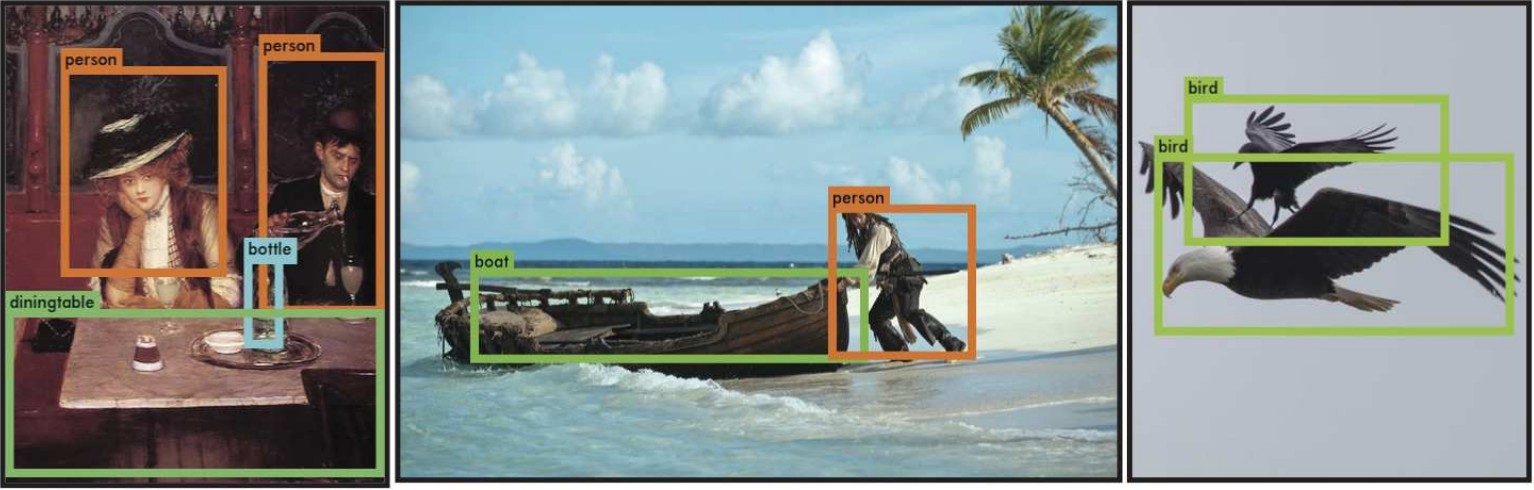
\includegraphics[width=15cm]{images/yolo.png}
	\caption{A YOLO osztályozó által megtalált befoglaló dobozok. \textit{Forrás:} \cite{redmon2016you}}
	\label{fig:yolo}
\end{figure}

A képek osztályozásához általánosságban \textit{konvolúciós} hálózatot szokás alkalmazni. A konvolúciós rétegeket tartalmazó modell ezen rétegek segítségével nyeri ki az osztályozási művelet elvégzéséhez szükséges képi-jellegzetességeket. A digitális képek $n \times m$-es mátrixokként vannak reprezentálva, a mátrix egyes pontjai pedig szürkeárnyalatos képek esetében a pixel intenzitásának értékei, színes képek esetén pedig az adott színkeverés alapján a színcsatornák értékei. A konvolúciós rétegek a kernelek és a filterek segítségével oly módon nyerik ki a bemeneti képek jellegzetességeit, hogy figyelembe veszik a pixelek szomszédságait, ezáltal a képeken található információt egy kisebb dimenziószámú leírásba transzformálja. A kisebb dimenzióban reprezentált adatokon az osztályozási feladat egyúttal könnyebben elvégezhető, másfelől a megfelelően összeállított jellegvektorok segítségével a képen található információ általánosabb formáját kapja meg az osztályozó, csökkentve annak a veszélyét, hogy a modell jellegtelen pixelekre tanulja be az egyes osztályokat.

Kiemelném az \textit{Inception modell}-t \cite{szegedy2015going}, amely a Google kutatói által kifejlesztett mély konvolúciós hálózat. Fő céljuk egy olyan modell megalkotása volt, amely az \textit{ImageNet} adathalmaz \cite{deng2009imagenet} 1000 darab osztályára megoldja az osztályozási feladatot. Az eredeti modell 2014-es megjelenése óta három további verziót is megélt (v2/v3 \cite{szegedy2016rethinking}, v4 \cite{szegedy2017inception}). A modell az inverz probléma egyes megoldásai során is szerepet kap, így a dolgozat során a későbbiekben is említésre kerül.

Az irodalomkutatás során fellelt eredmények közül a legfigyelemreméltóbb eredmény a CLIP \textit{zero-shot} osztályozó \cite{radford2021learning}, amelyet az internetről összegyűjtött képeken és a hozzájuk tartozó szöveges leírásokon tanítottak be. A CLIP modell képes rövid leírásokat adni a kép tartalmáról és az egyes mondatokat valószínűségi értékekkel látja el. Vagyis a különféle annotációk helyett természetes-nyelvi leírásokat ad kimenetként egy-egy képhez. A modell az inverz problémakör egyes megvalósításában is feltűnik majd, amelyeket a következő alfejezetben ismertetek.

%TODO: Eredmények szemléltetésére clip ábra


\Section{Az objektumfelismerés inverz problémája}

Az objektumfelismerés inverz problémája alatt azt a feladatot értjük, amely során csupán a képekre vonatkozó információk állnak rendelkezésünkre és ezen adatok alapján a gépi tanulásos modellnek a lehető legjobban kell reprezentációt találnia egy-egy kimeneti kép formájában.
Ehhez nem csupán a bemeneti, általában természetes nyelvi szöveget kell értelmeznie a modellnek, hanem a kimeneti képek előállításának módja is megoldandó feladat.
A jelenlegi eredmények alapján különféle megközelítéseket láthatunk a problémára, viszont ha csak az eredmények rendezetlen halmazára tekintünk, akkor az aktuális kutatási irányokat nehéz észrevenni. Az eredményeket többféle szempont szerint is csoportosíthatjuk az átláthatóság megkönnyítése érdekében. Mivel a megoldandó probléma alapvetően is két részre osztható: a bemeneti adatok feldolgozása és a kimeneti kép előállítása, így első körben a csoportosítást ezen két tengely mentén külön-külön is elvégezhetjük.

Ha a kimeneti képek alapján szeretnénk csoportosítani a jelenlegi eredményeket, akkor megállapíthatjuk, hogy a legtöbb szerző fotórealisztikus megjelenítésre törekedett. A képek előállítására általában \textit{generatív} modellt alkalmaztak, amely a gépi tanulásos megoldások azon halmaza, melynek feladata, hogy új adatokat állítsanak elő. Két generatív modell alkalmazása figyelhető meg a jelenlegi kutatási irányokban, azok közül is a második közkedveltebb, a talált publikációk alapján.
A képek kigenerálásához vagy \textit{Variational Autoencoder} (VAE) architektúrán alapuló modellt alkottak meg \cite{ramesh2021zero}, vagy \textit{Generative Adverserial Network} (GAN) alapú megoldásokat \cite{dong2021unsupervised, reed2016learning, xu2018attngan, zhang2017stackgan} alkalmaztak.
Egy olyan publikációt is találtam, amely figyelemreméltó módon nem generatív modellt alkalmazotta képek szintetizálására, hanem teljesen egyedi megközelítést, amelyben csupán Bézier-görbék halmazán végezték el az optimalizálást és eredményül rajzokhoz hasonló képeket kaptak. A módszert CLIPDraw-nak nevezték el \cite{frans2021clipdraw}, amelynek a nevében megtalálható, a már korábban említett CLIP osztályozó is.

A GAN és VAE részletesebb összehasonlítására egy későbbi fejezetben kerül sor. A saját módszeremhez szükséges képek előállítására szolgáló komponens alapjául, a különféle eredmények és a két módszer előnyeinek és hátrányainak figyelembe vételével úgy döntöttem, hogy egy GAN-t választom.
A GAN-hoz is igen szerteágazó kutatási irányok alakultak ki az évek során, amelyekben a közös cél természetesen az eredeti GAN kiegészítése oly módon, hogy a betanított modell a lehető legjobb eredményeket nyújtsa.

%TODO GAN hivatkozási gráf beillesztése, kis magyarázat írása az egyes irányokról és hogy mi az, amit átvettem belőlük...

\begin{figure}[h]
	\centering
	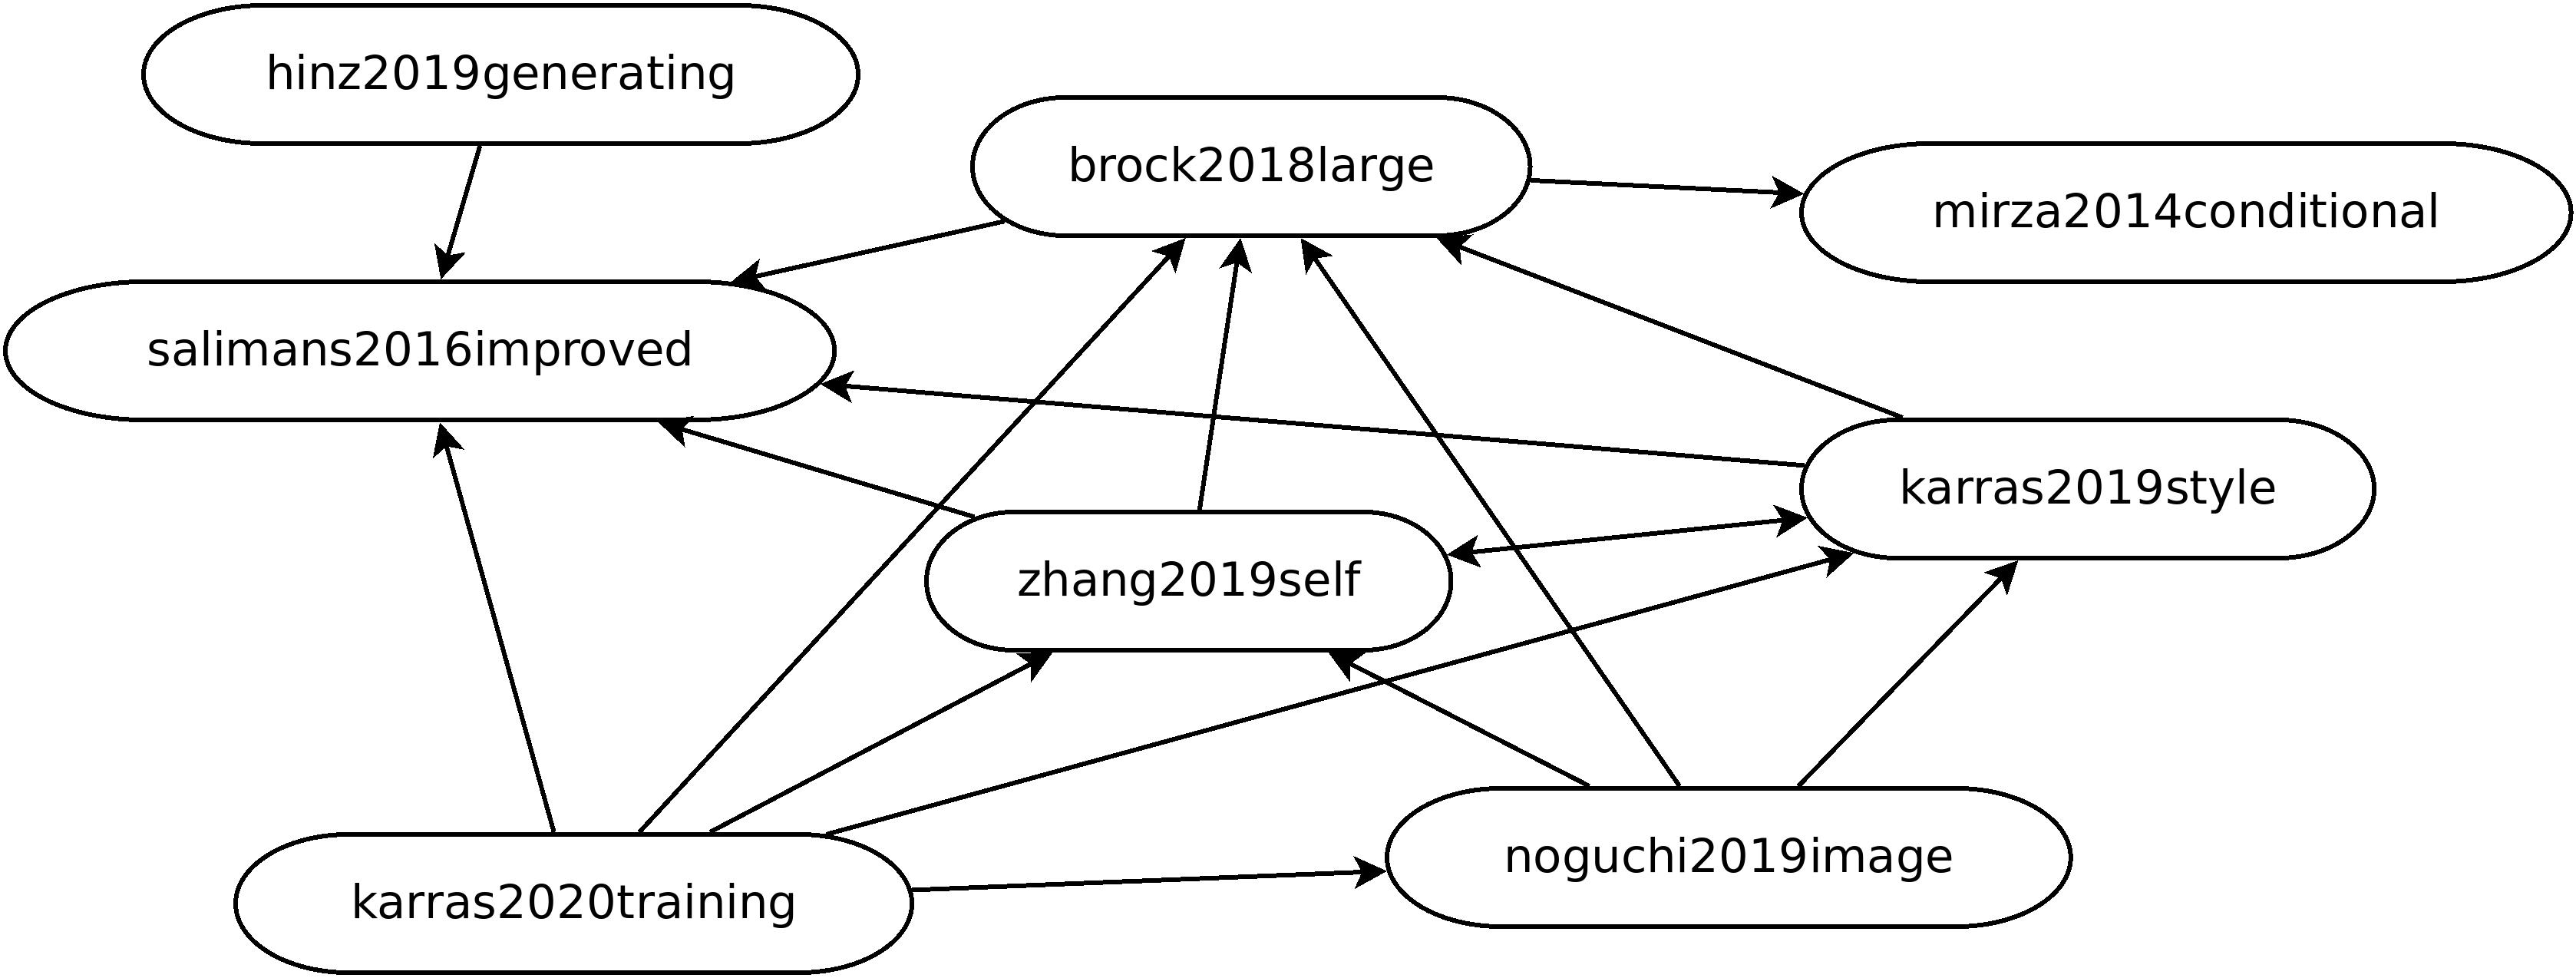
\includegraphics[width=15cm]{images/gancite.png}
	\caption{Hivatkozási gráf}
	\label{fig:gancite}
\end{figure}

% TODO: Problémakör bemutatása, különböző szerzők eredményeinek ismertetése, a képek generálásán kívül - szöveg feldolgozás és optimalizálás

\Section{Saját architektúra}

A kutatásom során szerzett ismeretek alapján a \ref{fig:architecture} ábrán szemléltetett architektúrát alkottam meg.

\begin{figure}[h]
\centering
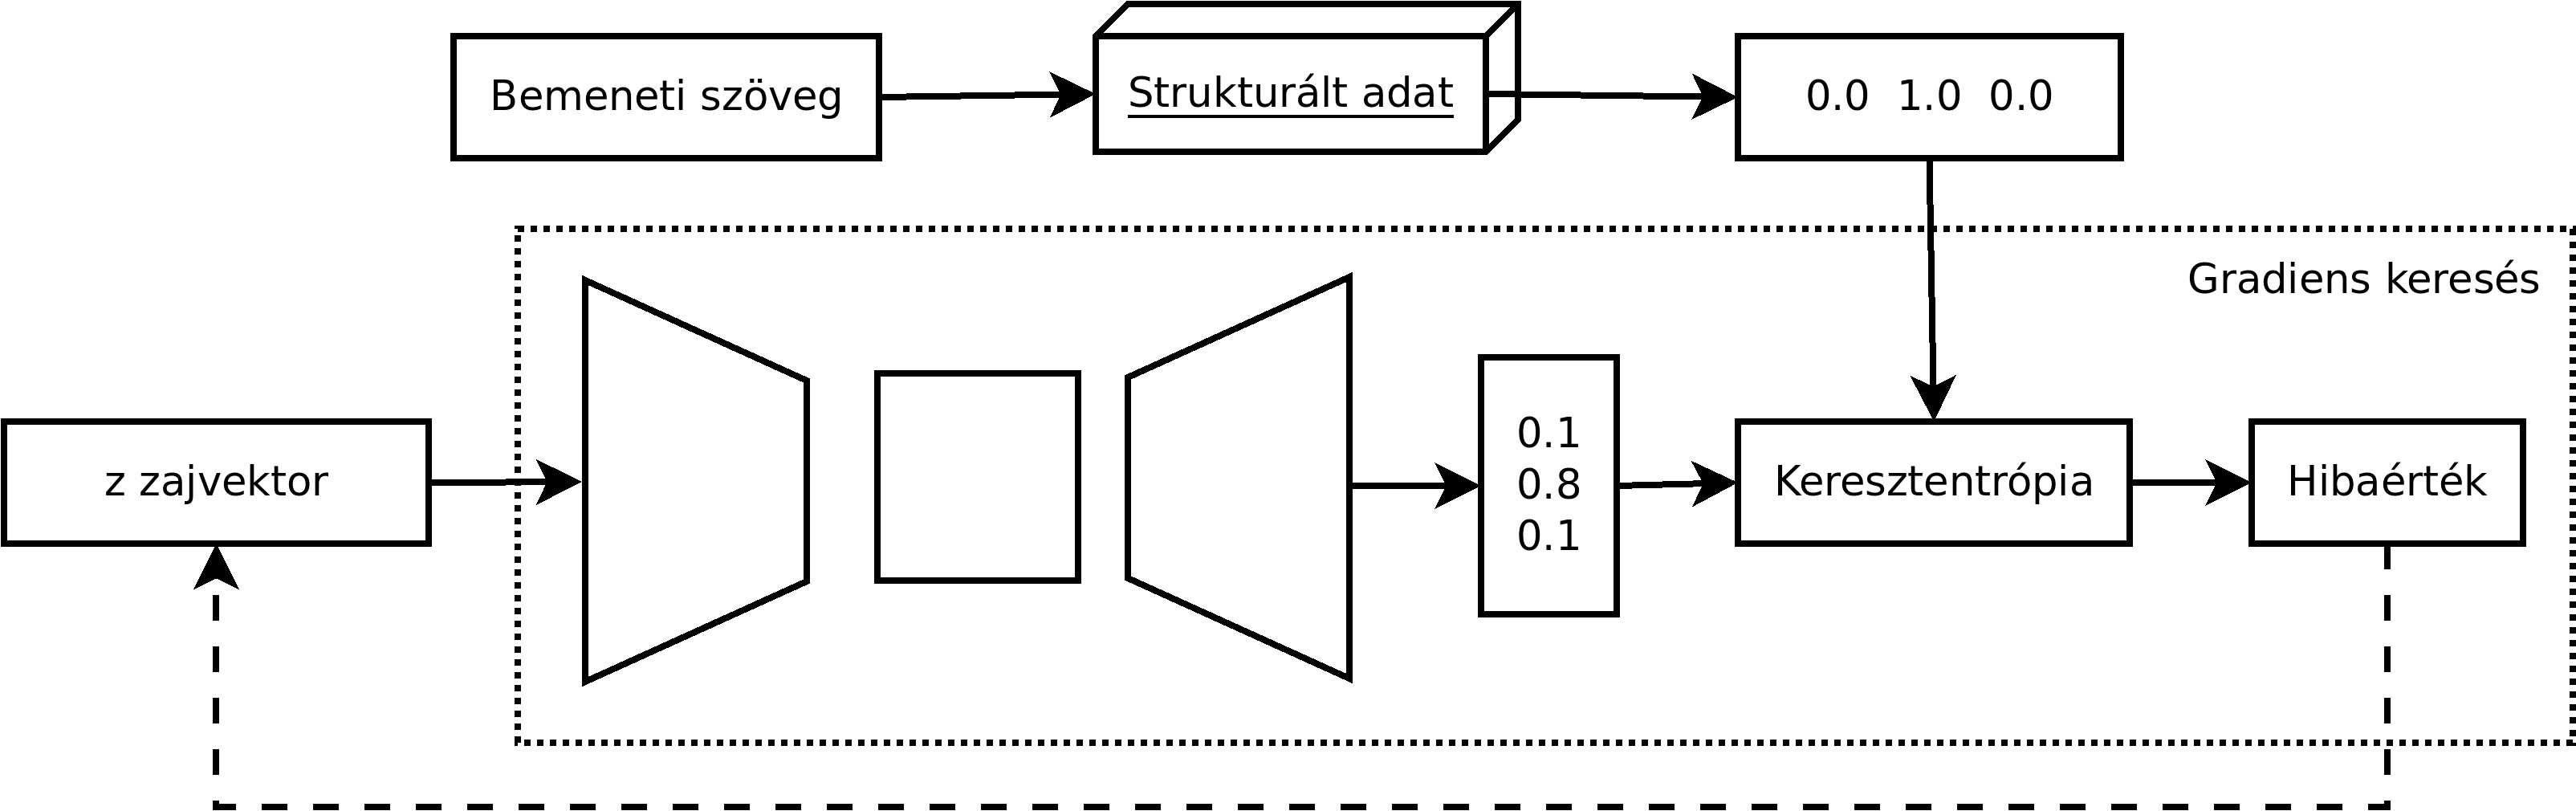
\includegraphics[width=15cm]{images/architecture.png}
\caption{Architektúra}
\label{fig:architecture}
\end{figure}

Az architektúra részei:

\begin{itemize}
	\item Bemeneti szöveg feldolgozó
	\item Strukturált adat enkódoló
	\item Optimalizáló modul
		\begin{itemize}
			\item Optimalizálandó zajvektor
			\item Képeket előállító háló (G)
			\item Osztályozó (D)
			\item Hibafüggvény számoló
		\end{itemize}
\end{itemize}

Az architektúra egy olyan zajvektort keres, amely a képeket kigeneráló háló bemeneteként a megfelelő képet előállítja.
A megoldásom egyes részei különféle megközelítési módszereken keresztül kerülnek ismertetésre a dolgozat további fejezeteiben.

%TODO: Mihez hasonlít ez? Miből mit vettem át?

\Section{Tensorflow és Keras}

A dolgozat programjának megvalósításához a TensorFlow függvénykönyvtárat választottam ki. A TensorFlow egy ingyenes, open-source gépi tanulásra használatos függvénykönyvtár, amely elsősorban mély- és gépi-tanulásos alkalmazások implementálására használatos. Számos programozási nyelvhez érhető el az API-ja, beleértve a Python, Java, C++ és JavaScript nyelveket. Viszont az API fő fejlesztési iránya a Python nyelvre összpontosul. A könyvtár a Google Brain fejlesztésében született meg 2015-ben, majd 2019-ben megjelent a 2.0-ás API verzió is, amely az API váltásból adódóan visszafelé nem teljesen kompatibilis az elsővel. Jelenleg a 2.8-as számozású stabil kiadással rendelkezik, a dokumentációja a \cite{tensorflow} forrás alatt érhető el. Az API lehetőséget ad az elosztott tanításra is. A betanított modellek széles körben alkalmazhatóak, akár web- vagy mobilalkalmazásokba is integrálhatóak. 

A Keras függvénykönyvtár egy interfészt biztosít a TensorFlowhoz. Segítségével igazán egyszerűen, modulárisan és átláthatóan állíthatunk össze neurális hálózatokat. Az általa biztosított eszközkészlet igazán változatos. A modellek összeállítására is többféle lehetőségünk van, például a \textit{Sequential API} használatával pipeline szerű modelleket építhetünk a különféle rétegek egymás után illesztésével. A \textit{Functional API} segítségével pedig igazán komplex kapcsolatokkal rendelkező architektúrák is megvalósíthatóak, a kódbonyolultság növekedése nélkül. A Keras korábban több backend-et is támogatott, viszont a legfrissebb verzióiban csak a TensorFlow-hoz alkalmazható. Látható, hogy a két könyvtár mennyire összefonódott. A dokumentációja a \cite{keras} forrás alatt érhető el.

Python-ban a \texttt{tensorflow} csomag az alábbi kódrészlettel importálható. A TensorFlow tartalmazza a Keras-t is modul formájában. Amennyiben nem importáljuk be külön a modult, úgy a \texttt{tf.keras}-al is elérhetjük, viszont az alábbi kódrészletben a Keras is importálásra kerül. A dolgozatban található kódrészleteknél az alábbi két sort nem tüntetem fel a továbbiakban, egységesen minden kódrészlethez az alábbiak szükségesek, a kivételt képző eseteknél, ahol szükséges lehet további csomagok importálása is, külön ki fogom emelni. (nem biztos, hogy lesz ilyen...)
\begin{python}
import tensorflow as tf
from tensorflow import keras
\end{python}

A dolgozathoz elkészült programokat \textit{IPython Jupyter notebook}-ok \cite{jupyter} formájában kerültek megvalósításra.

\Section{Modellek tanítása}

A mély neurális hálózatok tanítása igazán erőforrás-igényes feladat. A tanítható hiperparaméterek paraméterek nem ritkán milliós nagyságrendűek, a dataset-eknek pedig kellően nagynak kell lenniük, a feldolgozandó adatoknak pedig memóriába is bele kell férnie. Egy-egy iteráció igen sok időbe telhet egy gyengébb hardveren.

A kezdeti demóprogramok futtatása során szembesültem a első nehézséggel: A laptopom nem volt a legalkalmasabb nagyobb gépi-tanulásos modellek tanítására, hiszen igen sok időt vett igénybe a legkisebb példák futtatása is. Megoldásként egy olyan szolgáltatást kerestem az interneten, amellyel a dolgozatom programjához történő modelleket kényelmesen be tudnám tanítani.

A TensorFlow honlapján felleltem a Google Colab \cite{colab} felületet, amely ingyenes virtuális környezetet biztosít az IPython notebook-ok szerkesztéséhez és futtatásához. A felület egy előre meghatározatlan ideig GPU-t (Tesla K80) és TPU-t is biztosít kipróbálás jelleggel. Az ingyenes verzióban a napi GPU használatának limitje nincsen meghatározva, így egy idő után lekapcsolhatják és GPU nélkül megnövekszik a tanítás hossza. Továbbá a környezetet 12 óránként újraindítják, így minden adat elvezhet és csak akkor futhat a script, ha meg van nyitva a böngészőablak. Így az ingyenes verzió kisebb példák futtatására elegendő csupán és egészen korlátozott az ingyenes verzió használata. Természetesen a Tensorflow és a Keras ajánl lehetőségeket a modellek mentésére vagy a tanítás közbeni checkpoint-ok készítésére.

Például az alábbi kódrészlet futtatásával tetszőleges attribútumokkal létrehozhatunk egy checkpoint objektumot, amely segítségével mentéseket csinálhatunk a checkpoint paramétereiként megadott objektumok állapotairól. Ha esetleg a kimentett állapotokat vissza kívánjuk állítani, úgy a \texttt{checkpoint.restore()}-al a megfelelő fájlnév megadásával megtehetjük.
\begin{python}
checkpoint = tf.train.Checkpoint(
    generator_optimizer=generator_optimizer,
    discriminator_optimizer=discriminator_optimizer,
    generator=generator,
    discriminator=discriminator
)
checkpoint.save(file_prefix)

checkpoint.restore(checkpoint_path)
\end{python}

Egy másik lehetőségként lementhetjük a teljes modellt, amelyet később egyszerűen be is tölthetünk.
\begin{python}
model.save("./my_model")

new_model = keras.models.load_model("./my_model")
\end{python}
Ennek a módszernek az előnye, hogy nem szükséges a modell-t üresen deklarálni a betöltéshez, viszont a checkpoint-tal ellentétben a verziók nincsenek automatikusan menedzselve és erről nekünk kell gondoskodni. Az ilyen mentést a már betanított modellekhez javasolt megtenni, míg a checkpoint a tanítás során nyújt lehetőséget a biztonsági mentések készítésére. A saját modelleim tanítása során is felléptek olyan állapotok, amikor a modell használhatatlanná vált. Ilyen esetekben a biztonsági mentésekkel igen könnyedén vissza lehetett állítani az utolsó stabil állapotot.

Viszont számomra a Google Colab ingyenes próbaverziója nem volt teljesen megfelelő, a kiszámíthatatlanság miatt. Az előfizetés még csupán néhány kijelölt országban elérető, így Magyarországon jelenleg nem lehet a fizetős szolgáltatásra feliratkozni, így újabb felületet kellett keresnem.
Egy fórumon böngészve találtam rá a Kaggle \cite{kaggle} felületre, amely hasonló környezetet kínál, mint a Colab. Az alap. A Kaggle által biztosított virtuális környezet hardvere jobbnak bizonyult a Colab-bbal szemben. A GPU használat heti szinten kerül meghatározásra órákban, ami csak a használat során számolódik. Továbbá lehetőséget kínál a notebookok ütemezett futtatására is és az Kaggle-ön megtalálható bármelyik datasetet könnyedén betölthetjük és használhatjuk. Mindezen előnyök miatt a Kaggle-t választottam a modelljeim tanítására.

Az alábbi táblázatban található meg a laptopom és a Kaggle által biztosított környezet specifikációi:
\begin{center}
\begin{tabular}{ p{1.2cm}||p{6cm}|p{6cm}  }
	  & Dell Insprion-5558 & Kaggle környezet\\
	\hline
	\textbf{CPU} & 4x Intel(R) Core(TM) i3-5005U CPU @ 2.00GHz & 2x Intel(R) Xeon(R) CPU @ 2.00GHz\\
	\textbf{RAM} & 2x 4GB DDR3 1600 MHz & 15GB\\
	\textbf{GPU} & Intel HD Graphics 5500 (VGA) & Nvidia Tesla P100-PCIE-16GB\\
	\textbf{HDD} & 1TB & 73GB
\end{tabular}
\end{center}
A három környezet (laptop, Colab, Kaggle) teljesítményét egy általam felállított méréssel vizsgáltam.
A \texttt{RuntimeMeasure.ipynb} notebook használatos a mérés elvégzéséhez.
A teljesítménymérés alapja egy olyan GAN hálózat, amelyet meghatározott paraméterekkel hozunk létre.
A tanítás során az alábbi paraméterek változatlanok:
\begin{center}
\begin{tabular}{ c|c|c|c }
	Látens dimenziószám & mini-batch méret & filterek száma & kernelméret\\
	\hline
	100 & 32 & 128 & ($3\times 3$)
\end{tabular}
\end{center}
A felbontásnövelő rétegek száma a futó paraméter, amelyet 0-tól 3-ig vizsgálunk.
A hálózat felépítése megegyezik a DCGAN architektúrával, azzal az eltéréssel, hogy a Generátor utolsó dekonvolúciós rétege helyett egy konvolúciós réteg található, amely csupán dimenziócsökkentési feladatot végez, vagyis a feature-öket a három színcsatornába transzformálja. Hasonlóan a Diszkriminátorban is, az első konvolúciós réteg a bemeneti kép csatornáit bővíti ki, nem végez kicsinyítést.
A hálózatot 5 epoch-ig tanítjuk az adott felbontásnövelő rétegek mellett, majd az átlagos futásidő kerül lejegyzésre.
A mérés során a hálózatot a Cifar10 \cite{krizhevsky2009learning} adathalmazon tanítottam, labelek nélkül a train részhalmazán.
A mérés egyes állomásain a generátor különféle felbontásokban generálja a képeket. Így a tanítás előtt a tanítóhalmaz képeit is a generátor kimenetével megegyező méretekre kell skáláznunk.

A generátor kimenete a felbontásnövelő rétegek számával változik. Ha nem alkalmazunk ilyen réteget, akkor az ($4 \times 4$) felbontású képeket eredményez, majd rendre 1 réteg esetén ($8 \times 8$), 2 rétegnél ($16 \times 16$) és 3 rétegnél pedig ($32 \times 32$) felbontású képek jelennek meg a generátor kimenetén. A diszkriminátort is ennek megfelelően át kell alakítanunk, ott viszont a felbontáscsökkentő rétegek számát kell módosítanunk. Mivel a felvázolt GAN szimmetrikus, így a felbontásnövelő és felbontáscsökkentő rétegek száma megegyezik.

\begin{python}
...
for i in range(upsampling_layers):
    hidden = keras.layers.Conv2DTranspose(
        units_per_layer, kernel_size, 2, 'same'
    )(hidden)
    hidden = keras.layers.BatchNormalization()(hidden)
    hidden = keras.layers.ReLU()(hidden)
...
\end{python}

A generátorban és a diszkriminátorban is egy-egy for ciklussal megoldhatjuk az említett rétegek hozzáadását a hálók építésénél. A fenti példa kód szemlélteti a generátorban lévő dekonvolúciós réteg hozzáadását.
A notebookot futtatva a különböző környezeteken a \ref{fig:runtime} ábrán látható eredmények jöttek ki.

\begin{figure}[h]
\centering
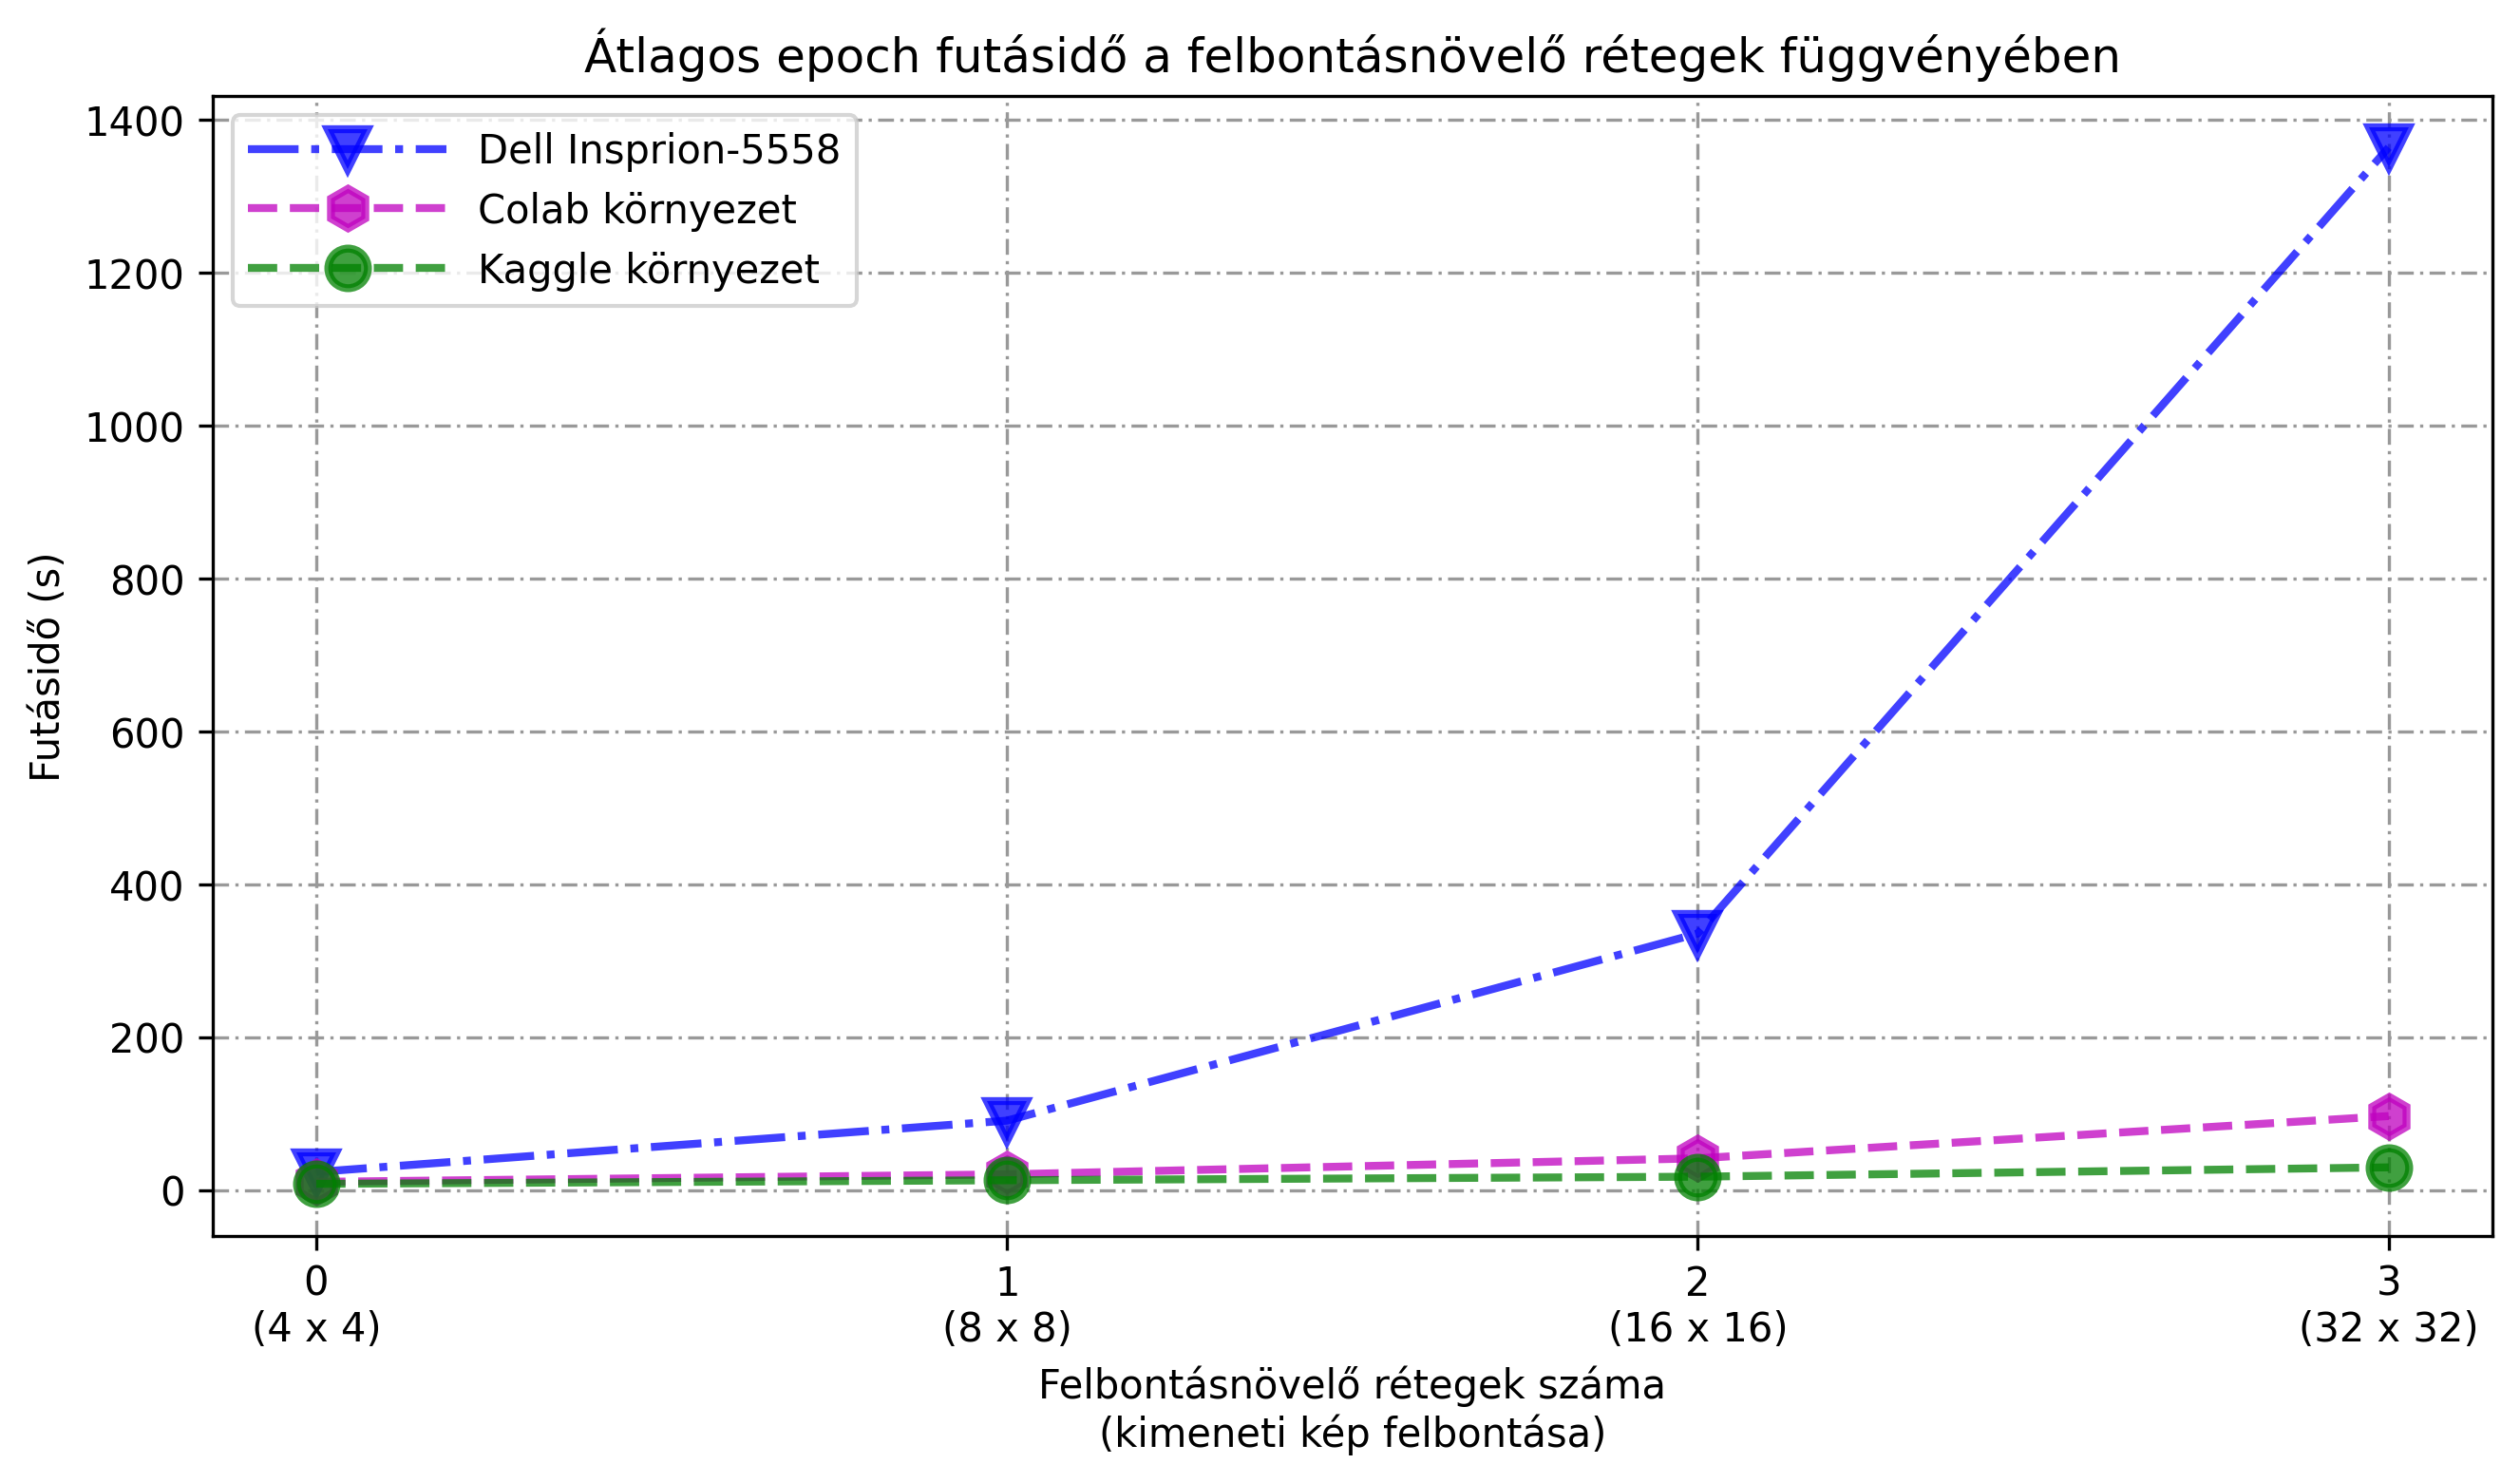
\includegraphics[width=15cm]{images/runtime.png}
\caption{Runtime ábra}
\label{fig:runtime}
\end{figure}

Mint látható, a laptopom igen alulmaradt a két virtuális környezettel szemben és érzékelteti az ábra, hogy saját munkaálláson mennyire megnehezedik a tanítás a várakozási idők meghosszabbodásával. A modellek összeállításának kezdeti fázisaiban több prototípus készült el, mire eljutottam a végleges változatig. Az egyes próbálkozások a megfelelő modell kiválasztására a laptopomon nagyon sok időt vett volna el, amely rontotta volna a kutatás hatásfokát is.

\newpage

\Section{A tanításhoz használt adathalmazok}

A tanításhoz szükségünk van egy megfelelő adathalmazra. Képek generálásához legegyszerűbb esetben elegendő lehet képek rendezetlen halmaza is és a modellre bízhatjuk, hogy ismerje fel az egyes osztályok jellegzetességeit. Megfelelő regularizációs technikákkal igazán változatos képek generálására lesz képes a betanított modell.

Ha az adathalmaz rendelkezik osztályokkal is, úgy az osztály-címkéket is felhasználhatjuk a GAN hálózatunk tanításához. Így egy plusz bemenet segítségével könnyebben tudunk majd megfelelő képeket előállítani. (Ezt a technikát class-conditioning-nak nevezik, de utána kell nézzek)

Egyes adathalmazokhoz igen részletes annotációkat is mellékelnek. A képeken megfigyelhető objektumokat határoló dobozokkal, vagy pixel szinten is jelölik. Így igen részletes információkat kínálnak a kép tartalmáról. Egy igazán hasznos annotációk lehetnek a természetes nyelvű leíró mondatok is, amelyekből általában többet is mellékelnek egy-egy képhez.

Ha kiválasztottuk a modellünkhöz megfelelő adathalmazt, akkor a probléma és a modell bonyolultságától függően elő kell készítenünk az adatokat a tanításhoz.

Az irodalomkutatás során talált egyes GAN modellek esetén megfigyelhető, hogy a fotórealisztikus eredmény érdekében a tanításhoz használt adathalmazt erősen tisztították és általában egyetlen egy doménból származnak az adatok. Tehát pédául a CelebFaces vagy az Oxford Flowers vagy a CUB esetében.

%TODO: Példák az adathalmaz elemeire, pontosítás

\begin{itemize}
	\item Animal Faces-HQ (AFHQ) \cite{choi2020stargan}\\
		Az adathalmaz állatokról tartalmaz portrékat igen jó minőségben. A színes fényképek felbontása $ 512 \times 512 $, az állatok fotói pedig pozicionálva vannak a szemük szerint. Tehát igen tisztának lehet nevezni az adathalmazt. A dataset-et bevezető publikációban azt is megemlítik, hogy kézi szelektálást is végeztek, hogy a lehető legjobb minőségű legyenek a minták. A mintákat 3 osztályban adták meg: Kutya, macska és vadállat. Az osztályokban egyenként 5000 tanítóminta található, így összesen 15 ezer képből áll az adathalmaz. A kevés osztály ellenére az osztályokon belül igen változatos képek figyelhetők meg, a fajok különböző alfajaira.
	\item Cifar-10 \cite{krizhevsky2009learning}
		A Cifar-10 adathalmaz valójában a Cifar-100 adathalmaznak egy leszűkített változata. Az utóbbi 100 osztályt magába foglaló adathalmaz, míg a Cifar-10 csupán 10 class-al rendelkezik. A tanítóhalmaza 50000 képet tartalmaz.
		Az adathalmaz képei ($32 \times 32$) felbontásúak és 3 színcsatornával rendelkeznek (RGB).
\end{itemize}

\Chapter{Bemenet feldolgozása}

Az inverz probléma bemeneteként az eredeti, objektumfelismerési probléma kimeneteire lesz szükségünk. A Koncepció fejezeteben az objektumfelismerés áttekintésében említésre kerültek a lehetséges kimenetek. Ha osztályozási feladatot értünk az objektumfelismerés alatt, akkor a felismerő modell kimenetén az egyes osztályok valószínűségi értékei figyelhetők meg. Az általam elkészített implementáció is valójában ilyen adatokat vár, majd ezen adatok szerint hajtja végre a képek kigenerálását.

Ezen fejezet a \ref{fig:architecture} ábrán megfigyelhető \texttt{Bemeneti szöveg} és a \texttt{Strukturált adat} részeivel foglalkozik. Vagyis a bemeneti adatok feldolgozásával, amelyek a további komponensek működéséhez szükségesek.

Az osztályokra vonatkozó adatokat a modell természetes nyelvű szöveg formájában kapja meg. A bemeneti szöveg ezután az általam megadott szabályok szerint strukturált adattá alakul, amelyben a különféle osztályok súlyozásai szerepelnek.

A képek generálást elvégző modelljeim olyan adathalmazokra tanultak, amelyekben meghatározott számú osztály található. Viszont például a Cifar-10 esetén az osztályok csupán egész számokkal vannak jelölve 0-10-ig és így minden esetben ki kell keresni, hogy melyik szám mit jelent. Tehát ehhez az adathalmazhoz nincsen konkrét szöveges adat, csak a publikált táblázatból olvashatók ki a az osztályokhoz tartozó címkék. Egy olyan megoldást kívánok bemutatni, amely nem szorul gépi tanulásos módszerekre és egyszerű szinonima szótár segítségével detektálja a mondatokban szereplő objektumokat.

\Section{Természetes nyelvi szöveg feldolgozása}

A bemeneti szöveget magyar nyelven várja a program. A szövegnek egy olyan leíró mondatnak kell lennie, amely a kigenerálandó kép tartalmát írja le, vagyis, hogy mi szerepel a képen. Mivel a képek generálásáért felelős komponensem csupán osztályokat tud kigenerálni, így a képen egy-egy objektum figyelhető meg csupán. Eszerint csak olyan bemeneti mondatokat tud értelmezni a program, amely az általa ismert osztályokra vonatkozik. Viszont lehetőség van kevert osztályok megadására is, különféle súlyokkal, amit kétféleképpen lehet megadni. Ha a bemeneti mondatot olyan kifejezésekkel látjuk el, amelyben több osztály is megfigyelhető, úgy a mondat feldolgozása után kapott strukturált adatban az említett osztályok hasonló súlyozással fognak szerepelni. Egy másik lehetőségként százalékos értékekkel is elláthatjuk a kigenerálandó objektumokat. A kigenerált képen továbbra is egy objektum figyelhető majd meg, viszont olyan kép kerül előállításra, amely az említett osztályok tulajdonságait hordozza a megadott súlyozás szerint.

Valójában a bemenet ilyen formában várása csupán egy felhasználó élményt növelő funkció. Az interakció ilyen formája minden bizonnyal természetesebbnek hathat a felhasználói oldalon. Ha egy olyan képgeneráló modellel kívánunk dolgozni, amely több osztályt ismer, akkor a bemenet ilyen formában történő bevitele tűnhet a legegyszerűbbnek a felhasználó számára.

A bemeneti mondat egy egyszerű normalizálási folyamaton megy keresztül, hogy a további feldolgozást megkönnyítse. A normalizálási folyamat a következő:

\begin{enumerate}
	\item Írásjelek eltávolítása
	\item A szöveg kisbetűssé tétele
	\item A szavak kigyűjtése (tokenek megalkotása)
	\item A százalékos értékeket jelző tokenek szerializálása
\end{enumerate}

Az utolsó pont csupán egy olyan műveletet jelöl, amely során a százalékos értékeket képviselő tokeneket egy egységesített formában hozza, hogy a következő lépésben könnyebben lehessen kezelni ezen értékeket. Ha a tokenizálás során az érték és a százalék szimbólum két külön tokenbe került, akkor ilyen esetben a két token egységesítődik és egy tokenként él tovább. Ha esetleg a bemenetben az érték után a "százalék" szóval került megadásra a $\%$ szimbólum, úgy a "százalék" szó törlésre kerül és egységesen a $\%$ szimbólum kerül az értékek mögé.

Ezen szabályok természetesen elég egyszerűek és specifikusak és csupán a már említett strukturált adatok megalkotásához szükségesek a bemeneti mondatok.

További normalizáló lépés is létezhet. Például a szavak toldalékainak leválasztása (\textit{stemming}) vagy a jelentéshez nem feltétlenül szükséges kötőszavak kiszűrése is használható a normalizálásban \cite{bird2009natural}. Mivel a bemeneti mondatok elég specifikusak és kicsit kötöttek is, így további normalizálás nem lett alkalmazva a bemenetre a felsoroltakon kívül.

\Section{Strukturált adatok megalkotása}

Ha a bemeneti mondat normalizálásra került, úgy előállítható belőle a strukturált adat, amely jelen esetben \textit{python dictionary} formátumban kerül megalkotásra. A strukturált adatok kinyerése a szövegből egyik technikája a \textit{Named Entity Recognition} \cite{bird2009natural}, amely az egyes tokeneket osztályozza a szövegben elfoglalt helyük és szófajok figyelembevételével. A dolgozatom ezen része nem terjed ki olyan részletesen a Természetes Nyelvi Szövegfeldolgozásra, a rendelkezésre álló adatok hiányában egy egyszerűbb megoldást választottam, amely szinonima szótár segítségével osztályozza a megfelelő tokeneket.

Az egyes modellekhez használatos szinonima szótár megalkotásához segítségemre volt az interneten talált szinonimaszotar.hu honlap \footnote{Magyar internetes szinonimaszótár \url{https://szinonimaszotar.hu}.}. Ezen példákhoz elegendőnek éreztem a szinonimák használatát is, viszont több osztályt ismerő modellek esetén a megoldásom valószínűleg már kevésbé lesz pontos, hiszen csupán a nyers szavakat hasonlítja össze betű szinten. Egy kifinomultabb megközelítés a szófajok, ragozás és mondatszerkezetek vizsgálata lehet. Vagy egy olyan \textit{embedding} megalkotása, amely az egymáshoz hasonló jelentésű szavakat közelebb helyezi el a belső terében, mint például a \textit{Word2Vec} \cite{mikolov2013efficient} módszer esetében, amely jelenleg csupán csak behivatkozásra kerül, ugyanis nem tettem ilyen jellegű vizsgálatot a dolgozatom során.

A mondat szavain egyesével megy végig az algoritmus, és összehasonlításra kerülnek a szavak az elkészített szinonimaszótár elemeivel. Amennyiben egy szinonima megtalálható a vizsgált szóban egy bizonyos mennyiségben, úgy a szót a szinonimához tartozó osztállyal látjuk el. A tartalmazás vizsgálata százalékos módon kerül kiértékelésre és a vizsgált szinonima pedig a szóban bárhol elhelyezkedhet, a betűk egyezése számít csupán. A 80\%-os egyezés vizsgálata megfelelőnek tűnt a példák futtatása során. Az összetett szavak vagy a prefixekkel, esetleg a ragokkal ellátott szavak alapjaiban az eredeti szó megfigyelhető, így elegendőnek éreztem ilyen szintű egyezés vizsgálatát is. Természetesen a jelentésbeli vizsgálat nem történt, így például a "ló" szó a "halló" szóban 100\%-os tartalmazást fog mutatni, annak ellenére, hogy egészen mást jelentenek a szavak.
Ezen módszer kevés osztályok mellett és megfelelő bemenetekre használható eredményeket szolgáltat, viszont a saját tudásbázisán kívül már nem képes megfelelően eredményeket adni.

A százalékos értékek az előző feldolgozási lépések alapján kerülnek detektálásra és feldolgozásra. Amennyiben az előző lépésben az osztályok megtalálásra kerültek és ha előttük található százalékos érték, akkor a strukturált adatban a megfelelő értékekkel kerülnek bejegyzésre. Ha nem minden detektált osztályhoz található százalékos érték, úgy a maradék értékek az említett osztályok között kiosztásra kerülnek.
Amennyiben megtalált valószínűségi értékek összege nem egyre jön ki, úgy a maradék osztályok között kerülnek szétosztásra az értékek. Ha a bemeneti mondatok nem tartalmaznak százalékos értékeket, úgy a mondatokban azonosított osztályok azonos súlyozással kerülnek rögzítésre.

A következő három példán megfigyelhető, hogy az egyes bemeneti mondatokra milyen strukturált adat készül el. Az első két példa az AFHQ-, míg az utolsó a CIFAR-10 osztályaira lett alkalmazva.

\noindent\textit{Egy vadkutya portréja található a képen.}
\small{
\begin{verbatim}
{
    'cat': 0.0,
    'dog': 0.5,
    'wild': 0.5
}
\end{verbatim}
}

\noindent\textit{75 \% macska van a képen, 25 százalék pedig öleb.}
\small{
\begin{verbatim}
{
    'cat': 0.75,
    'dog': 0.25,
    'wild': 0.0
}
\end{verbatim}
}

\noindent\textit{Fotó egy olyan lóról amely 30\%-ban agancsos.}
\small{
\begin{verbatim}
{
    'airplane': 0.0,
    'automobile': 0.0,
    'bird': 0.0,
    'cat': 0.0,
    'deer': 0.3,
    'dog': 0.0,
    'frog': 0.0,
    'horse': 0.7,
    'ship': 0.0,
    'truck': 0.0
}
\end{verbatim}
}

A példákban található egyéb kifejezéseket nem veszi figyelembe az algoritmus. Csupán az általa ismert osztályokra vonatkozó információk kerülnek kinyerésre, mivel a képet előállító komponens is csak ezen adatok alapján tud képet generálni. Egy fejlettebb modell esetében vizsgálatra kerülhetnének a számosságot, helyzetet jelölő szavak is például. Vagy az adott objektum egyes tulajdonságait leíró kifejezések, mint például a színre vagy textúrára vonatkozó megkötések is. Viszont a dolgozatban ezek sem kerültek vizsgálatra.

\Chapter{Új adatok előállítása, generatív modellek}
A generatív modellek alatt olyan gépi-tanulásos architektúrákat értünk, amelyek célja, hogy új adatokat állítsanak elő. A létrejött adatnak hasonlítania kell a tanítómintához, vagyis a generált minták eloszlásának közelítenie kell a valós adatok eloszlását. Az ilyen modelleknek meg kell tanulnia a tanítóminta jellegzetességeit és azt is, hogy ezen jellegeket a belső reprezentációjából hogyan tudná értelmezhető formában előállítani. A generatív modellek esetében ha a modell a tanítóminta képeit generálná csupán vissza pixel-pontosan, úgy a modell elveszti célját és egyfajta túltanulásnak (\textit{ovefitting}-nek) tekinthetnénk a jelenséget.

Az Autoencoder egy olyan statisztikai elveken alapuló architektúra, amelynek célja, hogy a tanítóhalmaz jellegzetességeit feltérképezze, és olyan formába kódolja a tulajdonságokat, hogy azokból az eredeti adat visszaállítható legyen. Az architektúra lényegében egy nehezen kezelhető sűrűségfüggvényt definiál, egy látens taggal, így ebben az esetben nem lehet közvetlenül optimalizálni, nem úgy mint például a pixelRNN/pixelCNN generatív modellek esetében \cite{oord2016conditional}, ahol az úgynevezett \textit{Evidence Lower Bound} (ELBO) mértékegységre kell optimalizálni\cite{oord2017neural}. Az architektúra két komponense az Encoder, amely előállítja a jellegvektorokat a bemenet alapján és a Decoder, amely a jellegvektorokból visszaállítja az adatot. Tehát ebben az esetben a cél az, hogy egy olyan reprezentációt készítsünk a tanítómintáról, amely alapján az teljes mértékben visszaállítható. Egyfajta tömörítési folyamatnak is felfogható az encoder működése. Egy módosított változattal az encoder által létrehozandó látens tér olyan formában áll elő, amelyből véletlenszerűen is vehetünk mintákat és dekódolva teljesen új adat áll elő. Ezt a módszert \textit{Vector Quantised-Variational AutoEncoder}-nek nevezték el, amely alkalmazható generatív modellként \cite{oord2017neural}.
Ha az autoencoder-t képek generálására kívánjuk felhasználni, úgy a helyreállított képeken egyfajta homályosságot figyelhetünk meg, amely a dekódolás során jelentkező információvesztésből adódik.

A \textit{Generative Adverserial Network} (GAN) \cite{goodfellow2014generative}, egy olyan generatív modell, amely nem a megszokott statisztikai alapokon optimalizál (mint például az Autoencoder vagy pixelRNN modellek), hanem játékelméleti megközelítést alkalmaz, így a modell tanítása is merőben másképp zajlik.
A tanulás során két neurális hálózat versenyzik egymással: egy generátor, amelynek az a szerepe, hogy a tanítómintákhoz hasonló adatot generáljon a bemeneti zajból és egy diszkriminátor, amely egy bináris osztályozó, amely a generátor által generált adatot vizsgálja és eldönti, hogy az valódi vagy hamis.
A tanítás során ezen két háló versenyzik egymással, együtt fejlődve. Az autoencoderhez képest a GAN-al generált képeken már nem figyelhető meg a homályosság, élesebb és fotórealisztikusabb képek generálására képes az eredmények alapján.

A generátor bemenete egy zajvektor, amelyet általában Gauss- vagy egyenletes eloszlásból állítunk elő. A zajnak a terét az irodalom látens térnek is nevezi, hiszen a tanítás során a modell megtanulja, hogy ezen többdimenziós tér egyes pontjaira milyen kimenetet generáljon. Vagyis ezzel lényegében kitölti a rendelkezésre álló tér tartományait a megtanult jellegzetességekkel. A betanított generátorral, optimális esetben, ezen tér bármely pontját mintavételezve a tanítóhalmazhoz hasonló adatokat generálhatunk.

\begin{figure}[h]
\centering
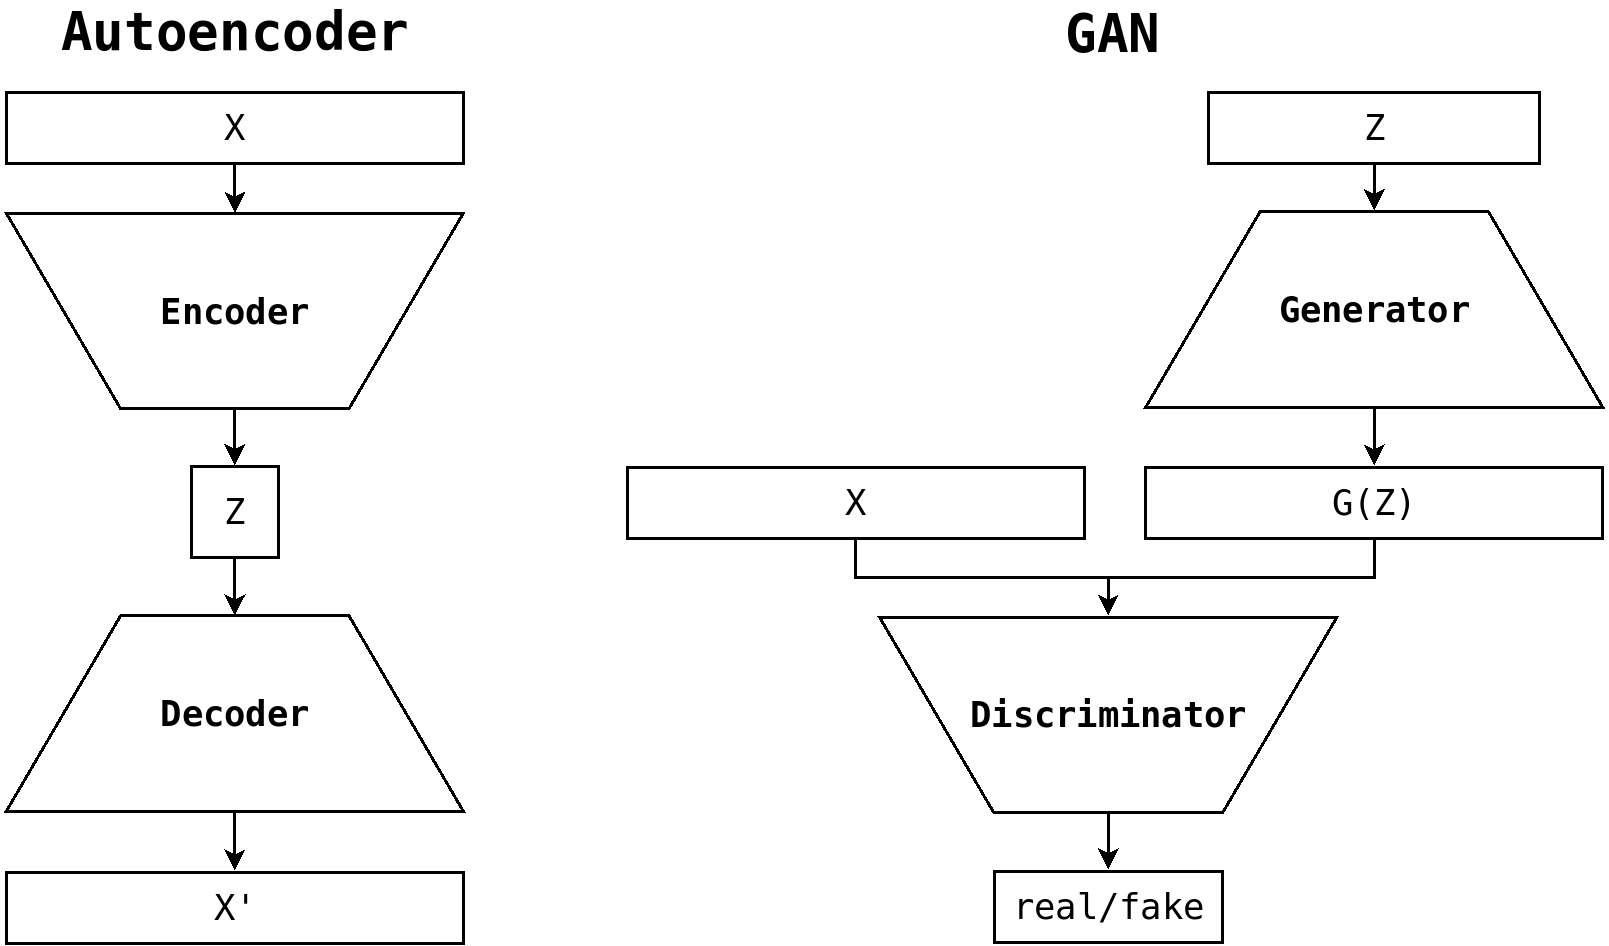
\includegraphics[width=12cm]{images/AEvsGAN.png}
\caption{Az Autoencoder és a GAN}
\label{fig:aevsgan}
\end{figure}

\Section{GAN modell tanítása}

A továbbiakban a következő jelöléseket használom: legyen $D$ a diszkriminátor, $G$ pedig a generátor.
Ha a legegyszerűbb esetet vizsgáljuk és csak a képek rendezetlen halmazára tanítjuk a modellt, mindenféle kiegészítő információ és annotáció nélkül, akkor a tanítás a következő pontokban leírtaknak megfelelően zajlik.

\SubSection{Hibafüggvények}

A $G$ és $D$ hibájának számolása a bináris kereszt-entrópián alapszik.
A bináris kereszt-entrópia hibafüggvény a következőképpen írható fel:
$$L(\hat y, y) = y \cdot \log \hat y + (1-y) \cdot \log (1 - \hat y),$$
ahol $\hat y$ a predikció, $y$ pedig a valós címke.

A Kerasban található implementáció egy segédfüggvényt ad vissza, amelyet különféle paraméterekkel inicializálhatunk.
\begin{python}
cross_entropy = keras.losses.BinaryCrossentropy(from_logits=True)
\end{python}
A \texttt{from\_logits=True} paraméter esetén a keresztentrópia számolásnál nem szükséges a diszkriminátor modellnek tartalmaznia az utolsó sigmoid aktivációs függvényét, ami így egy úgynevezett \textit{Logits} kimenettel fog rendelkezni. A számolás során a kimeneti értékekre alkalmazódik ebben az esetben a szigmoid függvény egy fajtája.

\SubSection{Diszkriminátor hibafüggvénye}

A $G$ generátor egy $z \in \mathbb{R}^n, n \geq 1$ bemeneti zajvektor alapján előállít egy generált adatot $G(z)$.
A $D$ diszkriminátor egy bináris osztályozó, amelynek feladata, hogy az $x$ és $G(z)$ bemeneteit osztályozza.
$D(x)$ esetén 1, $D(G(z))$ esetén pedig 0 címkét várunk.
A hibafüggvény számolása két lépésben történik a kétféle bemenet miatt.

$D(x)$-re nézve a kereszt-entrópia a következő:
$$L(D(x), 1) = 1 \cdot \ln D(x) + (1 - 1) \cdot \ln(1 - D(x)) = \ln D(x),$$
vagyis jelen esetben $D$-nek a $\ln(D(x))$-et kell maximalizálnia.

$D(G(z))$-re nézve a kereszt-entrópia a következő:
$$L(D(G(z)), 0) = 0 \cdot \ln D(G(z)) + (1 - 0) \cdot \ln(1 - D(G(z))) = \ln(1- D(G(z))),$$
vagyis a $\ln(1 - D(G(z)))$-t kell maximalizálnia.

Egyetlen mintára a hibafüggvény a következőképpen néz ki:
$$\max V(D) = \ln D(x) + \ln(1 - D(G(z)),$$
Batch-ra nézve:
$$\max V(D) = \mathbb{E}_{x \sim P(x)} \left[\ln D(x) \right] + \mathbb{E}_{z \sim P(z)} \left[\ln(1 - D(G(z))) \right],$$
ahol a $P(x)$ a valószínűségi eloszlása a tanítóhalmaznak, $P(z)$ a valószínűségi eloszlása a $z$ zajvektornak (látens térnek).

A hibafüggvény implementációja összességében az alábbi:
\begin{python}
def discriminator_loss(real_output, fake_output):
    real_loss = cross_entropy(tf.ones_like(real_output), real_output)
    fake_loss = cross_entropy(tf.zeros_like(fake_output), fake_output)
    
    total_loss = real_loss + fake_loss
    return total_loss
\end{python}

\SubSection{Generátor hibafüggvénye}

A $G$ generátor feladata az, hogy megtévessze a $D$ diszkriminátort azáltal, hogy a tanítóhalmazhoz hasonló adatokat generáljon.
Vagyis a $G$ érdeke az, hogy a $D(G(z))$ 1-es címkét kapjon 0 helyett.

A bináris keresztentrópia egy mintára:
$$L(D(G(z)), 0) = \ln(1 - D(G(z)).$$
$D$ minimalizálni kívánja a $D(G(z))$-t, míg a $G$ maximalizálni szándékozik azt.

A $G$ a tanítás során sosem fog valódi adatot látni, csupán a diszkriminátor hibáiból fog tanulni.

A generátorhoz tartozó hibafüggvény implementációja:
\begin{python}
def generator_loss(fake_output):
    return cross_entropy(tf.ones_like(fake_output), fake_output)
\end{python}

A GAN hálózat tanítása során $D$ és $G$ egy minimax játékot játszanak a $V(G, D)$ értékfüggvénnyel. Ez formálisan:
$$\min_{G}\max_{D}V(D, G) =  \mathbb{E}_{x \sim P(x)} \left[\ln D(x) \right] + \mathbb{E}_{z \sim P(z)} \left[\ln(1 - D(G(z))) \right].$$

\SubSection{Optimalizáló módszer}
A GAN modell súlyait a sztochasztikus gradiens algoritmussal szokás frissíteni.

A Generátort és a Diszkriminátort a hibafüggvények alapján kiszámolt gradiensek alapján külön-külön kell tanítani. Különféle szerzők különböző optimalizáló módszerek használatát javasolják, az Adam és az RMSProp a két legnépszerűbb módszer \cite{kingma2014adam}.

A saját implementációimban az Adam optimalizáló módszert alkalmaztam. A módszer legfontosabb paramétere a \textit{learning-rate}, vagyis a tanulási mérték. A 0.0001 learning-rate érték megfelelőnek tűnt a modelljeim tanítása során.

%TODO: Optimalizáló módszerek bemutatása akár egy ábrával vagy valami, hogy ez az alfejezet valahogy pontosabb legyen!

Az alábbi kódrészlet segítségével inicializálhatunk egy-egy példányt az Adam optimalizálóból a generátornak és a diszkriminátornak.

\begin{python}
generator_optimizer = keras.optimizers.Adam(1e-4)
discriminator_optimizer = keras.optimizers.Adam(1e-4)
\end{python}


\SubSection{Tanítási lépés}
A GAN esetében a hálózat paraméterei közé tartozik a mini-batch elemszáma is. Mini-batch alatt a tanítóhalmaz egy bizonyos elemszámú mintát tartalmazó szeletét értjük. A mini-batch-ek alkalmazása azért lényeges, hogy egy tanítási lépés során a modell ne lássa a teljes tanítóhalmazt. A hálózat tanításához általában sok mintára van szükségünk, így az egy darabban való tanítás igen nehézkes és számításigényes lenne. De nem csupán ez jelenti a fő veszélyt, Ha egy lépésben láthatná a diszkriminátor az összes képet, akkor túlságosan is megnőne a teljesítménye és a generátornak esélye sem lenne felzárkózni. A mini-batch-eken való tanítás tehát elengedhetetlen része a tanítási folyamatnak és a megfelelő ütemű tanulás biztosításának.
A fellelhető irodalomban a mini-batch-et néhány esetben röviden batch-nek nevezik. Viszont a batch egyes irodalmakban a teljes dataset-et jelöli, így az egyértelműség kedvéért minden esetben kiírom, hogy mini-batch.

%% GAN 2014 cikkből

Legyen $m$ a mini-batch elemszáma $m \in \mathbb{N}$
A GAN hálózat egy tanítási lépése a következő műveletekből áll \cite{goodfellow2014generative}:
\begin{enumerate}
\item Hozzunk létre $m$ darab zajmintát $(z_1, \ldots, z_m)$ normális eloszlásból $P_g(z)$.
\item A tanítóhalmazból emeljük ki a soron következő $m$ darab tanítómintát (képet), és ezt jelöljük $(x_1, \ldots, x_m)$-el. % $P_{\text{data}}(x)$
\item Frissítsük a $D$ diszkriminátort a sztochasztikus gradiens emelkedésével, amelynek értéke
$$ \nabla \theta_d \frac{1}{m} \sum_{i=1}^{m} \left[\log D(x_i) + \log(1 - D(G(z_i))) \right].$$
\item  Frissítsük a $G$ generátort a sztochasztikus gradiens süllyesztéssel:
$$ \nabla \theta_d \frac{1}{m} \sum_{i=1}^{m} \log(1 - D(G(z_i))).$$
\end{enumerate}

A GAN részeit tehát külön-külön tanítjuk, hiszen különböző neurális hálókról van szó. Az eredeti cikkben is javaslatot tesznek arra, hogy a $D$-t esetleg több lépésben is lehetne tanítani, majd a $G$-t egyetlen lépésben frissíteni.
Különböző tanítási stratégiákban ez is egy szabad paraméter lehet. Számomra megfelelő volt az 1:1-es tanítási lépés alkalmazása is. Viszont több cikkben is vizsgálják ezt, mint lehetséges beállítást.
A tanítás hossza természetesen függ az adathalmaztól és annak méretétől, az alkalmazott mini-batch mérettől, a modellben található paraméterektől és az optimalizáló eljárástól.

A TensorFlow-ban és Keras-ban történő tanítási lépés megvalósítása a következő kódrészletben figyelhető meg. A \texttt{@tf.function} annotáció segítségével jelezhetjük a TensorFlow backend-nek, hogy az annotációval ellátott függvényt fordítsa le. Az annotáció használata a kritikus, nagy erőforrás-igényű és ismétlődő számolásoknál a futásidőt csökkentheti. Az függvény első meghívásánál felállítja a függőségi vagy hívási gráfot is, ezzel is csökkentve a futásidőt.

%TODO: Utána nézni ennek az annotációnak, hogy valóban fordítás történik-e vagy csak a gráfot építi fel?

\begin{python}
@tf.function
def train_step(images):
    noise = random.normal([batch_size, latent_dim])
    with GradientTape() as gen_tape, GradientTape() as disc_tape:
        generated_images = generator(noise, training=True)
        real_output = discriminator(images, training=True)
        fake_output = discriminator(generated_images, training=True)
        gen_loss = generator_loss(fake_output)
        disc_loss = discriminator_loss(real_output, fake_output)
    gradients_of_generator = gen_tape.gradient(
        gen_loss, generator.trainable_variables
    )
    gradients_of_discriminator = disc_tape.gradient(
        disc_loss, discriminator.trainable_variables
    )
    generator_optimizer.apply_gradients(
        zip(gradients_of_generator,
        generator.trainable_variables)
    )
    discriminator_optimizer.apply_gradients(
        zip(gradients_of_discriminator,
        discriminator.trainable_variables)
    )
\end{python}

A tanítás ciklus függvénye az alábbi módon nézhet ki. Ehhez olyan dataset-re lesz szükségünk, amely mini-batch-eket tartalmaz. A későbbiekben láthatunk példát a dataset megfelelő összeállítására is.

%TODO: Dataset összeállítása file-ból és tensorból!

A tanítás Python függvény formájában a következőképpen foglalható össze:
\begin{python}
def train(dataset, epochs):
    for epoch in range(epochs):
        for (batch, image_batch) in enumerate(dataset):
            train_step(image_batch)
\end{python}

\Section{Képeket előállító GAN modell}

Ezen architektúra természetesen a mai eredmények mellett egyszerűnek tűnhet elsőre, viszont a későbbi, fejlettebb architektúrákban többségében megfigyelhető, hogy ezen modellt vették alapul. Természetesen az architektúra egy igen egyszerű kiegészítést kínált az eredeti GAN hálózatra: konvolúciós rétegeket alkalmaz a rejtett rétegekben mind a Generátor, mind a Diszkriminátor esetében. A konvolúciós rétegek segítségével a képeken lévő összefüggő pixelek kapcsolatairól pontosabb reprezentációt kaphatunk, így képek generálásához is hasznos lehet a módszer.

\begin{figure}[h]
\centering
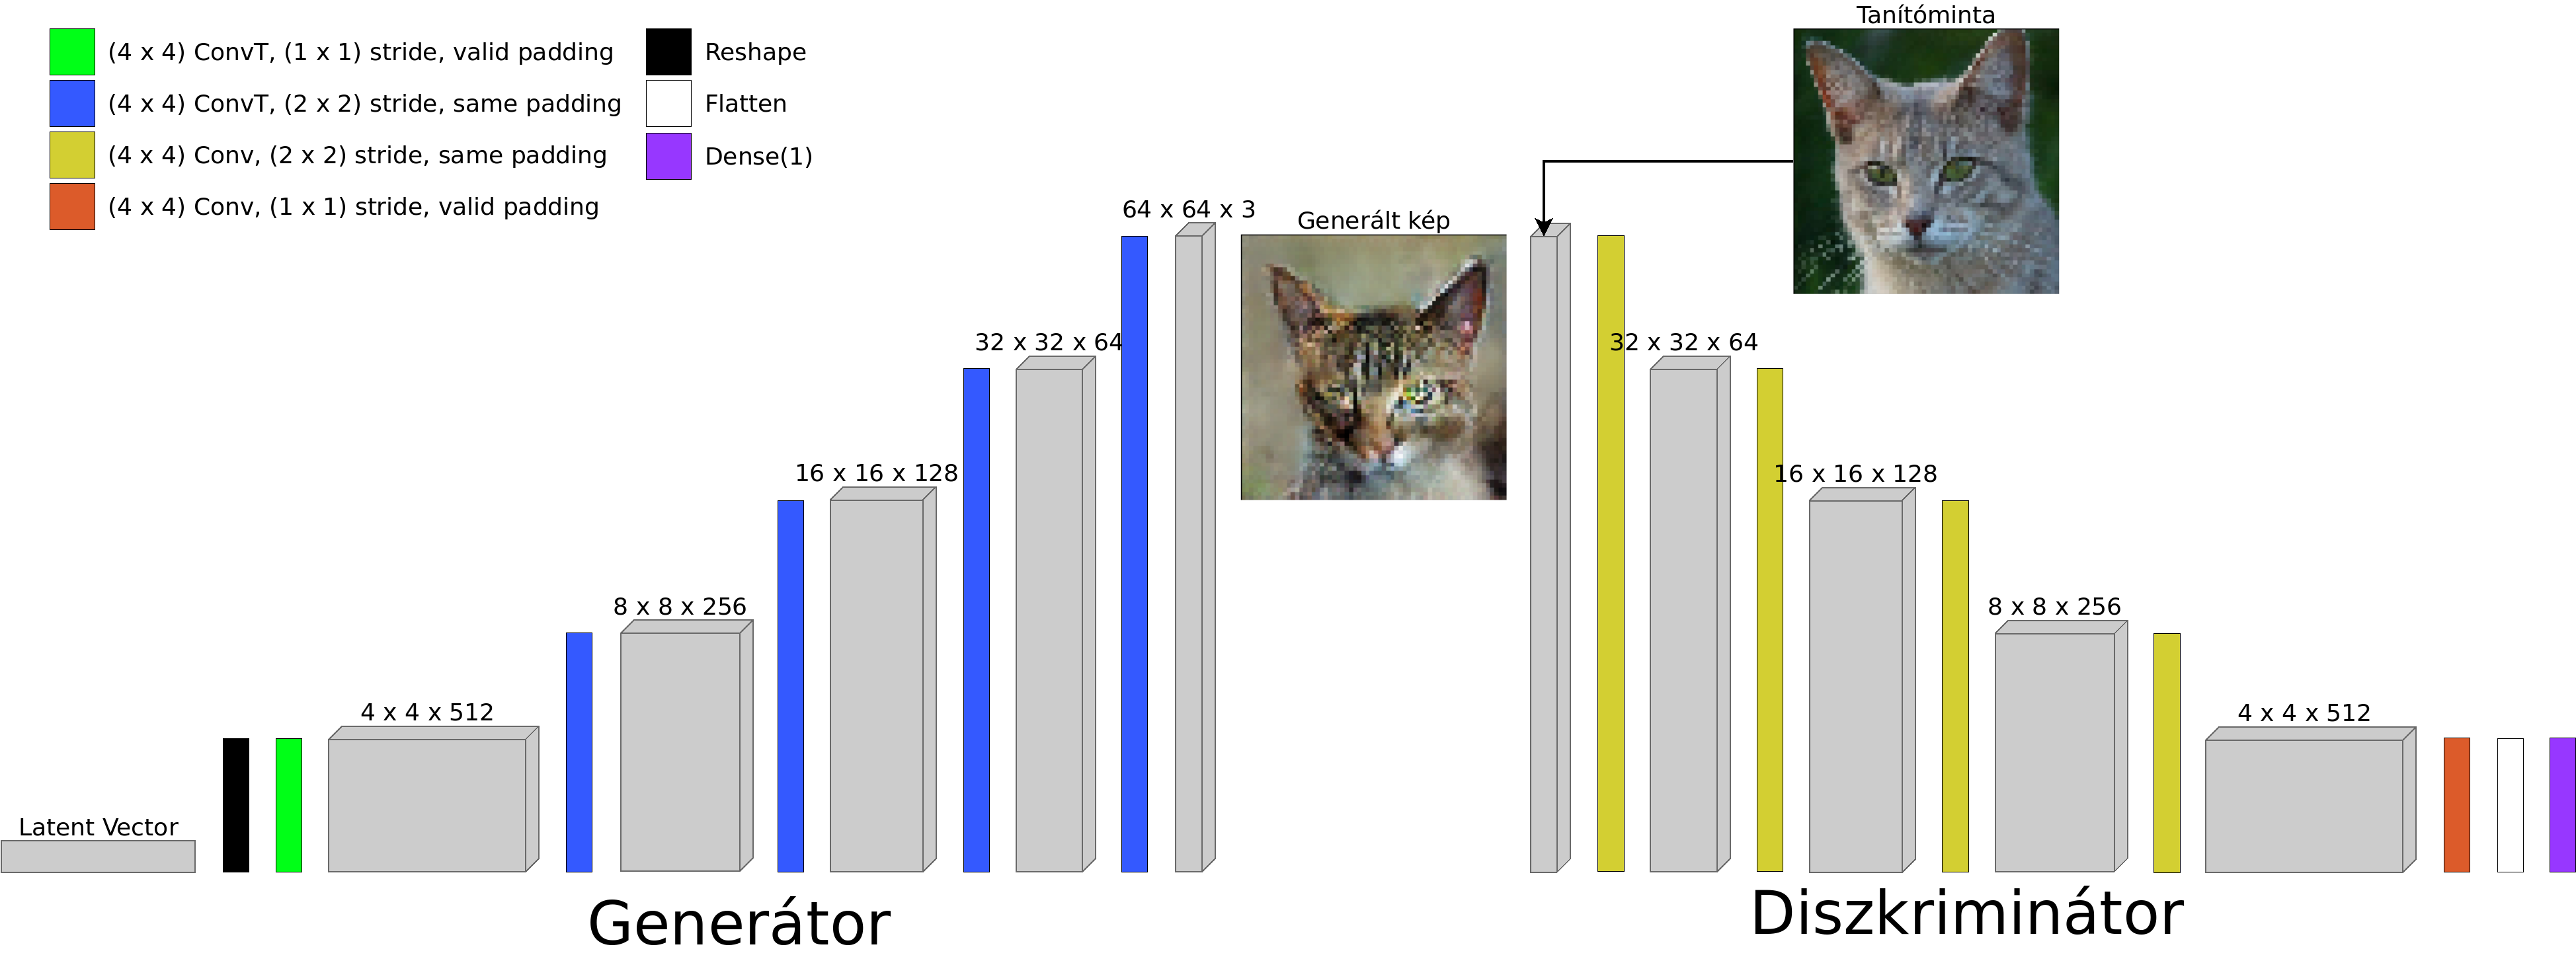
\includegraphics[width=15cm]{images/DCGAN.png}
\caption{DCGAN architektúra}
\label{fig:dcgan}
\end{figure}

\SubSection{Generátor}

Az osztályozáshoz használt konvolúciós hálókkal ellentétben a Generátorban a kisebb felbontás felől haladunk a nagyobb felbontásig.
A generátor modellem első implementációjában \textit{Dekonvolúciós} rétegeket alkalmaztam, amelyet \textit{Transzponált konvolúciós} rétegnek is nevezhetünk. A dekonvolúció a konvolúció ellentettje, vagyis a feladata, hogy egy alacsonyabb dimenziójú reprezentációt magasabb dimenzióba emeljen. Segítségével minden rejtett réteg kimenete egy nagyobb felbontású kép lesz. Tehát a hálónak jelen esetben meg kell tanulnia a rétegekben az optimális felbontás-növelést. Előre megadott paraméterek a filterek darabszáma, a kernel mérete, a strides és a padding. Ha a padding-et "same"-re és ha a strides paramétert $2 \times 2$-esnek választjuk, úgy a réteg kimenetén megjelenő kép felbontása dimenziónként kétszerese lesz a bemeneti oldalon megfigyelhető képnek. A rejtett rétegekben ReLU aktivációs függvényt (\ref{fig:relu}. ábra) használtam, a neuronok kezdő értékeit a He inicializációs technikával \cite{he2015delving} állítottam be.

\begin{figure}[h]
\centering
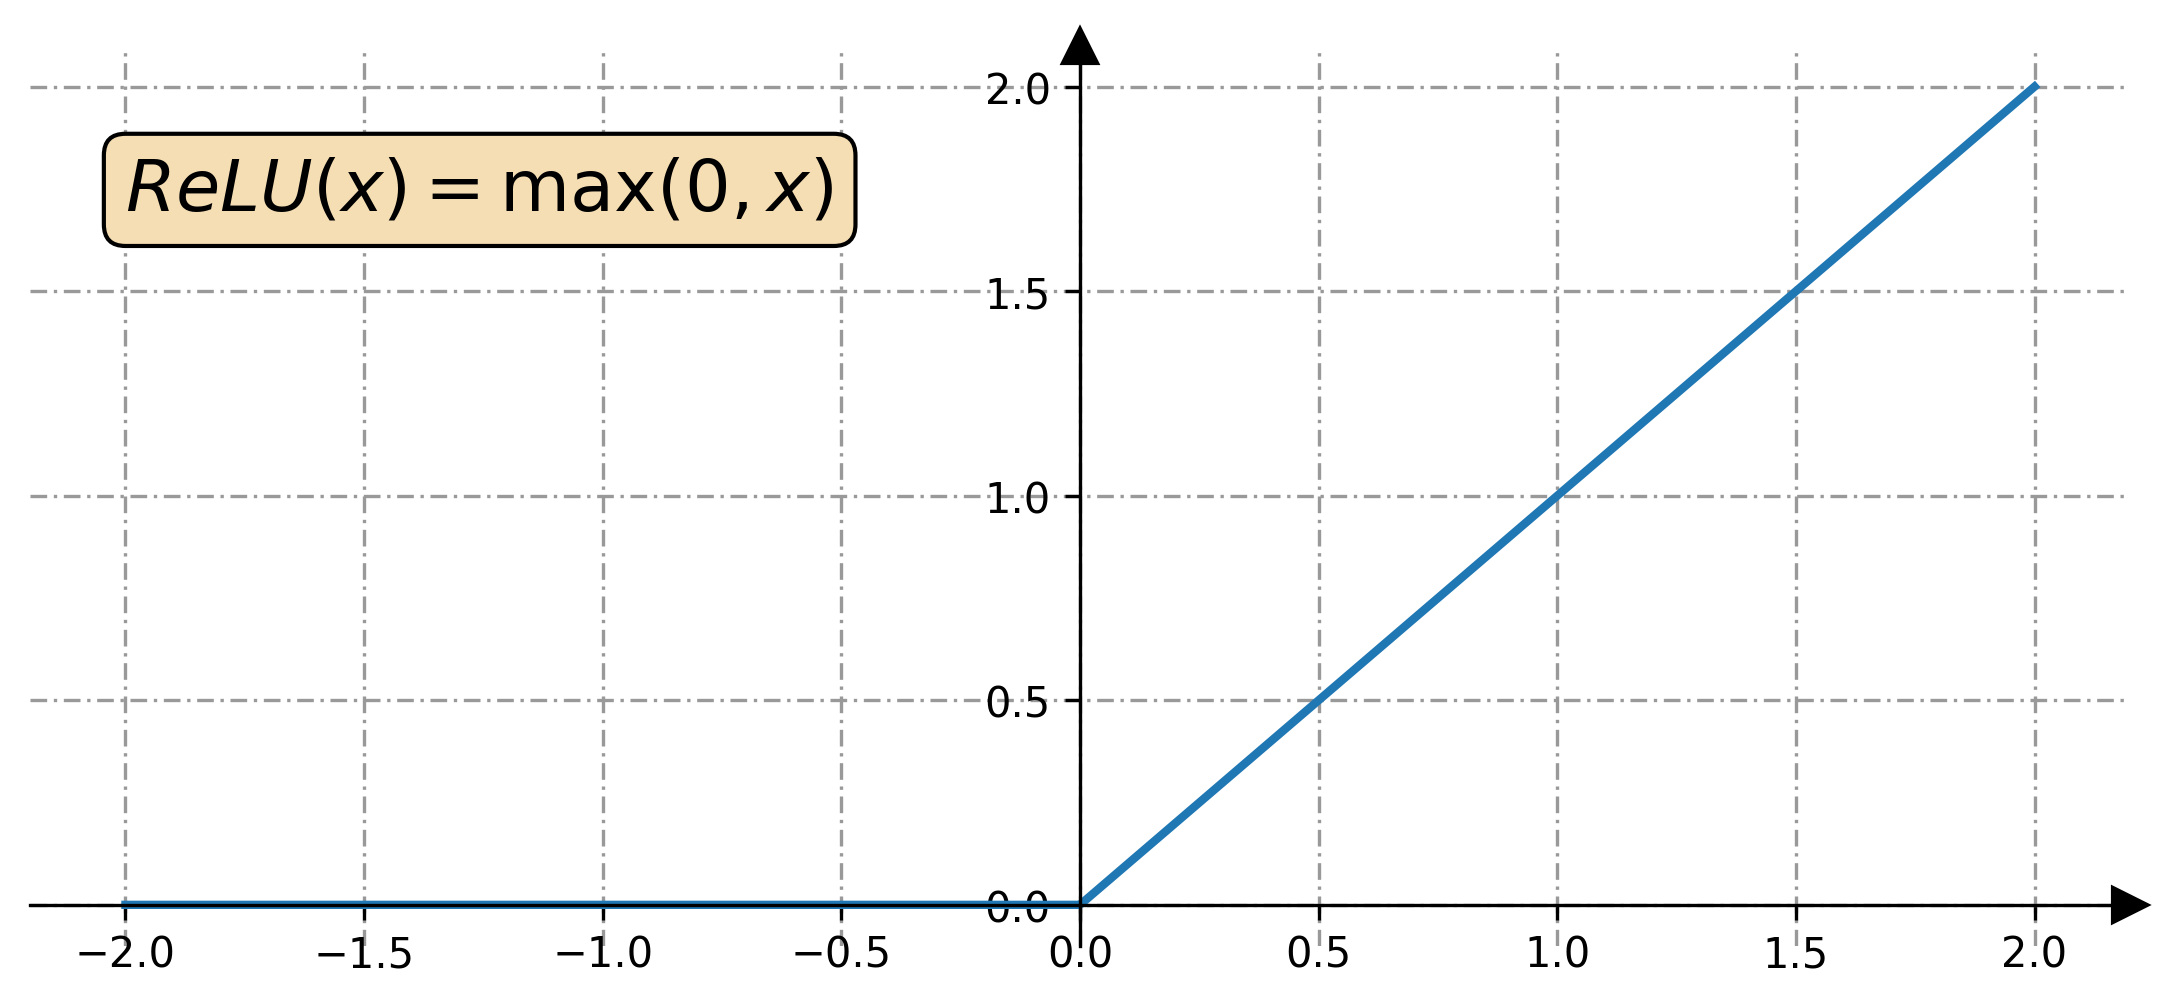
\includegraphics[width=10cm]{images/relu.png}
\caption{ReLU aktivációs függvény}
\label{fig:relu}
\end{figure}

A tanításhoz célszerű a kép pixeleinek intenzitását normalizálni a $[-1, 1]$ intervallumra lebegőpontos értékekre. A Generátor is ebben az intervallumban fogja a képek pixeleit generálni a hiperbolikus tangens kimeneti aktivációs függvényéből adódóan. A megjelenítéshez később természetesen denormalizálnunk kell a generált képek pixelértékeit a $[0, 255]$ tartományra.

A Generátor modell bemenetként az előre definiált látens tér dimenziójával megegyező dimenziójú zajt kap, vagyis annak a $z_n$ dimenziószámú térnek egy pontját. Majd ezen bemeneti zaj segítségével állítja össze a megfelelő kimeneti képet. A tanulás során tehát a látens tér tartományaihoz rendeli a tanult jellegzetességeket és a látens teret mintavételezve dekódolható a Generátor segítségével a ponthoz tartozó kép.

A bemeneti zaj egy \textit{Reshape} rétegen megy keresztül, amelyben a látens tér dimenziószámát átformázza egy $1 \times 1 \times z_n$ dimenziójú mátrixszá. Ezen réteg kimenetével a későbbi dekonvolúciós rétegek már tudnak dolgozni.
Ezután az első dekonvolúciós rétegen megy át a kapott mátrix, amely 512 darab filtert tartalmaz, $4 \times 4$-es kernelméretekkel dolgozik és 'valid' paddingot használ. Az aktivációs függvénye ReLU a már említett He inicializálással. Ezen lépés arra szolgál, hogy a látens térből előállítson egy $4 \times 4 \times 512$ alakú tensor-t, amely az első, legkisebb felbontású képünknek tekinthetjük ebben az esetben, ahol a színcsatornák száma 512 és a felbontása pedig $4 \times 4$.

A Generátorban ezután $2 \times 2$-es stride értékeket használva same padding-gel a kívánt felbontásig dekonvolúciós rétegeken keresztül növekszik a felbontás. A kernelméretét a rétegekben egységesen $4 \times 4$-ra állítottam be. Az aktivációs függvény szintén ReLU. A rétegekben haladva a filterek darabszáma pedig feleződik. A filterek optimális számára csupán csak empirikus eredményeket találtam a szakirodalomban. A felezéses eljárással a paraméterek száma viszonylag alacsonyabban tartható és a tanítás ideje is lecsökken.

A kimeneti képnek olyan tulajdonságokkal kell rendelkeznie, mint a tanítómintában szeplő képeknek. Például ha a tanítóminta színes képekből áll, \textit{RGB} színkeveréssel, vagyis három színcsatornával, úgy a Generátor kimenetén is ilyen képekre van szükségünk. Mivel az említett dekonvolúciós rétegek több mint 3 színcsatornával dolgoztak, a megjeleníthetőség miatt szükséges tehát az utolsó dekonvolúciós rétegben a 3 darab filter, amely egyaránt transzponálja az előző réteg reprezentációit az egyel magasabb felbontás értékbe, és a csatornák számát pedig 3-ra állítja.
Egyes GAN architektúrákban ez az utolsó réteg csupán a 3 színcsatornába vetítést végzi el konvolúciós réteggel és szokás \textit{toRGB} rétegnek is nevezni \cite{karras2017progressive, karras2019style, karnewar2020msg}. Viszont jelen esetben egyúttal a felbontást is növeli a példámban szereplő utolsó réteg, ha $1 \times 1$-es stride értékkel rendelkezne ez a dekonvolúciós réteg, akkor valójában úgy működne, mint egy konvolúciós réteg, és tényleg csak a csatornák számát változtatná meg. Viszont akkor szükség lenne még egy felbontásnövelő rétegre, amely tovább növelné a paraméterek számát.

Végül a hiperbolikus tangens aktivációs függvény (\ref{fig:tanh}. ábra) az eredményeket a $[-1, 1]$ intervallumba transzformálja.

Az alábbi kódrészletben látható a felvázolt generátor architektúra megvalósítása a Keras \textit{Sequential API}-ja segítségével.

\begin{python}
generator = keras.Sequential([
    keras.layers.Reshape((1, 1, 100), input_shape=[100]),
    keras.layers.Conv2DTranspose(512, (4, 4), (1, 1), "valid",
                                 activation="relu",
                                 kernel_initializer="he_normal"),
    keras.layers.Conv2DTranspose(256, (4, 4), (2, 2), "same",
                                 activation="relu",
                                 kernel_initializer="he_normal"),
    keras.layers.Conv2DTranspose(128, (4, 4), (2, 2), "same",
                                 activation="relu",
                                 kernel_initializer="he_normal"),
    keras.layers.Conv2DTranspose(64, (4, 4), (2, 2), "same",
                                 activation="relu",
                                 kernel_initializer="he_normal"),
    keras.layers.Conv2DTranspose(3, (4, 4), (2, 2), "same",
                                 activation="relu"),
    keras.layers.Activation("tanh")
])
\end{python}

\begin{figure}[h]
\centering
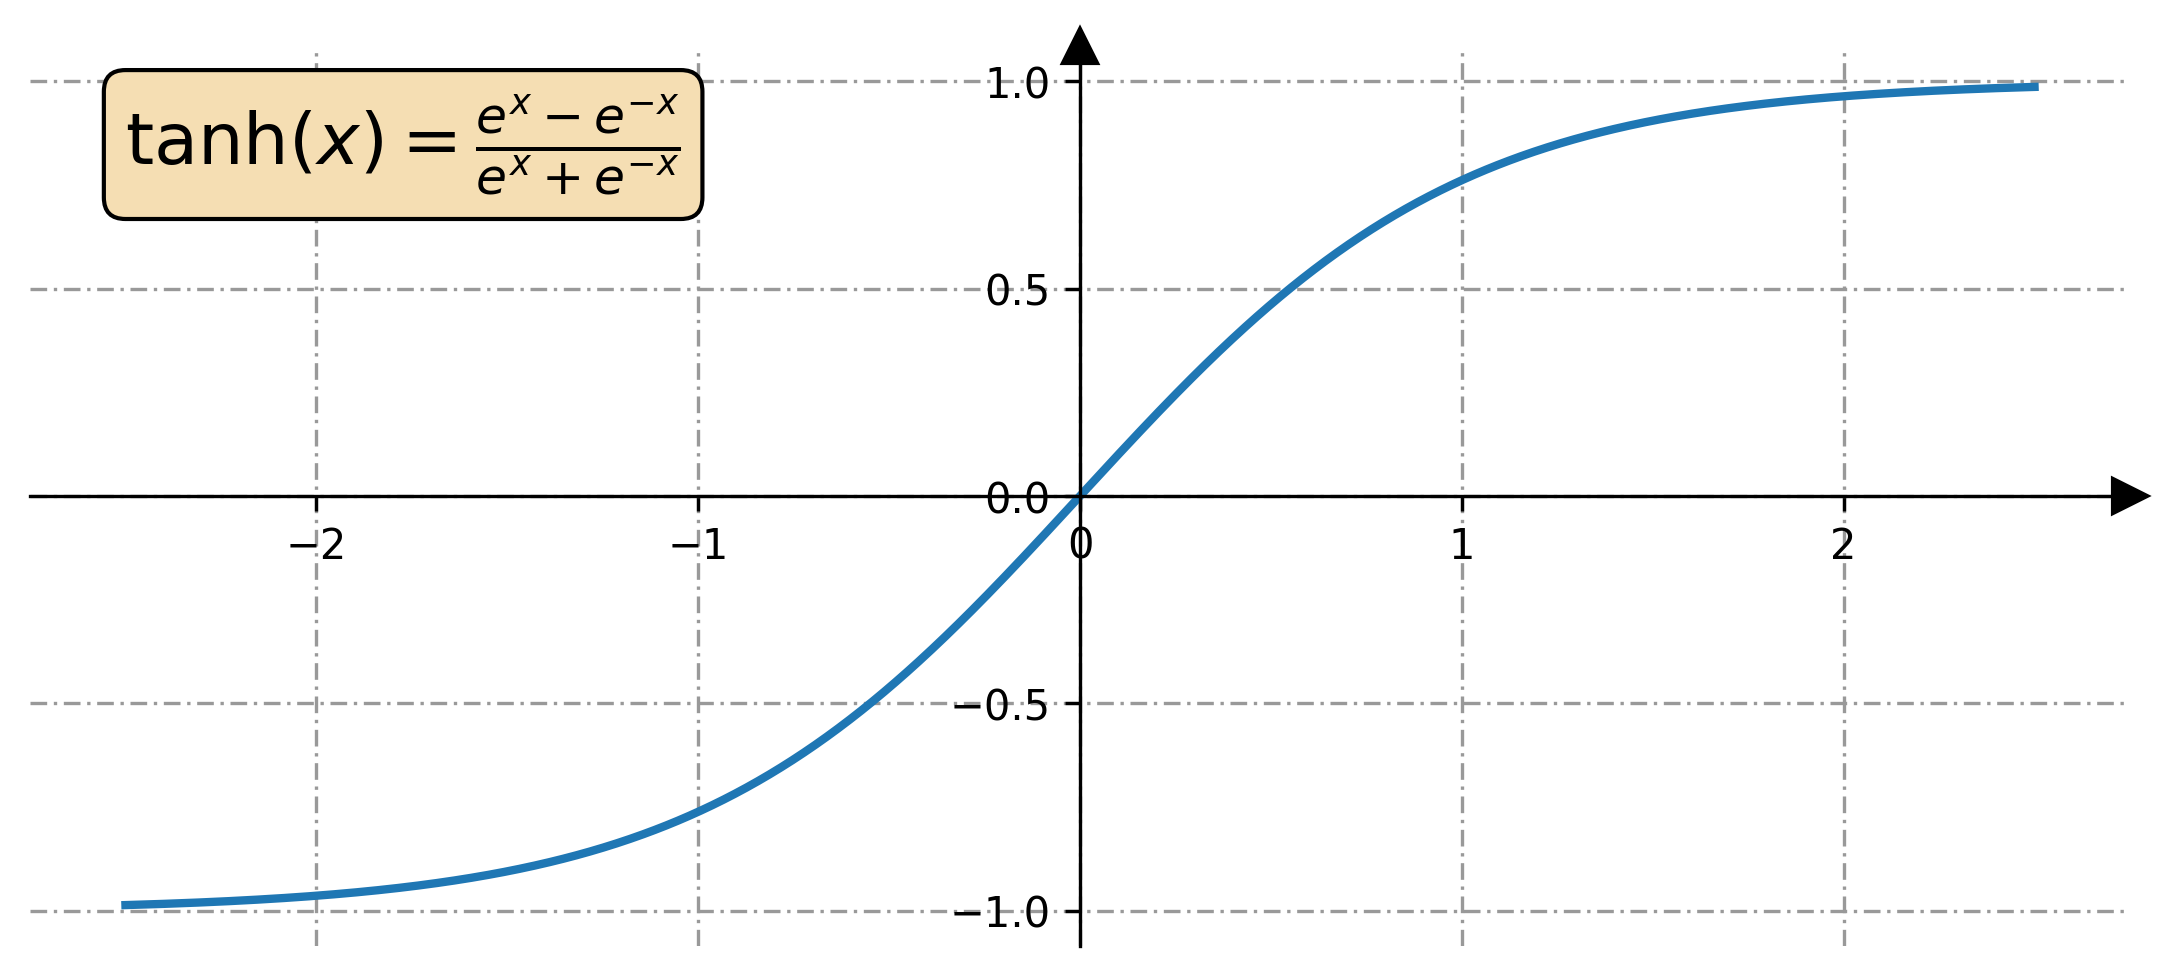
\includegraphics[width=10cm]{images/tanh.png}
\caption{Hiperbolikus tangens aktivációs függvény}
\label{fig:tanh}
\end{figure}

\SubSection{Diszkriminátor}

A Diszkriminátor modell lényegében egy bináris osztályozó, amely eldönti, hogy a bemenetül kapott kép valódi-e vagy hamis. A bemeneti kép konvolúciós rétegeken megy végig, kinyerve a jellegzetességeket és felállítva egy olyan belső reprezentációt, amely alapján az utolsó \textit{dense} réteg megfelelő kimenettel tud rendelkezni. A képen található mintázatokat a konvolúciós rétegek filterek segítségével tanulják meg, amelyek megadott kernelméretekben pásztázzák végig a bemenetet. Így az egyes konvolúciós rétegek kimeneteként egy olyan reprezentáció jön létre a bemeneti képről, amelyben érvényesülnek a pixeleket körülölelő további pixelek kapcsolatai is. Ezáltal az utolsó előtti réteg, a szerializáció (\textit{Flattening}) kevésbé fogja a kép tartalmára vonatkozó információt rontani. Mivel a tanítóminta képeinek pixelértékeit normalizáltuk a $[-1, 1]$ intervallumra, így a diszkriminátor a bemenetén is ilyen tulajdonságú képeket vár. A Diszkriminátor felépítésben hasonlít a Generátorhoz, lényegében annak tükörképeként képzelhetjük el. Viszont a dekonvolúciós rétegek helyett konvolúciós rétegeket alkalmazunk benne a jellegzetességek kinyerésére. Majd ha eljutunk a kívánt dimenziószámig, egy teljesen összekötött rétegben hozza meg a modell a döntést.

A generátorhoz hasonlóan az alábbi kódrészlet bemutatja a felvázolt diszkriminátor Keras Sequential API-val történő megvalósítását:
\begin{python}
discriminator = keras.Sequential([
    keras.layers.Conv2D(64, (4, 4), (2, 2), "same",
                        input_shape=(64, 64, 3), activation="relu",
                        kernel_initializer="he_normal"),
    keras.layers.Conv2D(128, (4, 4), (2, 2), "same", activation="relu",
                        kernel_initializer="he_normal"),
    keras.layers.Conv2D(256, (4, 4), (2, 2), "same", activation="relu",
                        kernel_initializer="he_normal"),
    keras.layers.Conv2D(512, (4, 4), (2, 2), "same", activation="relu",
                        kernel_initializer="he_normal"),
    keras.layers.Conv2D(100, (4, 4), (1, 1), "valid", activation="relu"),
    keras.layers.Flatten(),
    keras.layers.Dense(1)
])
\end{python}

Mint a kódrészletből is látható, az utolsó teljesen összekötött rétegnek nincsen aktivációs függvénye, \textit{Logits} kimenettel rendelkezik. A szigmoid függvényt a keresztentrópia számolásnál alkalmazzuk majd a dense réteg kimenetére.

\Aref{tab:gen_disc_params}. táblázatokban összefoglaltam az architektúra felépítését.

\begin{table}[h!]
	\centering
\caption{A hálózatokhoz tartozó rétegek és paramétereik}
\label{tab:gen_disc_params}
\medskip
\begin{tabular}{c c}
\scriptsize{
\begin{tabular}{@{\extracolsep{5pt}} |l c r| }
	\hline
	\multicolumn{3}{|c|}{\textbf{Generátor}} \\
	\hline
	Réteg & Aktivációs fv & Kimenet\\
	\cline{1-1} \cline{2-2} \cline{3-3}
	Input & - & (100)\\
	Reshape & - & (1, 1, 100)\\
	(4x4) ConvT & ReLU & (4, 4, 512)\\
	(4x4) ConvT & ReLU & (8, 8, 256)\\
	(4x4) ConvT & ReLU & (16, 16, 128)\\
	(4x4) ConvT & ReLU & (32, 32, 64)\\
	(4x4) ConvT & tanh & (64, 64, 3)\\
	\hline
	\multicolumn{3}{|r|}{Paraméterek száma: \textbf{3.5 millió}} \\
	\hline
\end{tabular}}

&\scriptsize{
\begin{tabular}{@{\extracolsep{5pt}} |l c r| }
	\hline
	\multicolumn{3}{|c|}{\textbf{Diszkriminátor}} \\
	\hline
	Réteg & Aktivációs fv & Kimenet\\
	\cline{1-1} \cline{2-2} \cline{3-3}
	Input & - & (64, 64, 3)\\
	(4x4)Conv & ReLU & (32, 32, 64)\\
	(4x4)Conv & ReLU & (16, 16, 128)\\
	(4x4)Conv & ReLU & (8, 8, 256)\\
	(4x4)Conv & ReLU & (4, 4, 512)\\
	(4x4)Conv & ReLU & (1, 1, 100)\\
	Flatten & - & (100)\\
	Dense(1) & - & (1)\\
	\hline
	\multicolumn{3}{|r|}{Paraméterek száma: \textbf{3.5 millió}} \\
	\hline
\end{tabular}}

\end{tabular}
\end{table}

\SubSection{Tanítás, mérések}

A felvázolt architektúrát az AFHQ dataset-en, Adam optimalizációs módszerrel, 0.0004 \textit{learning rate} hiperparaméter mellett tanítva a hibaértékek \aref{fig:mini-batch_loss_plot}. ábrához hasonlóan alakulnak.

\begin{figure}[h]
\centering
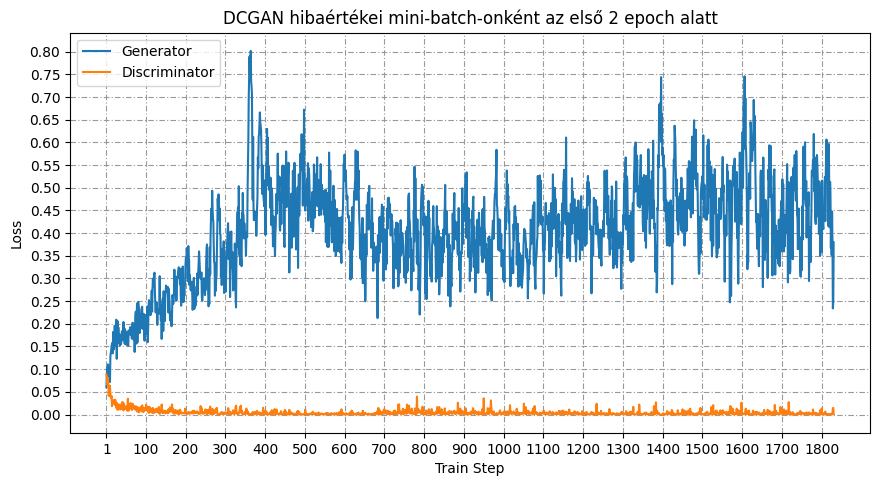
\includegraphics[width=15cm]{images/miniloss.png}
\caption{Hibaértékek mini-batch-enként}
\label{fig:mini-batch_loss_plot}
\end{figure}

Egy tanítási lépés egy mini-batch-en történő tanítást jelent, egy epoch pedig az összes mini-batch-en való tanítást jelenti.
Ha csak a nyers hibaértékre tekintünk, akkor azt figyelhetjük meg, hogy a tanítási lépések között erősen oszcillálnak az értékek. Kijelenthetjük a látott eredmények alapján, hogy a tanítás valóban nem stabil és látszólag tetszőlegesen módon változhatnak az értékek.
A szemléltetés kedvéért \aref{fig:epoch_loss_plot}. ábrán a mini-batch-eken számolt hibaértékek átlagait figyelhetjük meg epoch-onként.

\begin{figure}[h]
\centering
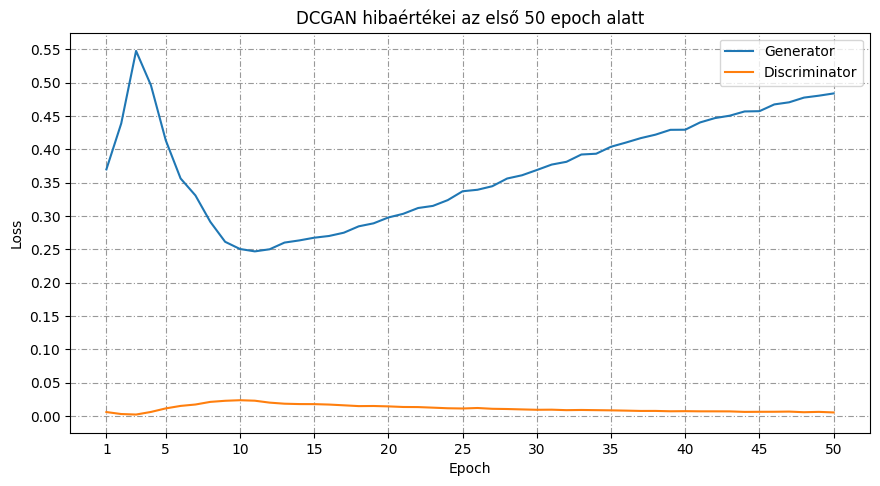
\includegraphics[width=15cm]{images/epochloss.png}
\caption{Hibaértékek epoch-onként}
\label{fig:epoch_loss_plot}
\end{figure}

Így simább görbéket kapunk, viszont erősen torzít az ábra, hiszen a GAN tanítási folyamata nem ilyen rendezett, mint ahogyan az első ábrán is láthattuk.
A hibaértékek változását vizsgálva megfigyelhető a versengés, vagyis hogy a két hálózat hibái mennyire ellentétesen mozognak az epoch-ok alatt. Mivel a tanulás során függőség van a két hálózat között, így ha a diszkriminátor egy vizsgált epoch alatt rosszabbul teljesítene a korábbi eredményekhez képest, akkor az a generátor javára válik és annak hibaértéke alacsonyabb lesz és fordítva. A generátor hibái többszörösek lehetnek a diszkriminátor hibáinak, de ez a jelenség teljesen természetes, hiszen a generátor lényegében a másik hálózat hibáiból tud csak tanulni, mivel a tanulás során nem látja a tanítóminta elemeit. A generátorban megfigyelhető, egyre növekvő hibaérték ellenére a generált képek minősége és részletezettsége is növekedni fog.

A hibaértékekből nem vonhatunk le pontos következtetéseket, így a fenti ábrák csupán szemléltetésképp készültek el. A GAN teljesítményének mérésére egyéb ajánlások jelentek meg, ilyen az \textit{Inception Score} \cite{salimans2016improved} és az \textit{Fréchet Inception Distance} \cite{heusel2017gans}.

\SubSection{Az architektúra gyengeségei, problémái}

A felvázolt architektúra tanítása során különféle problémák jelentkezhetnek, amelyek a végeredményt kisebb nagyobb mértékben ronthatják.

\begin{figure}[h]
	\centering
	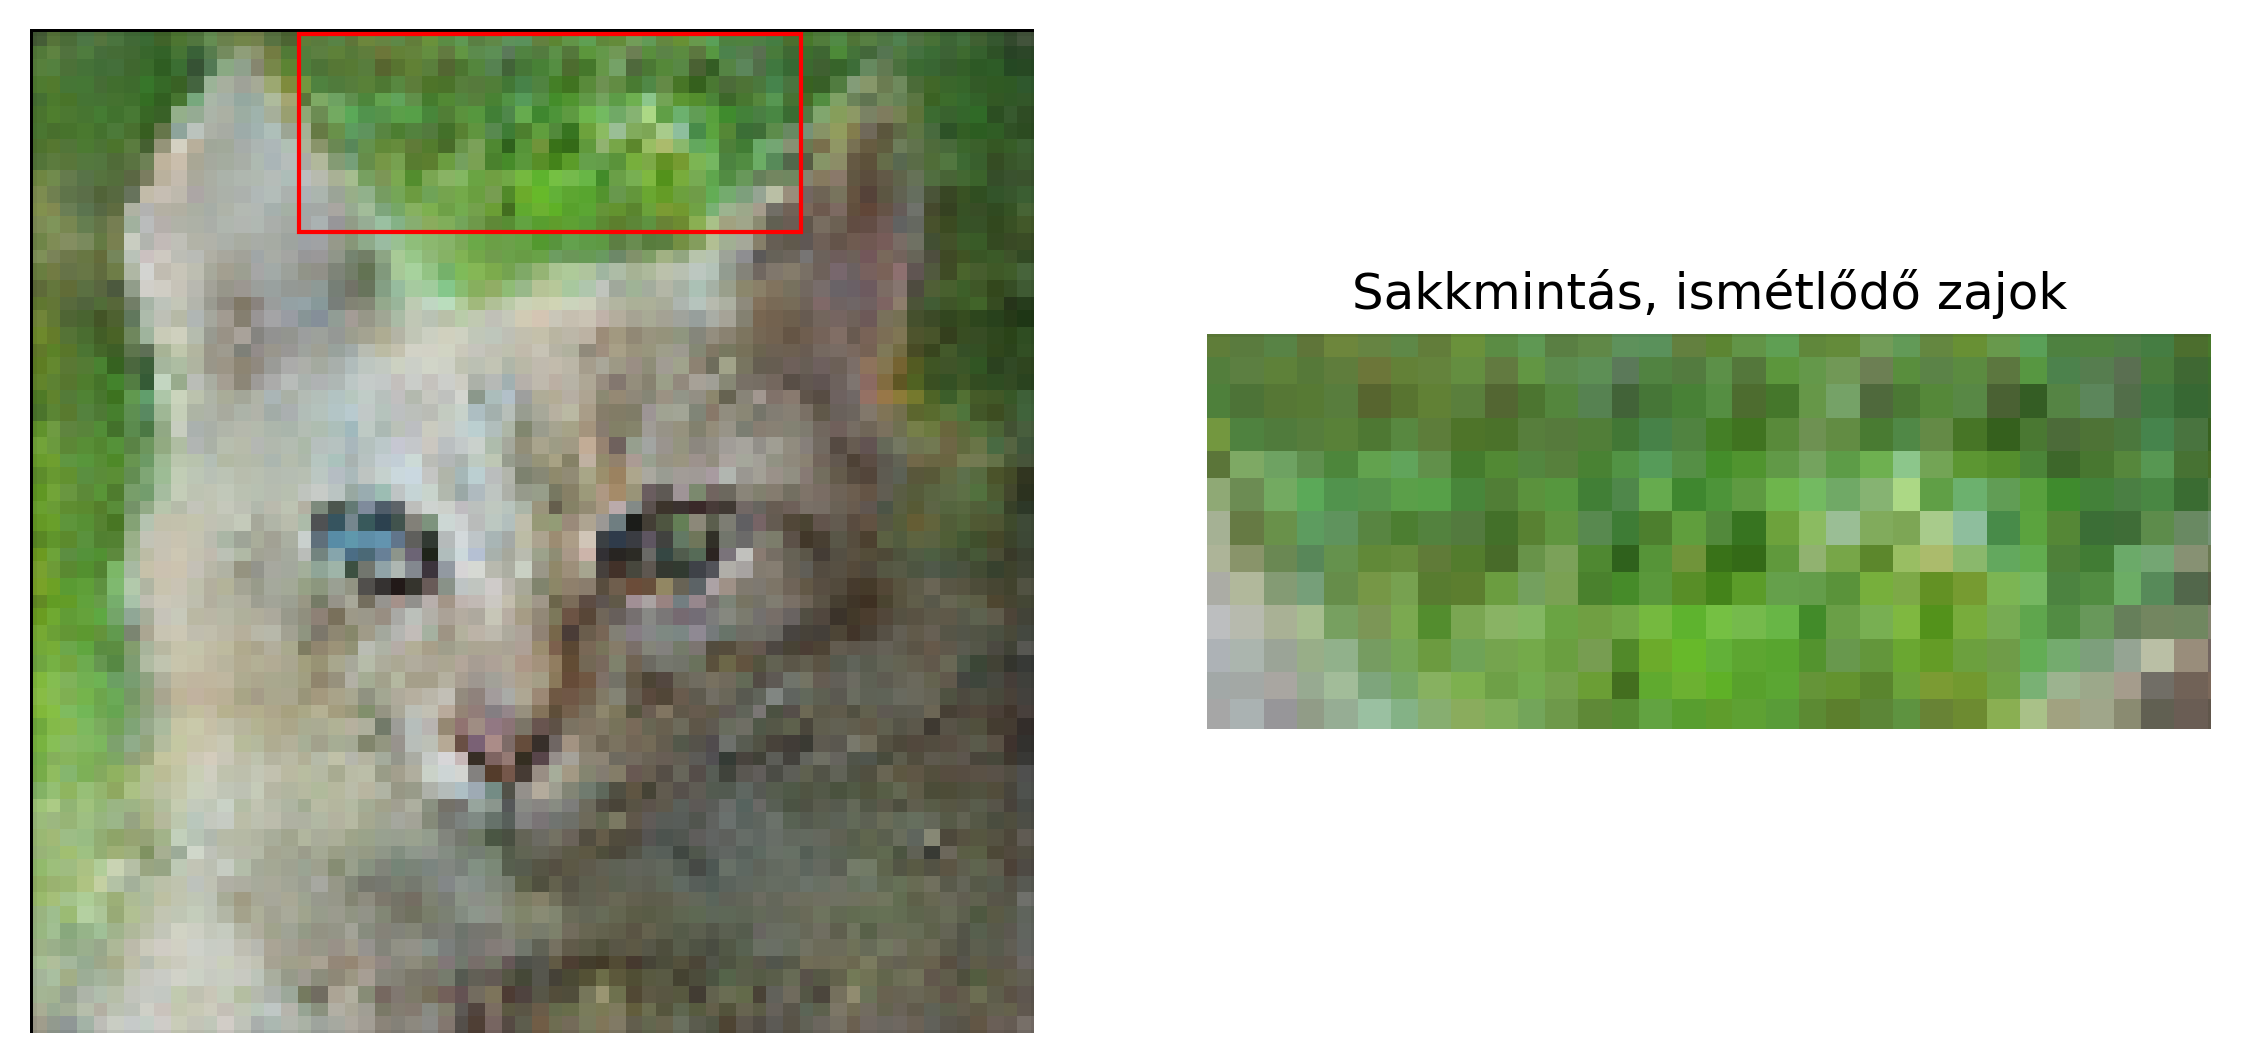
\includegraphics[width=13cm]{images/chessboard-patterns.png}
	\caption{Jellegzetes zajok a generált képeken}
	\label{fig:chessboard-patterns}
\end{figure}


\begin{itemize}
	\item A modell ebben a formájában igen hajlamos a \textit{mode collapse}-re, vagyis a tanulás során jelentkező összeomlásra. A jelenség és az elkerülésére irányuló néhány technika bemutatása a következőkben kerül ismertetésre.
	\item A konvolúciós rétegek működéséből adódóan csupán lokális pixel-környezetekre képes összefüggő részeket generálni a modell.\\
	Ez a működés alacsony felbontás mellett is anomáliákat idézhet elő, úgy mint a képeken megfigyelhető ismétlődő, sakktáblamintás zaj. Az említett zajra láthatunk példát \aref{fig:chessboard-patterns} ábrán. Megoldásként a Dekonvolúciós rétegek helyett a Konvolúciós és bilineáris interpolációval alkalmazott UpSampling rétegek használata javasolt \cite{odena2016deconvolution}.\\
	Ha a rejtett konvolúciós rétegek számával növelnénk a felbontást, akkor további nehézségbe is ütközünk: a modell nem lesz képes felismerni és megtanulni a tanítóminta képein megfigyelhető távoli, összefüggő tulajdonságokat. Így a generált képek részletezettsége alacsony lesz, gyakran \textit{blobokat} figyelhetünk meg csupán, különböző textúrákkal. \cite{salimans2016improved}
	
	\item A modellnek nincsen információja a különféle osztályokról, csupán a képek rendezetlen halmazán tanul, így magától kell megtanulnia a különféle osztályok jellegzetességeit.
	Az általánosítás szempontjából ez előnyös is lehet, viszont ha merőben különböző osztályokra szeretnénk betanítani a modellt, akkor az úgynevezett \textit{class conditoning} technika válhat a segítségünkre. A technikát a saját modellemre is kipróbáltam, a későbbiekben ismertetésre kerül.

\end{itemize}

\Section{GAN teljesítmény mérés}

A gépi tanulásos modellek tanítási életciklusának utolsó lépése optimális esetben a tesztelés. Hagyományos esetben a dataset-et három részre osztjuk fel: tanító-, teszt- és validáló halmazra. Hogy ezt milyen arányban tesszük meg, az függ a problémától is, de általánosan a teszt adathalmaz a dataset 20\%-a is lehet, a validáló halmaz még kisebb szelete a dataset-nek és a tanítóhalmazon történik a modell tanítása.
A teszt halmazt csupán egyetlen egyszer láthatja hagyományos esetben a modell, a tanítás után.
A teszthalmazzal szimuláljuk a modell valós adatokra történő alkalmazását, hiszen a modell számára ezen adatok teljesen ismeretlenek lesznek. A tesztadatok az eredeti dataset elemei, így rendelkezésünkre állnak az elvárt eredmények is, így a modell predikcióit össze tudjuk vetni az elvárt kimenettel, amelyből megbecsülhetjük a modell pontosságát különféle metrikák szerint.
A GAN esetében osztályozási feladatot a diszkriminátor lát el, viszont a hamis adatok nem részei a dataset-ünknek, azok a generátor által jöttek létre. A betanított modellnek csupán a generátora kerül felhasználásra, hiszen ezen komponens önmagában képes előállítani az új adatokat. A diszkriminátornak csupán a tanítás során van jelentősége és a validálásra önmagában nem alkalmas, hiszen ha a diszkriminátorunk rosszul tanult, úgy a generátorunk sem fog tudni a datasethez hasonló képeket generálni.
A GAN esetében nem szokás a dataset-et feldarabolni tanító és teszt részre, hiszen nem tudjuk a generátorra alkalmazni a már ismert metrikákat.
Ha képek generálása a feladat, úgy még nehezebb dolgunk van, hiszen a képeken hordozott információ igen összetett lehet.
A generátor kimenetét kell valamilyen módon tesztelnünk, ami nem egy egyértelmű feladat.
Egy emberi szemlélő természetesen meg tudná különböztetni a generált és a valós képeket. Lényegében a diszkriminátor feladatát látná el az emberi tesztelő, akinek hasonlóan mutathatnánk valódi és generált képeket, amelyekről el kell döntenie, hogy melyik a valódi és melyik a hamis. A fotórealisztikus képgenerálás igen nehéz feladat, és ha egy kicsit is rosszul teljesít a modell, azt egy emberi szemlélő hamar észreveszi és a modell pontossága igen alacsony lesz az emberi megfigyelő ítéletei alapján. Ha visszajelzést is kap az ember a hibáiról (Salimas et al. \cite{salimans2016improved}), akkor a továbbiakban sokkal pesszimistább ítéletet hoznak a tesztelők a képekre. Bináris, osztályozás helyett diszkrét vagy folytonos skálán is mérhetnénk a generált képeink jóságát. A pontos mérési eredmények érdekében több résztvevőt is be kellene vonnunk a tesztelésbe. Már belegondolva is igen lassú és költséges feladat lenne a modellünk tesztelése, így nem hagyatkozhatunk az emberi validálásra. Ez motiválta Salimas et al.-t is.

Az alábbi két ajánlás két mérőszámot definiál, amelyek segítségével meghatározhatjuk a GAN modellünk teljesítményét. Ezen validálási technikák megjelenése óta az újonnan megjelent GAN architektúrák mindegyikét lemérték és a GAN-al foglalkozó cikkekben táblázatokban vetik össze a különféle modellek teljesítményét a sajátjukkal.
A két mérőszámot együttesen szokták alkalmazni, hiszen egyik módszer sem tökéletes, viszont a kettőt együtt alkalmazva ad egy bizonyos képet a modellünk teljesítményéről.
A két mérőszám közös jellemzője, hogy mindkettő az Inception modell által kinyert jellegvektorok alapján határozza meg a modell jóságát.

Az alábbi kódrészlet az ImageNet adathalmazon betanított Inception modell használatát kívánja szemléltetni Keras segítségével. A kódrészlet első futtatásakor a modell súlyai letöltésre kerülnek és a további betöltés esetén egyből rendelkezésre fog állni.

\begin{python}
inception_model = keras.applications.InceptionV3(weights="imagenet")
predictions = inception_model.predict(images)
\end{python}

Az Inception modell bemenete alapértelmezett beállítások mellett egy $299 \times 299$ -es felbontású RGB színcsatornákkal rendelkező kép. A pixelértékeket normalizáltan várja a modell a $[-1, 1]$ tartományon. A modell inicializálásakor paraméterként megadhatjuk a bemenet méretét, viszont az nem lehet $75 \times 75$-nél kisebb. Ha az \texttt{include\_top} paramétert \texttt{True} értékkel állítjuk be, úgy a modell tartalmazni fogja az utolsó Dense rétegét is, amely az ImageNet súlyok alapján betanított modell esetében 1000 osztály detektálására lesz képes.

Az említett, GAN teljesítménymérésére használatos módszerek az \textit{Inception Score} (IS) és \textit{Fréchet Inception Distance} (FID). Ezeket kívánom bemutatni az alábbi két alfejezetben.

\SubSection{Inception Score}
Az Inception Score \cite{salimans2016improved} technikát Salimans et al. az emberi tesztelés kiváltására vetette fel. A méréseik alapján a technika sok minta figyelembevételével igen jól közelíti az emberi tesztelők által mért eredményeket.
Alapjául az Inception model szolgál, amelyet az ImageNet dataset-en tanítottak be. Minden egyes generált képet beadnak inputként a betanított Inception modellnek, hogy megkapják a conditional label eloszlást, ami tehát $p(y|x)$. Az olyan képeken, amelyeken jelentőségteljes objektumok figyelhetők meg, alacsony entrópiájú $p(y|x)$-el kell rendelkeznie. Vagyis a generált képen minél kevesebb objektumot kell felismernie a modellnek.
Továbbá az is lényeges szempont, hogy a generátor különféle képeket generálon, így a következőnek magas entrópiával kell rendelkeznie:
$$ \int \! p(y|x = G(z)) \; \mathrm{d}z. $$
Az Inception Score tehát:
$$ \exp(\mathbb{E}_x KL(p(y|x)||p(y))).$$
Minél magasabb ez a szám, annál jobbnak tekinthető a GAN teljesítménye.

Az Inception Score hivatalos implementációja\footnote{Az Inception Score hivatalos implementációja: \url{https://github.com/openai/improved-gan/tree/master/inception\_score}.} még a TensorFlow 1-es verziójában lett megírva, viszont a 2-es verzióval futtatva is működésre lehet bírni a megfelelő importok alkalmazása mellett. A méréshez a kigenerált képekre lesz szükségünk. A dolgozatom modelljeinek méréséhez a generált képek NumPy tömbökben kerültek kimentésre. %TODO: Notebookok behivatkozása

\SubSection{Fréchet Inception Distance}
Az Incepton Score kiegészítésére megjelent egy másik, széles körben elfogadott teljesítménymerő technika, a Fréchet Inception Distance (FID) \cite{heusel2017gans}. Az IS nem vette figyelembe a tanítóminta statisztikáit, és ez egy igen nagy hátránya a technikának. Továbbá az IS feltételein is javítottak, hogy a mintákon megtalálható zajok is befolyásolják a végső eredményt. Az FID számolásnál az Inception modell utolsó rejtett rétegének kimenetét veszik figyelembe, amely 2048 elemű jellegvektort jelent. A mérés elvégzése előtt a GAN modell tanításához használt adathalmazon kell vizsgálatot végezni, majd a generált képek kerülnek vizsgálatra, és az így kapott értékek alapján kapjuk meg a távolságot.

A számítási mód az alábbi formában adható meg:
$$ d^2((\boldsymbol{m}, \boldsymbol{C}), (\boldsymbol{m}_w, \boldsymbol{C}_w)) = \|\boldsymbol{m} - \boldsymbol{m}_w \|_2^2 + Tr(\boldsymbol{C} + \boldsymbol{C}_w - 2(\boldsymbol{C}\boldsymbol{C}_w)^{\frac{1}{2}}) $$
Minél alacsonyabb az FID, annál jobb a modell teljesítménye az adott tanítómintán.

Az FID hivatalos implementációja\footnote{A Fréchet Inception Distance hivatalos implementációja: \url{https://github.com/bioinf-jku/TTUR}.} szintén TensorFlow 1-ben került megvalósításra.

\Section{Mode collapse jelenség}

A \textit{Mode collapse} jelenség alatt a tanulás során bekövetkező azon anomáliát értjük, amely során a Generátor a látens tér bármely pontjára ugyanolyan kimeneti képet generál. A képek között minimális változatosság ugyan megfigyelhető, viszont a minőségük erősen romlik ilyen esetben. Előfordulhatnak olyan esetek is, amikor egy-egy megtanult képi jellegzetességek jelennek meg a kigenerált képeken teljesen indokolatlanul, és ezen jellegek helyére kerülnek újak a további tanítási lépések alatt. A tanítás közben felléphetnek lokális mode-collapse-ok is, amelyek a látens-tér egyes tartományaiban alakulhatnak ki \cite{zhang2018stackgan++}. \Aref{fig:mode-collapse}. ábrán láthatunk néhány példát a problémára.

\begin{figure}[h]
	\centering
	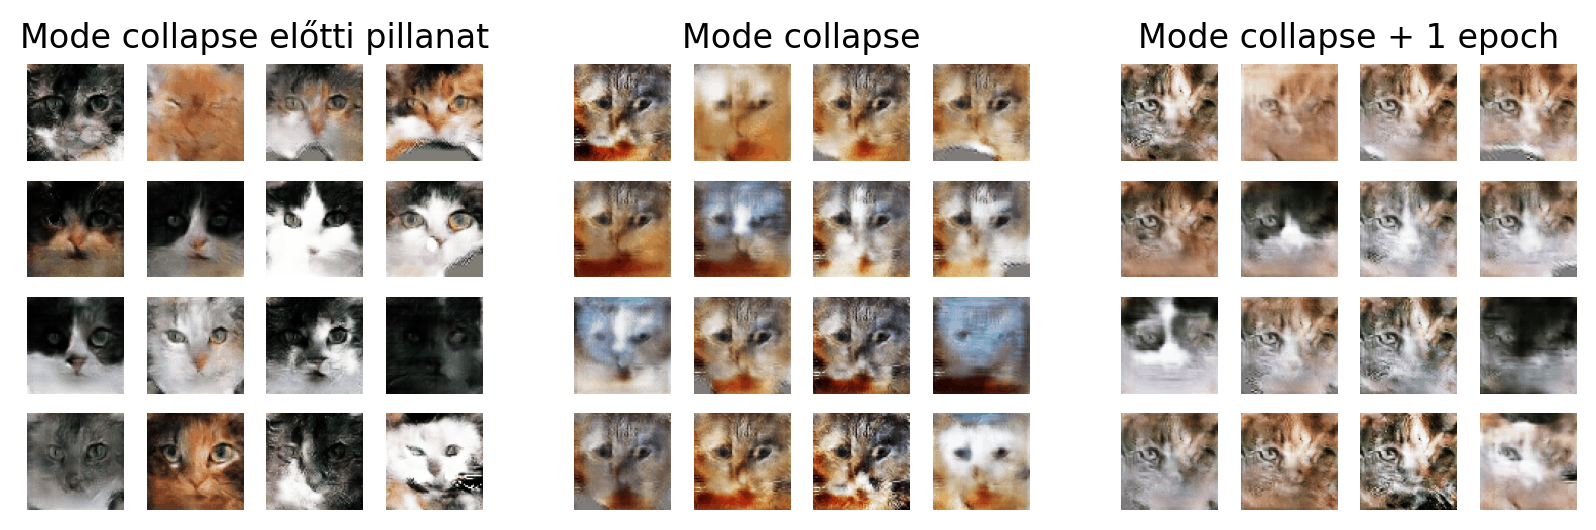
\includegraphics[width=15cm]{images/mode-collapse.png}
	\caption{Mode collapse jelensége}
	\label{fig:mode-collapse}
\end{figure}

Ez a jelenség valójában tekinthető egyfajta \textit{overfitting}-nek is, vagyis túltanulásnak, hiszen a Generátor úgy tudja átverni a Diszkriminátort, hogy közben a modell használhatatlan lesz. Viszont a mode-collapse elnevezés találóbb, hiszen amikor ez bekövetkezik, akkor a további tanítási lépések során úgy tűnhet, hogy stablinak tűnő modell hirtelen összeomlott volna.
A mode-collapse fellépése esetén a model további tanítása során minden egyes epoch-al változik a mode, vagyis az előzőtől eltérő kép jelenik meg a kimeneten (szintén minden egyes mintavételezett pontra hasonló). Mivel a diszkriminátor a mini-batch minden egyes bemenetét egymástól függetlenül dolgozza fel, így a gradienseiben sem jelenik meg olyan információ, amely a generátort változatosabb képek generálására bíztatná. A mode collapse esetén a diszkriminátor egyetlen pontot képes csak valódi adatnak tekinteni, majd minden egyes frissítéssel a pont elmozdul, ezzel magyarázható, hogy az összeomlás után tanítva minden egyes iterációval változik ezen pont, amire \textit{mode}-ként szokás hivatkozni \cite{salimans2016improved}. A GAN modellünk ezáltal használhatatlanná válik.

Egyes szerzők munkájában kiemelik, hogy az összeomlásig tanítják a felvázolt modelleket, és az összeomlás előtti állapotokra állítják vissza a hálózat súlyait a használathoz, mint például a BIG-GAN architektúra esetében is \cite{brock2018large}.

\begin{figure}[h]
	\centering
	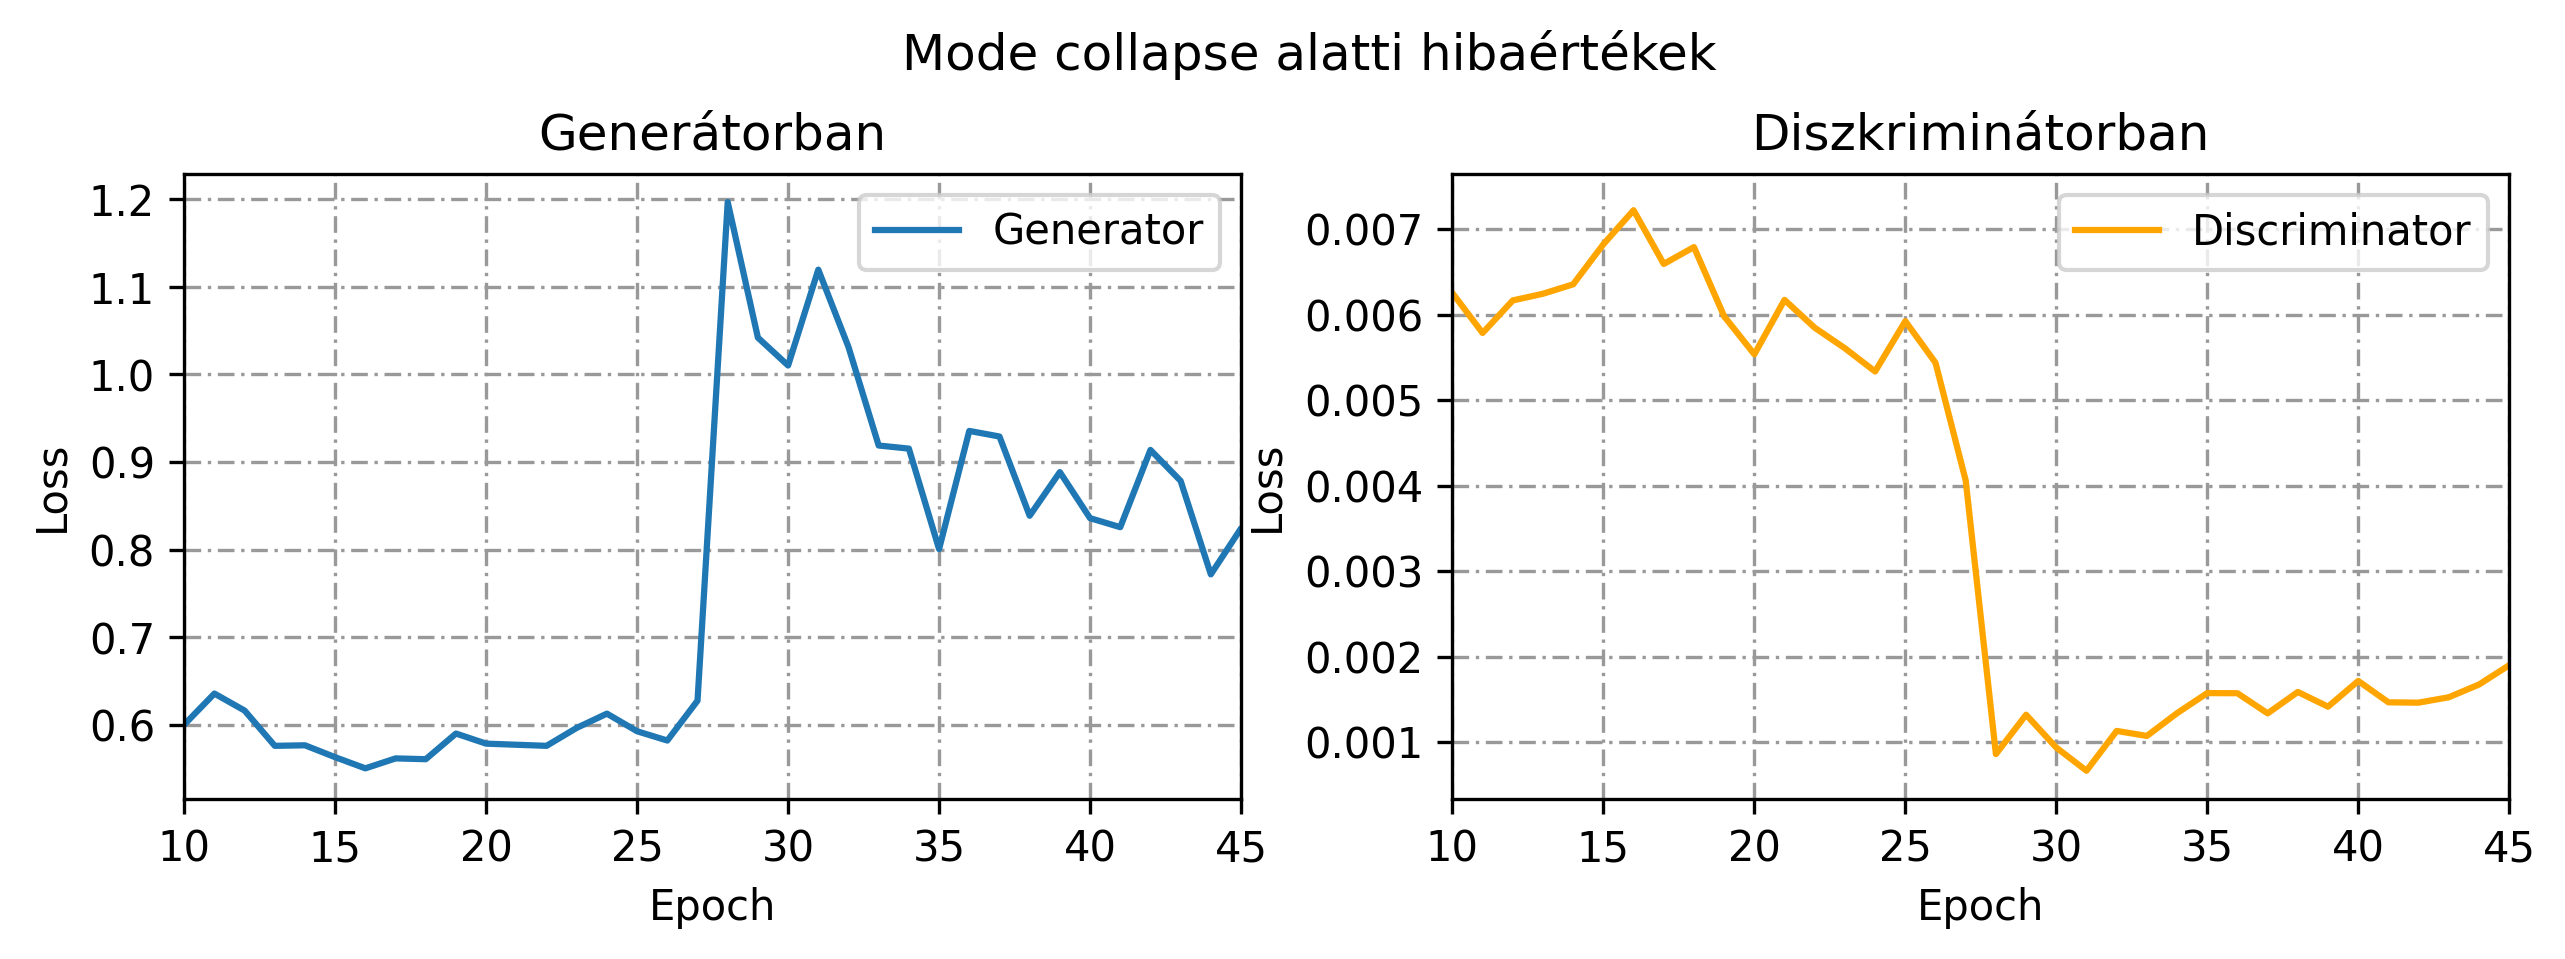
\includegraphics[width=15cm]{images/mode_collapse_loss.png}
	\caption{Mode collapse pillanata a hibagörbéken}
	\label{fig:mode_collapse_loss}
\end{figure}

\Aref{fig:mode_collapse_loss}. ábrán megfigyelhető a Generátor és a Diszkriminátor hibáinak alakulása a tanulás alatt. A kiugró hibaérték mindkét háló esetében ugyanazon epoch alatt jelentkeztek és a kimeneti képeket megvizsgálva megfigyelhetjük, hogy a modell valóban mode collapse áldozatává vált. Az ábrán azt is megfigyelhetjük, hogy a tanítás egészen korai szakaszában jelentkezett ezen anomália. Ennek oka az, hogy egy olyan adathalmazon tanítottam a modellt, amelyen semmiféle tisztítást nem alkalmaztak. Az adathalmaz a \textit{Flickr30k} \cite{young2014image}, amely egy ingyenes internetes képmegosztó weboldalról összegyűjtött képekből áll és 30 ezer képet tartalmaz. A képekhez leíró mondatok is tartoznak, amelyeket a tanítás során nem vettem figyelembe. Ilyen véletlenszerű és változatos képekre a modell jelenlegi formájában nem képes általánosítást találni, így a megfelelően előkészített adathalmaz továbbra is igen fontos része a GAN megfelelő tanításához.

A mode-collapse detektálása abban az esetben történhet a hibafüggvények vizsgálatával, ha a modellben teljes összeomlás figyelhető meg. A kisebb, lokális mode-collapse-ek esetében nem kapunk ilyen visszajelzést a hibafüggvényektől. A detektálásra alkalmasak lehetnek a validálási/teljesítménymérő módszerek is, vagyis az előbbiekben ismertetett IS és FID módszerek, amelyek a kigenerált képek változatosságát is figyelembe veszik az értékelés során.

\Section{Regularizációs módszerek}

A GAN tanítása során nehézségekbe ütközhetünk. Legrosszabb esetben nem is kezd el konvergálni a generátor kimenete a tanítóminta képeihez, viszont abban az esetben gyanakodhatunk, hogy a modellünk nem lett helyesen felépítve. Amennyiben mégis elkezd fejlődni a modell, és nem csak zaj jelenik meg a kimeneten az egyes tanítólépések után, de bizonyos számú epoch után mode collapse lép fel, úgy fontolóra vehetjük a következő regularizációs technikákat.

\SubSection{Label-smoothing}

A \textit{label-smoothing} az egyik legegyszerűbb regularizációs trükk, amely a neurális hálók overfitting problémáját kívánja kiküszöbölni. Ezen módszer alkalmazásához nem szükséges módosítanunk az architektúránkat, csupán a hibafüggvényt, így ez egy egészen egyszerűen implementálható technika. GAN esetében a diszkriminátor hibafüggvényét szokás módosítani oly módon, hogy a bináris keresztentrópia számolás során a valós bemeneti képek 1-es címke helyett valamennyivel alacsonyabb értéket, például 0.9-et kapnak. Ezzel a beállítással a diszkriminátor kevésbé lesz hajlamos a túlzott magabiztosságra a valós bemeneti képek esetén, teret adva a generátor fejlődésének. Ennek megvalósítása a következő Python kódrészletben látható.

\begin{python}
	def discriminator_loss(real_output, fake_output):
	real_loss = cross_entropy(
	tf.constant(np.full(real_output.shape, 0.9)),
	real_output)
	fake_loss = cross_entropy(
	tf.constant(np.full(fake_output.shape, 0)),
	fake_output)
	total_loss = real_loss + fake_loss
	return total_loss
\end{python}

A regularizációs technikákban megfigyelhető néhány esetben egy kicsi ellentmondásosság is, például egyes technikák a diszkriminátort hátráltatják, míg mások a generátor dolgát nehezítik meg. Természetesen a problémától függ, hogy melyik módszer alkalmazható egy adott modellnél.


\SubSection{Megfelelő inicializációs stratégia}

A mély neurális hálózatoknál igen gyakran előforduló probléma az úgynevezett exploding vagy éppen a vanishing gradiensek jelensége, amelyet gyakran csupán instabil gradienseknek is szokás nevezni \cite{geron2019hands}.
A tanítás forward-propagation stádiumában a hálózat kimenetén megfigyelhető túl magas vagy éppen túl alacsony értékek a hibafüggvény meghatározásánál is szélsőséges értékeket okozhatnak.
A backpropagation stádiumában az output rétegtől haladunk az input felé, amely során kiszámolásra kerülnek a gradiensek a hálózat minden egyes paraméterének függvényében, majd Gradient Descent vagy ahhoz hasonló algoritmus segítségével frissülnek a hálózat paraméterei. Mindkét irányban fontos lenne elkerülni az esetleges kilengéseket, hogy a tanítás stabilitását elősegítsük.
Az olyan hálózatoknál, amelyekben több rejtett réteg is található, az instabil gradiensek jelensége még inkább érvényesül. A backpropagation során az input réteg felé haladva a gradiensek hajlamosak lehetnek igen kis értékekre zsugorodni. Ilyen esetben az alacsonyabb rétegek rendszerint lassabban fognak tanulni, amely szintén komoly problémát jelent.
A hálózat rétegeiben megtalálható neuronok az előző rétegek neuronjaitól függenek, illetve a kimenetük a következő réteg neuronjait is befolyásolja. Egy esetlegesen fellépő túl magas vagy túl alacsony kilengés a kimeneti értékekben komoly hatással lehet a teljes hálózatra.

Az instabil gradiensek megelőzésére az egyik irány a neuronok inicializációs stratégiájának megválasztása.
Az évek során több ajánlás is érkezett, a különböző felépítésű hálózatokra különböző technikák váltak be.

Kiemelnék két inicializációs technikát, a Glorot \cite{glorot2010understanding} és a He \cite{he2015delving} stratégiákat, amelyek széleskörűen alkalmazhatónak bizonyultak.
A kezdőértékek generálásához figyelembe veszik a rétegek be- és kimeneti kapcsolatainak számát is, amelyet $fan_{in}$ és $fan_{out}$-nak is nevezhetünk és azok átlagát használják fel a számoláshoz:
$$fan_{avg} = \frac{fan_{in} + fan_{out}}{2}.$$

A \textit{Glorot/Xavier} inicializációs stratégia normális és egyenletes eloszlásra is számolható.
Normális eloszlás esetén a várható értéket $m = 0$-ra kell választani, a szórásnégyzet pedig: $ \sigma^2 = \frac{1}{fan_{avg}} $, tehát
$$ \mathcal{N}\left(0, \frac{1}{fan_{avg}}\right). $$
Egyenletes eloszlás esetén $\pm r$ között (vagyis $ \mathcal{U}\left[-r, r\right] $):
$$r = \sqrt{\frac{3}{fan_{avg}}}.$$

Ezen inicializációs stratégia a tangens-hiperbolikusz, logisztikus és softmax aktivációs függvényekkel rendelkező rétegekben használatosak. 

A \textit{He/Kaiming} inicializáció hasonló megközelítést alkalmaz.
Normális eloszlásra:
$$ \mathcal{N}\left(0, \frac{2}{fan_{in}}\right), $$
Egyenletes eloszlásra ($ \mathcal{U}\left[-r, r\right] $):
$$r = \sqrt{3 \cdot \frac{2}{fan_{in}}}.$$

Ezen inicializációs stratégia pedig a ReLU aktivációs függvények családjával rendelkező rétegekben ajánlott használni.

A Keras a Glorot inicializálást használja alapértelmezetten.

\SubSection{Batch Normalization}

Az instabil gradiensek problémája a tanítás során is jelentkezhet. A megfelelő inicializációs stratégia nem garantálja a teljes stabilitást, csupán egy kezdeti optimális állapotot biztosít a modellnek.
Az input adatok standardizálása áll a Batch Normalization technika mögött, amelyet a rétegek között vagy a rétegek aktivációs függvénye előtt ajánlott megtenni. A Batch Normalization technika alkalmazásához tehát minimálisan módosítanunk kell a meglévő modelljeink architektúráját. Azt figyeltem meg, hogy ezen technika alkalmazása teljesen empirikus módon történik és nincsen egy általánosan elfogadott módszer arra sem, hogy pontosan hol kell elhelyezni a réteget: az aktivációs függvények előtt vagy után. Kétségtelen, hogy a technika alkalmazásával stabilabb tanítást eredményez és széleskörűen alkalmazható a mély neurális hálózatokban.

A Batch Normalization technika 0 közepűvé teszi és normalizálja az inputokat, majd skálázza és shifteli az eredményeket. Vagyis két tanulható paramétervektor jelenik meg rétegenként a modellünkben, a skálázás és a shiftelés műveletre. A technika neve a mini-batch tanítási stratégiából adódik, vagyis amikor egy tanítási lépést nem a teljes dataset-re hajtunk végre, csupán annak egy kisebb szeletére. A Batch Normalization zero-centerező és normalizáló lépéséhez az algoritmusnak meg kell becsülnie az aktuális bemeneti mini-batch várható értékét és szórását. Ezt a becslést csupán tanítási időben tudja megtenni az algoritmus, hiszen olyankor rendelkezésére áll a teljes mini-batch. Viszont tesztelésnél, amikor csupán egy-egy tesztadatot lát a modell, úgy nem hagyatkozhatunk a becsült várhatóértékre és szórásra. A Keras-ban található implementáció a tanulás során mozgóátlaggal vezeti a várhatóértékeket és a szórásokat. Ez további két paramétert jelent, amelyeket a modell a tanulási folyamat során fog meghatározni a már említett módon, viszont a backpropagation során nem kerülnek finomhangolásra, csupán tesztidőben használja ezeket az értékeket.

Az algoritmus működése a következőképpen írható fel \cite{geron2019hands}:

Legyen $m$ a mini-batch elemszáma, $m \in \mathbb{N}, 0 < m \leq n$, ahol $n$ a dataset elemszáma, a minta pedig $X = \{x_1, x_2, \ldots, x_m \}$. 

1. Határozzuk meg a várható értékeket a mini-batch elemeire
$$ \mu = \frac{1}{m} \sum_{i=1}^{m} x_i. $$

2. Határozzuk meg a szórásnégyzeteket a mini-batch elemeire:
$$ \sigma^2 = \frac{1}{m} \sum_{i=1}^{m} (x_i - \mu)^2. $$

3. Zero-centerezzük és normalizáljuk az inputokat. $\varepsilon$ egy kicsi szám (általában $10^{-5}$), ami a 0-val való osztás elkerülése érdekében van jelen:
$$ \hat{x_i} = \frac{x_i - \mu}{\sqrt{\sigma^2 + \varepsilon}}. $$

4. Skálázzuk a $\gamma$ és shifteljük $\beta$ paraméterekkel az inputokat
$$ z_i = \gamma \otimes \hat{x_i} + \beta$$

Az algoritmus kimenete a $z_i$.


\SubSection{Two Time-Scale Update Rule (TTUR)}
Ezen technikát szintén meg lehet valósítani architektúrális változtatás nélkül, csupán az Adam optimalizáló eljárás egyik paraméterét kell megfelelően beállítani az implementációjához.
Heusel et al. \cite{heusel2017gans} cikkében mérésekkel alátámasztották, hogy ha az Adam optimalizáló módszert választjuk a GAN tanításához és a learning rate paramétert a Generátorban és a Diszkriminátorban különbözőre állítjuk, úgy a modell gyorsabban és stabilabban fog konvergálni a lokális optimumokhoz.
Például a Generátor optimalizálójában a 0.0001-es tanulási mérték és a Diszkriminátor optimalizálójában beállított 0.0004 érték ezt a technikát valósítja meg.

A bemutatott regularizációs technikák csupán a legismertebbek. Az egyéb módszereket nem sikerült megfelelően alkalmaznom, így nem kerülnek említésre.

\Section{A képgeneráló modell kibővítési lehetőségei}

A felvázolt GAN architektúra  alapként szolgálhat különféle háló típusokhoz. Az irodalomkutatás során talált megoldásokban is megfigyelhető, hogy jellemzően mély-konvolúciós szerkezeten alapuló megoldásokat alkalmaznak különféle kiegészítésekkel. A jobb eredmény érdekében igen szerteágazó kiegészítési javaslatok jelentek meg. Ezen alfejezetben két kibővítési lehetőség kerül ismertetésere.

\SubSection{Tanítás címkékkel}

A GAN alap esetben minták rendezetlen halmazán tanul. Viszont a legtöbb adathalmaz annotációkkal van ellátva, amelyeket így nem veszünk figyelembe a tanítás során, és a modellre bízzuk, hogy megtanulja reprezentálni a tanítóhalmaz különféle objektumait. Ha szempont, hogy a GAN különféle osztályokra tudjon képeket generálni, akkor használhatjuk a \textit{Class Conditioning} technikát \cite{mirza2014conditional}. Ezen technika alkalmazása mellett a modellnek egyfajta könnyítést is adhatunk a tanulás során, ha olyan adathalmazra végezzük el a tanítást, amely többfajta osztály objektumait tartalmazza. A technika alkalmazásával a modellünk nem a teljes adathalmazra próbál általánosítást találni, csupán az egyes osztályokra. Így azt feltételezhetjük, hogy az osztályok tudatában könnyebben tud majd tanulni.

A class-conditioning technika alkalmazása során a Generátor és a Diszkriminátor egyszerre kerül kondícionálásra, vagyis minden egyes tanítási lépésnél a kondicionáló címkék meg fognak egyezni. Viszont a tanítás során nem ellenőrizzük le, hogy valóban helyesen lettek-e kondicionálva, hiszen továbbra is a megszokott kimenetekkel fog rendelkezni a Generátor és a Diszkriminátor is.

A hibafüggvény a következőképpen írható fel:
$$\min_{G}\max_{D}V(D, G) =  \mathbb{E}_{x \sim P(x)} \left[\ln D(x|y) \right] + \mathbb{E}_{z \sim P(z)} \left[\ln(1 - D(G(z|y))) \right].$$

Egy-egy tanítási lépés során a Generátor és a Diszkriminátor is ugyan azt az $y$ címkét kapja bemenetként (pontosabban a Diszkriminátor az $y$ címkéhez tartozó valós képeket). A kondícionálás lényegében csupán annyit jelent, hogy az egyes tanítási lépések során hasonló bemenetet kap a két modell és ezen bemenetet hasonlóan dolgozzák fel.

Az architektúrát mindkét oldalon módosítani kell a technika megvalósításához. Az eredeti cikkben \cite{mirza2014conditional} kiemelték, hogy a $P(z)$ zajvektor és az $y$ címke kombinálására vonatkozólag a GAN keretrendszer igen rugalmas tud lenni. A rugalmasság a kombinálásra is vonatkozhat, vagyis a szerzők nem is kötötték meg, hogy milyen módon lehet összeilleszteni a $z$-t és $y$-t. Én az egyszerűség kedvéért egy \textit{multiply} réteget választottam, hiszen így nem változik a bemeneti dimenziószám, és a kondicionálást a Generátor elején el lehet végezni. Viszont meg lehet fontolni több komponáló módot is, mint például a konkatenációt, vagy az \textit{add} réteg használatát is. További vizsgálatokat nem végeztem ez irányban.

Az $y$ címke a Cifar-10 adathalmaz esetében egy egész szám, amely 0 és 9 közötti értéket vehet fel. Az $y$ címkét egy \textit{embedding} réteg segítségével egy, a látens dimenzióval megegyező vektorrá alakítjuk, majd a $z$ zajvektorral való összeszorzás előtt egy \textit{flatten} réteggel a megfelelő formára hozzuk a kimeneti tenzort.
A \textit{multiply} réteg segítségével összeszorzásra kerül az vektorizált címke és a zajvektor, amelynek kimenete lesz a Generátor modellünk bemenete (\ref{fig:labelnoiseembedding}. ábra). A Generátor modell felépítése megegyezik a már ismert, korábban felvázolt Generátor architektúrájával.

\begin{figure}[h]
	\centering
	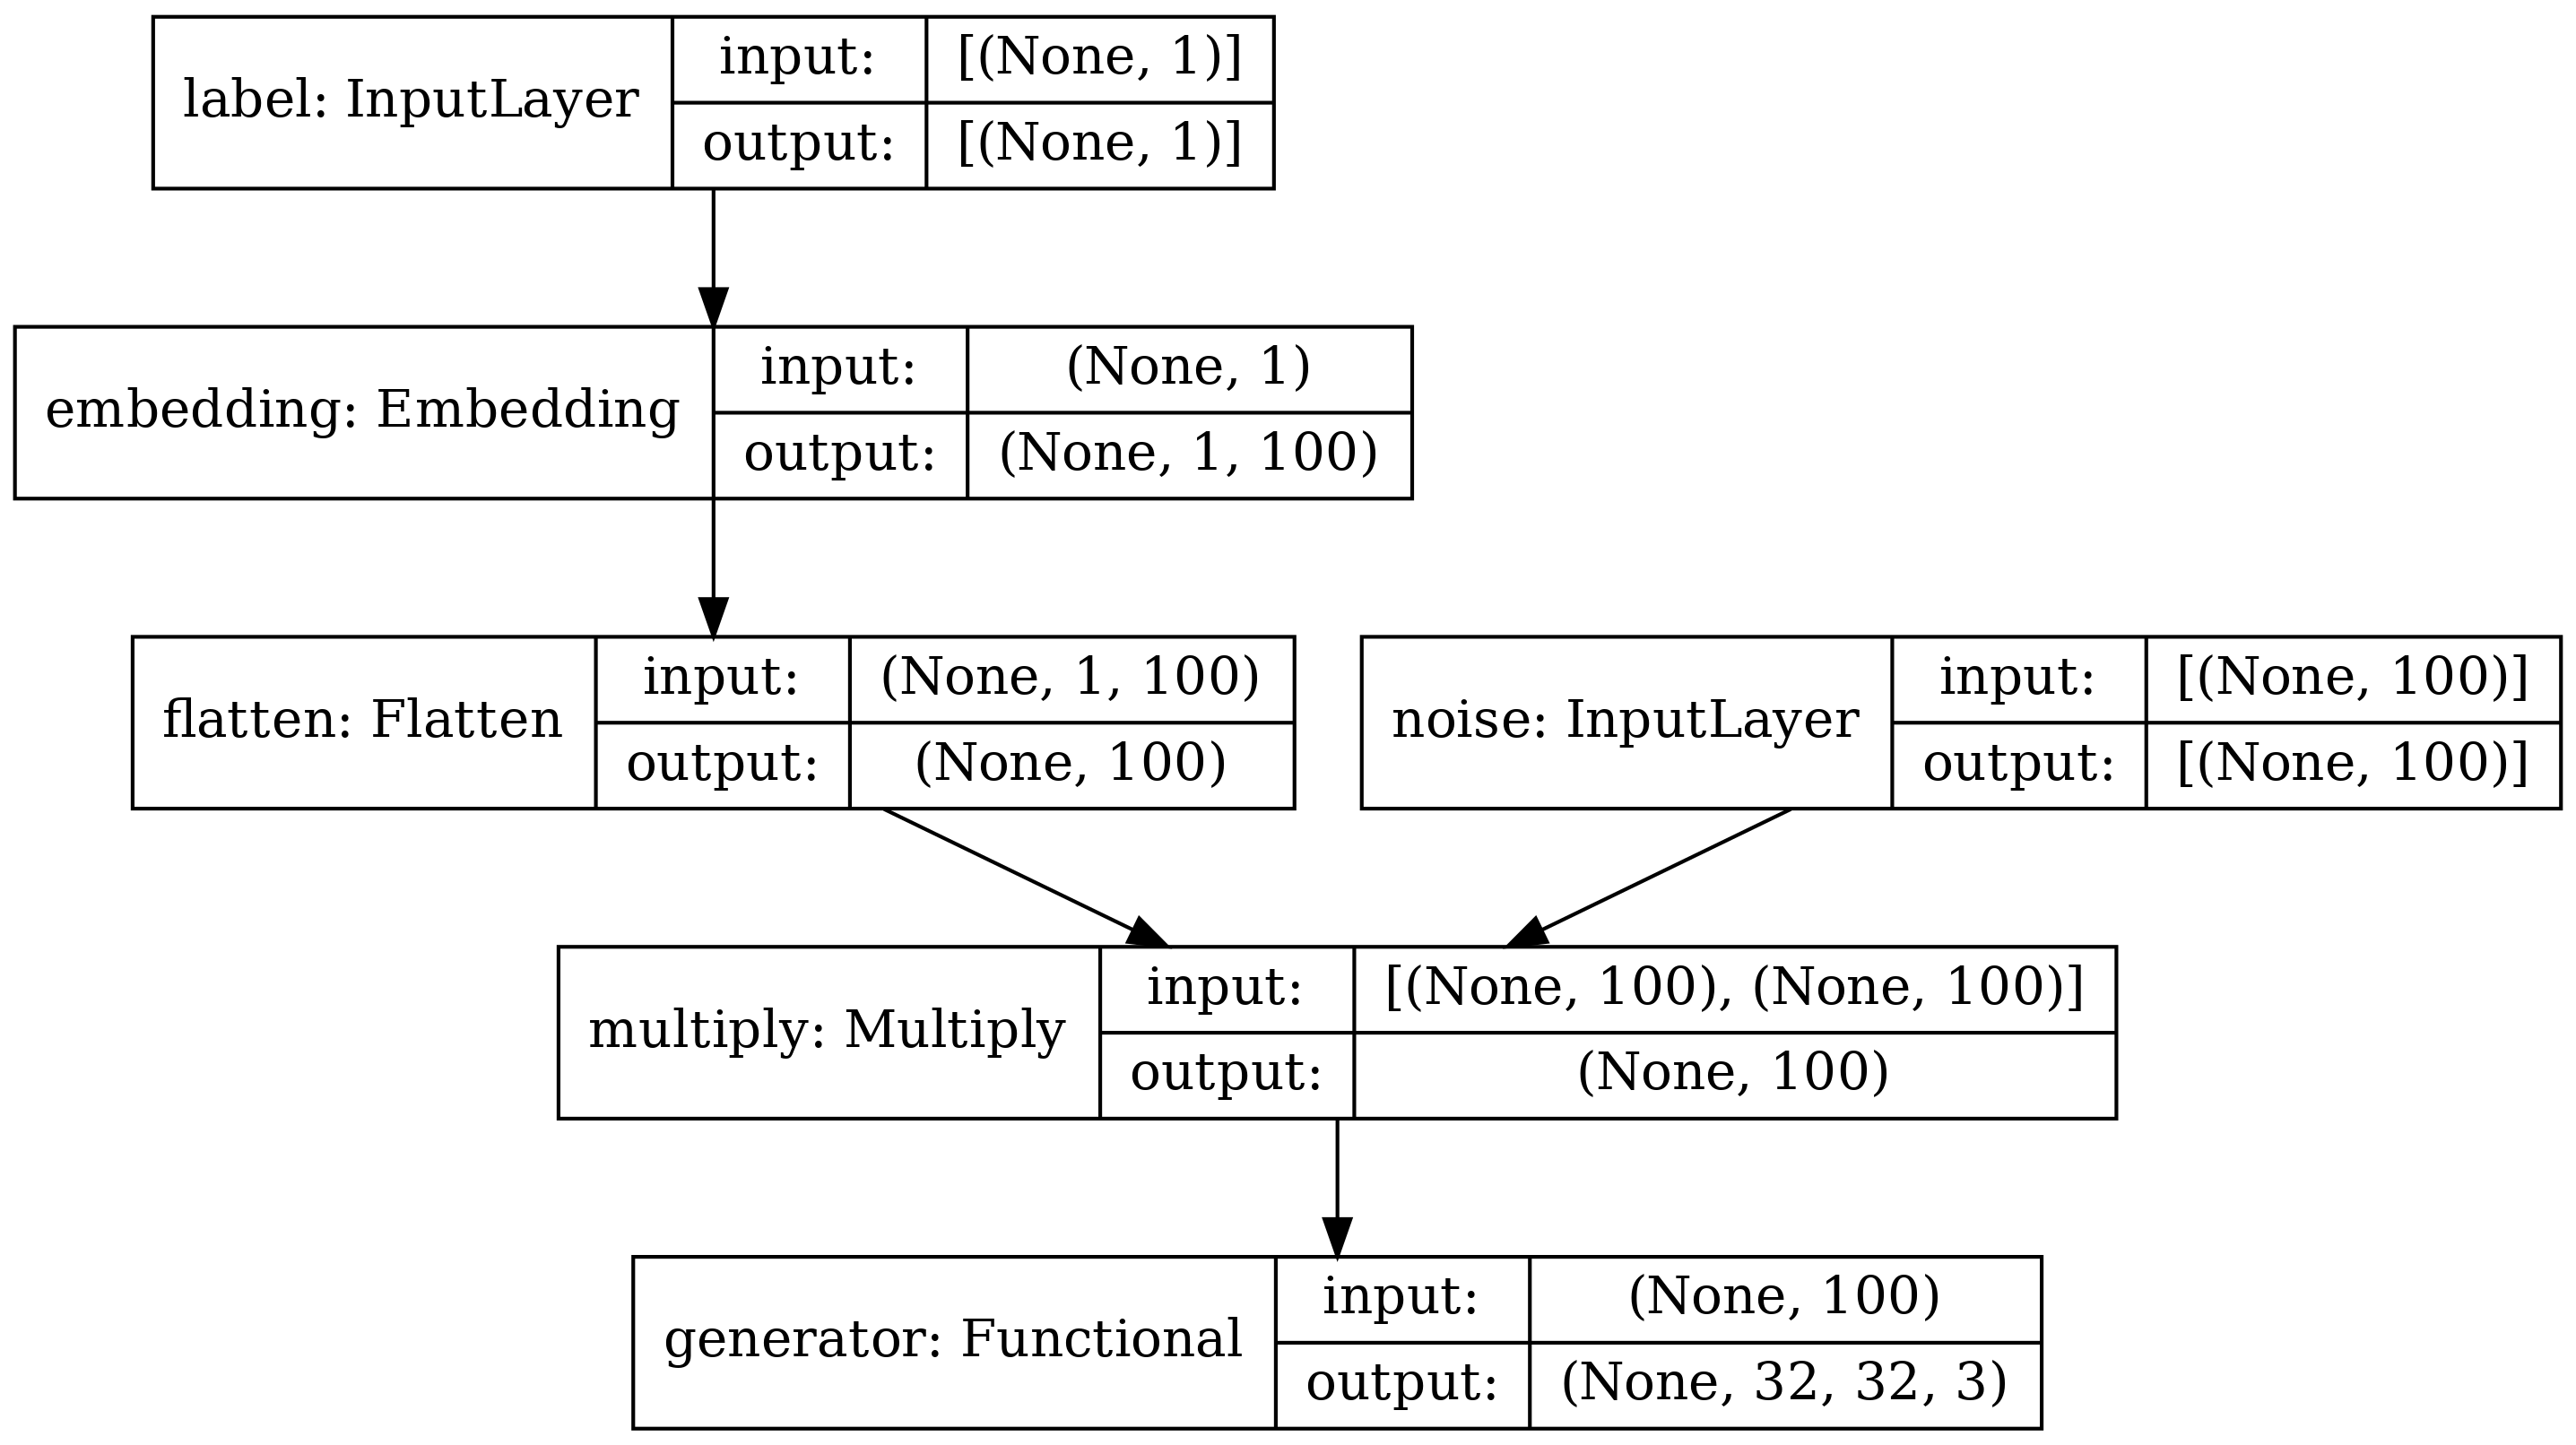
\includegraphics[width=10cm]{images/label_noise_embedding.png}
	\caption{A zajvektor és a címke összeállítása a generátor bemeneteként}
	\label{fig:labelnoiseembedding}
\end{figure}

A Diszkriminátorban a kondicionálást a modell belsejében hajtom végre. Mivel a Diszkriminátorunk a Generátor tükörképének is tekinthető, így a Diszkriminátor esetén nem a képpel együtt kerül be a címke a modellbe, hanem a modell által kinyert belső reprezentációkkal kerül összeszorzásra a címkét reprezentáló vektor, az utolsó teljesen összekapcsolt réteg előtt. A label conditioning technikát felvető cikkben megemlítették a \textit{dropout} réteg használatát is, így a teljesen összekapcsolt réteg előtt beillesztettem egy olyan réteget is.
A Diszkriminátor felépítése \aref{fig:labeldiscriminator}. ábrán figyelhető meg.

\begin{figure}[h]
	\centering
	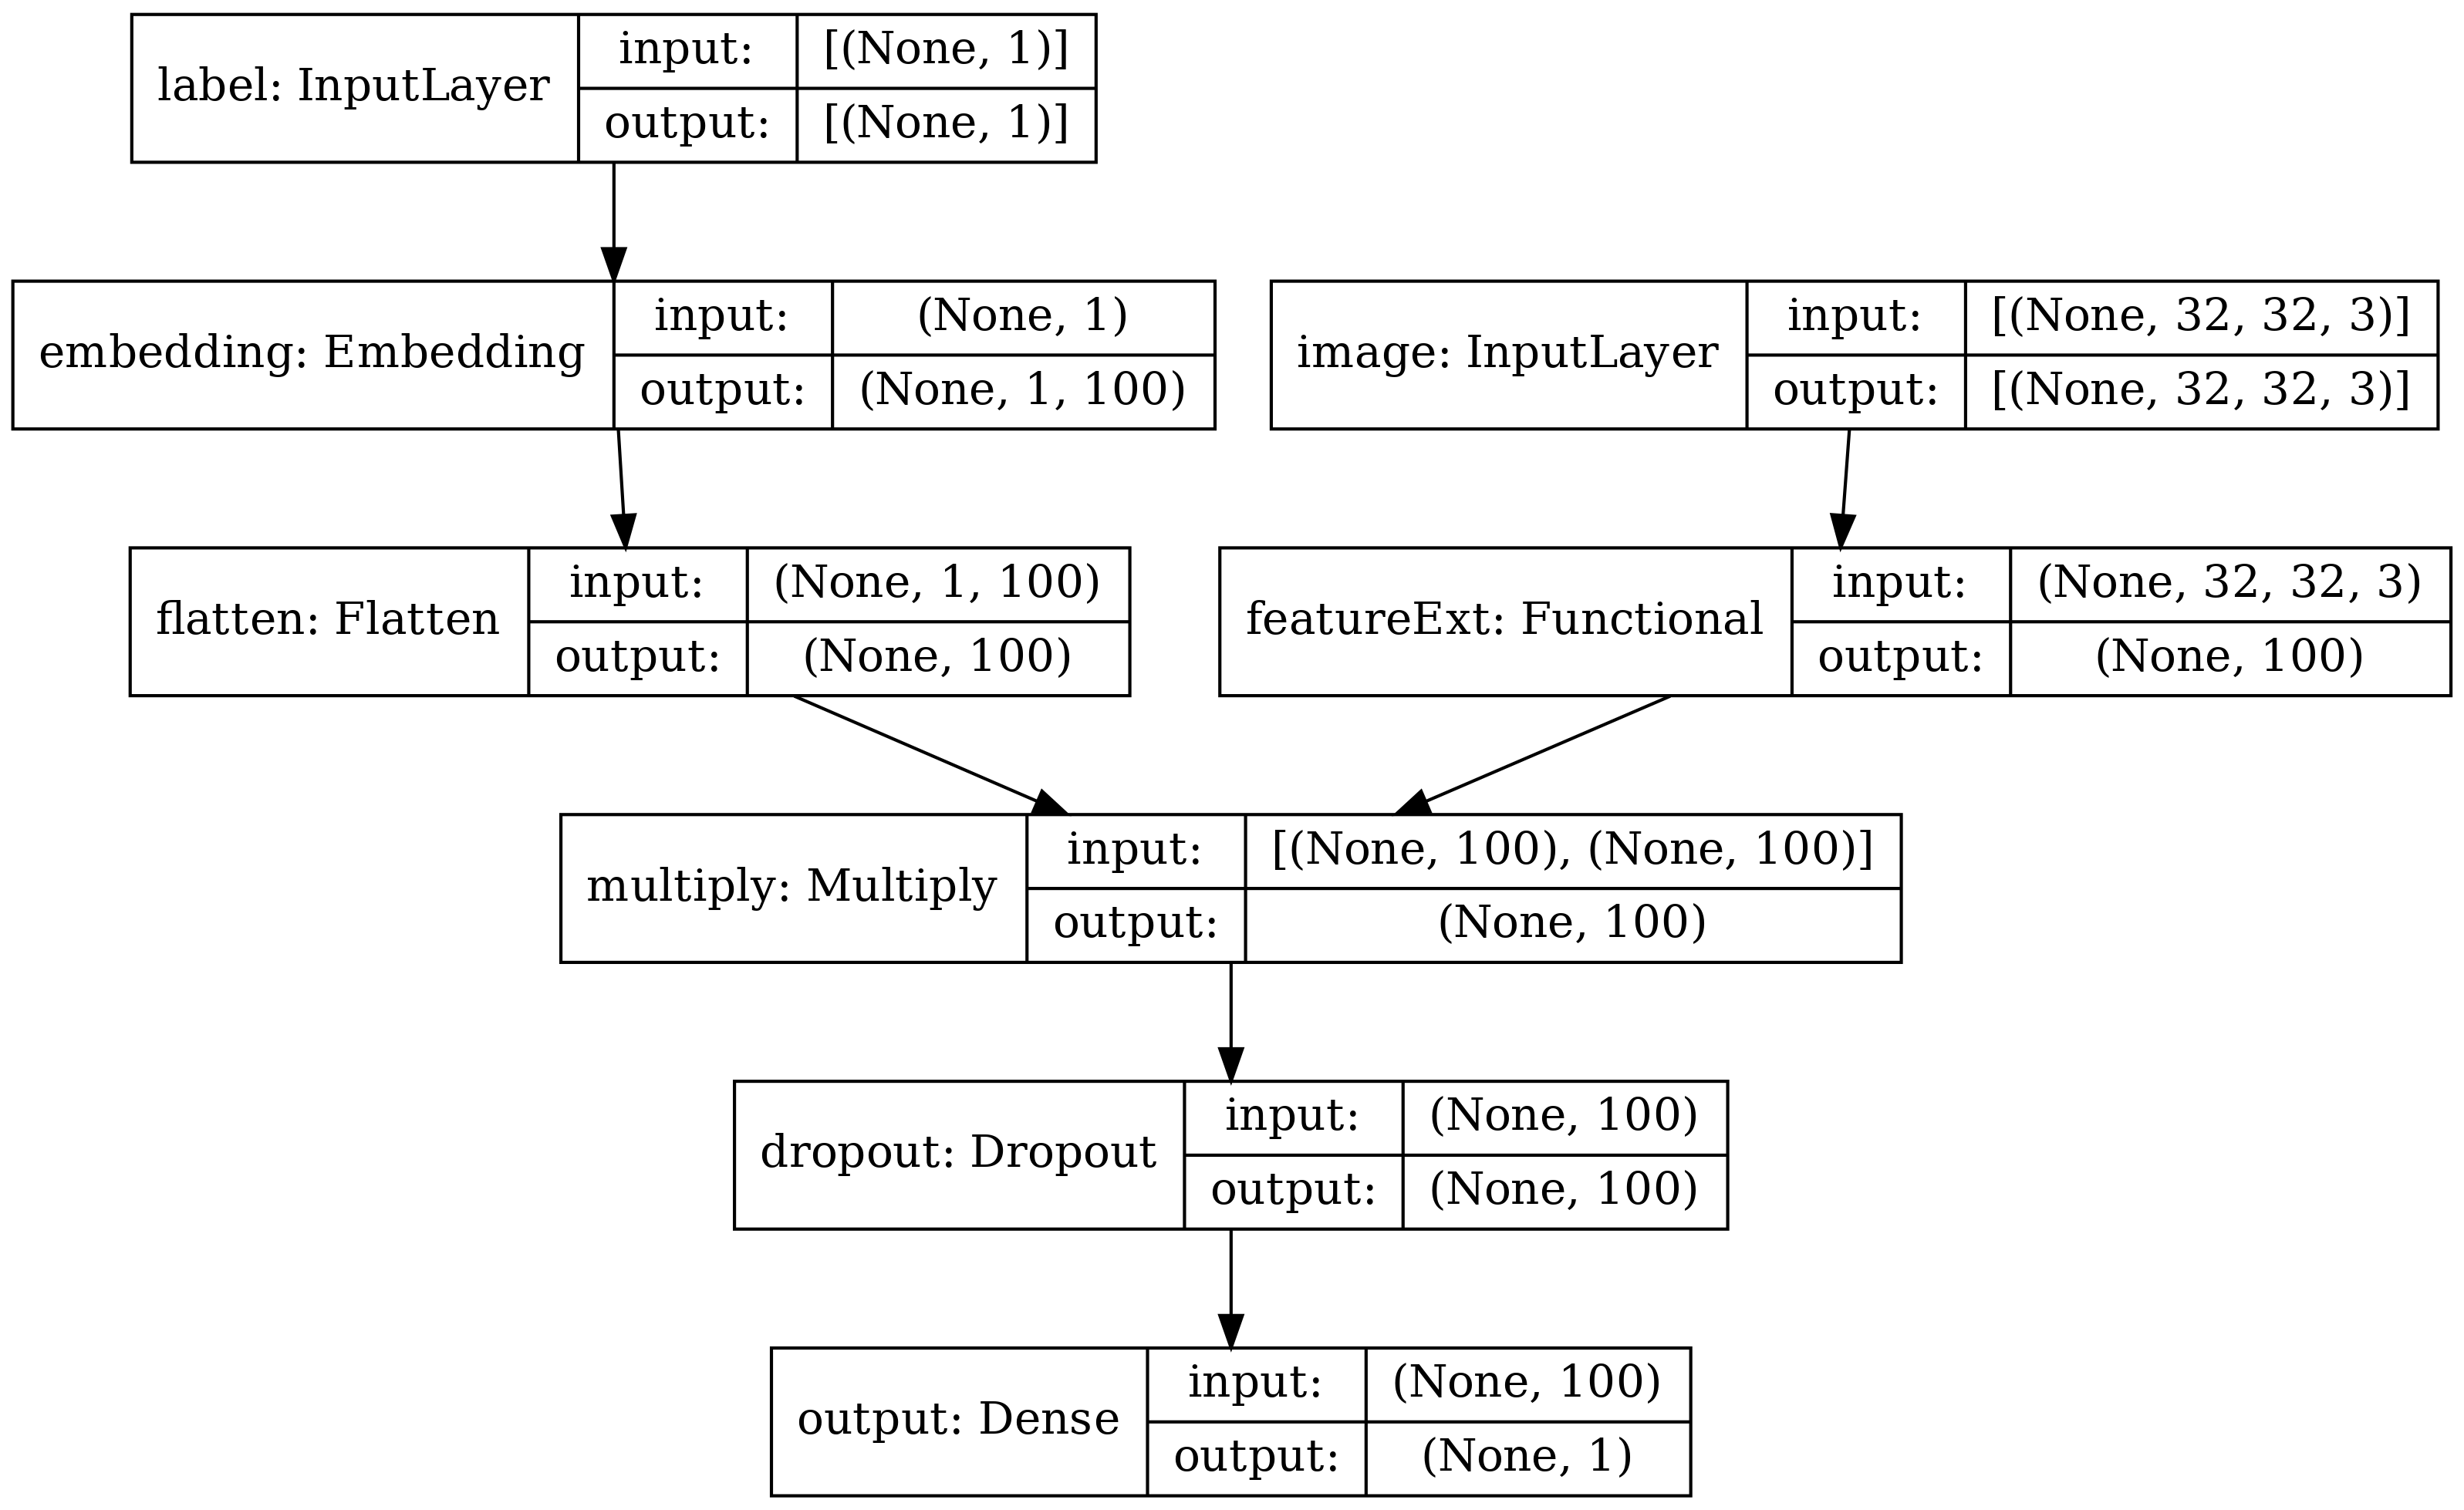
\includegraphics[width=10cm]{images/label_discriminator.png}
	\caption{A belső reprezentá és a címke összeállítása a diszkriminátorban}
	\label{fig:labeldiscriminator}
\end{figure}

A betanított háló kimeneteire példát \aref{fig:labelconditioning}. ábrán láthatunk, amely a már említett Cifar-10 adathalmaz 10 darab osztályára tanult be. A tanítás során megfigyeltem, hogy az osztályokon belül jelentkezik a mode-collapse jelensége, amely a regularizációs technikák alkalmazása mellett valamelyest javítható, viszont nem sikerült úgy betanítani a modellt, hogy igazán változatos képeket generáljon. A bemeneti zajvektor dimenziójának növelésével is némileg később jelentezett a mode-collapse, viszont egy ilyen kisebb példánál, $32 \times 32$-es felbontás mellett nem indokolt az 512 dimenziójú zajvektor használata, így ez nem tekinthető megoldásnak a mode-collapse-re, hiszen a modellek paramétereinek száma is megnövekedett a GAN-ban.
A technika másik hátránya, hogy az osztályok között igen éles határ alakul ki, vagyis nem lehet olyan bemeneti címkét megadni, aminek hatására kevert osztályokat is ki tudna generálni a modell. Minden esetben csupán egyetlen osztály képének megalkotására képes, még akkor is, ha nem egész értékeket adunk meg címkének. Két címke között interpolálva egyszerűen az egyik határponton átugrik a modell kimenete a következő címkének a kimenetére.

A tanítás kiegyensúlyozatlansága, és a kevert osztályok reprezentálásának hiánya miatt úgy gondoltam, hogy nem ezen megoldás lesz számomra a legkedvezőbb.

\begin{figure}[h]
	\centering
	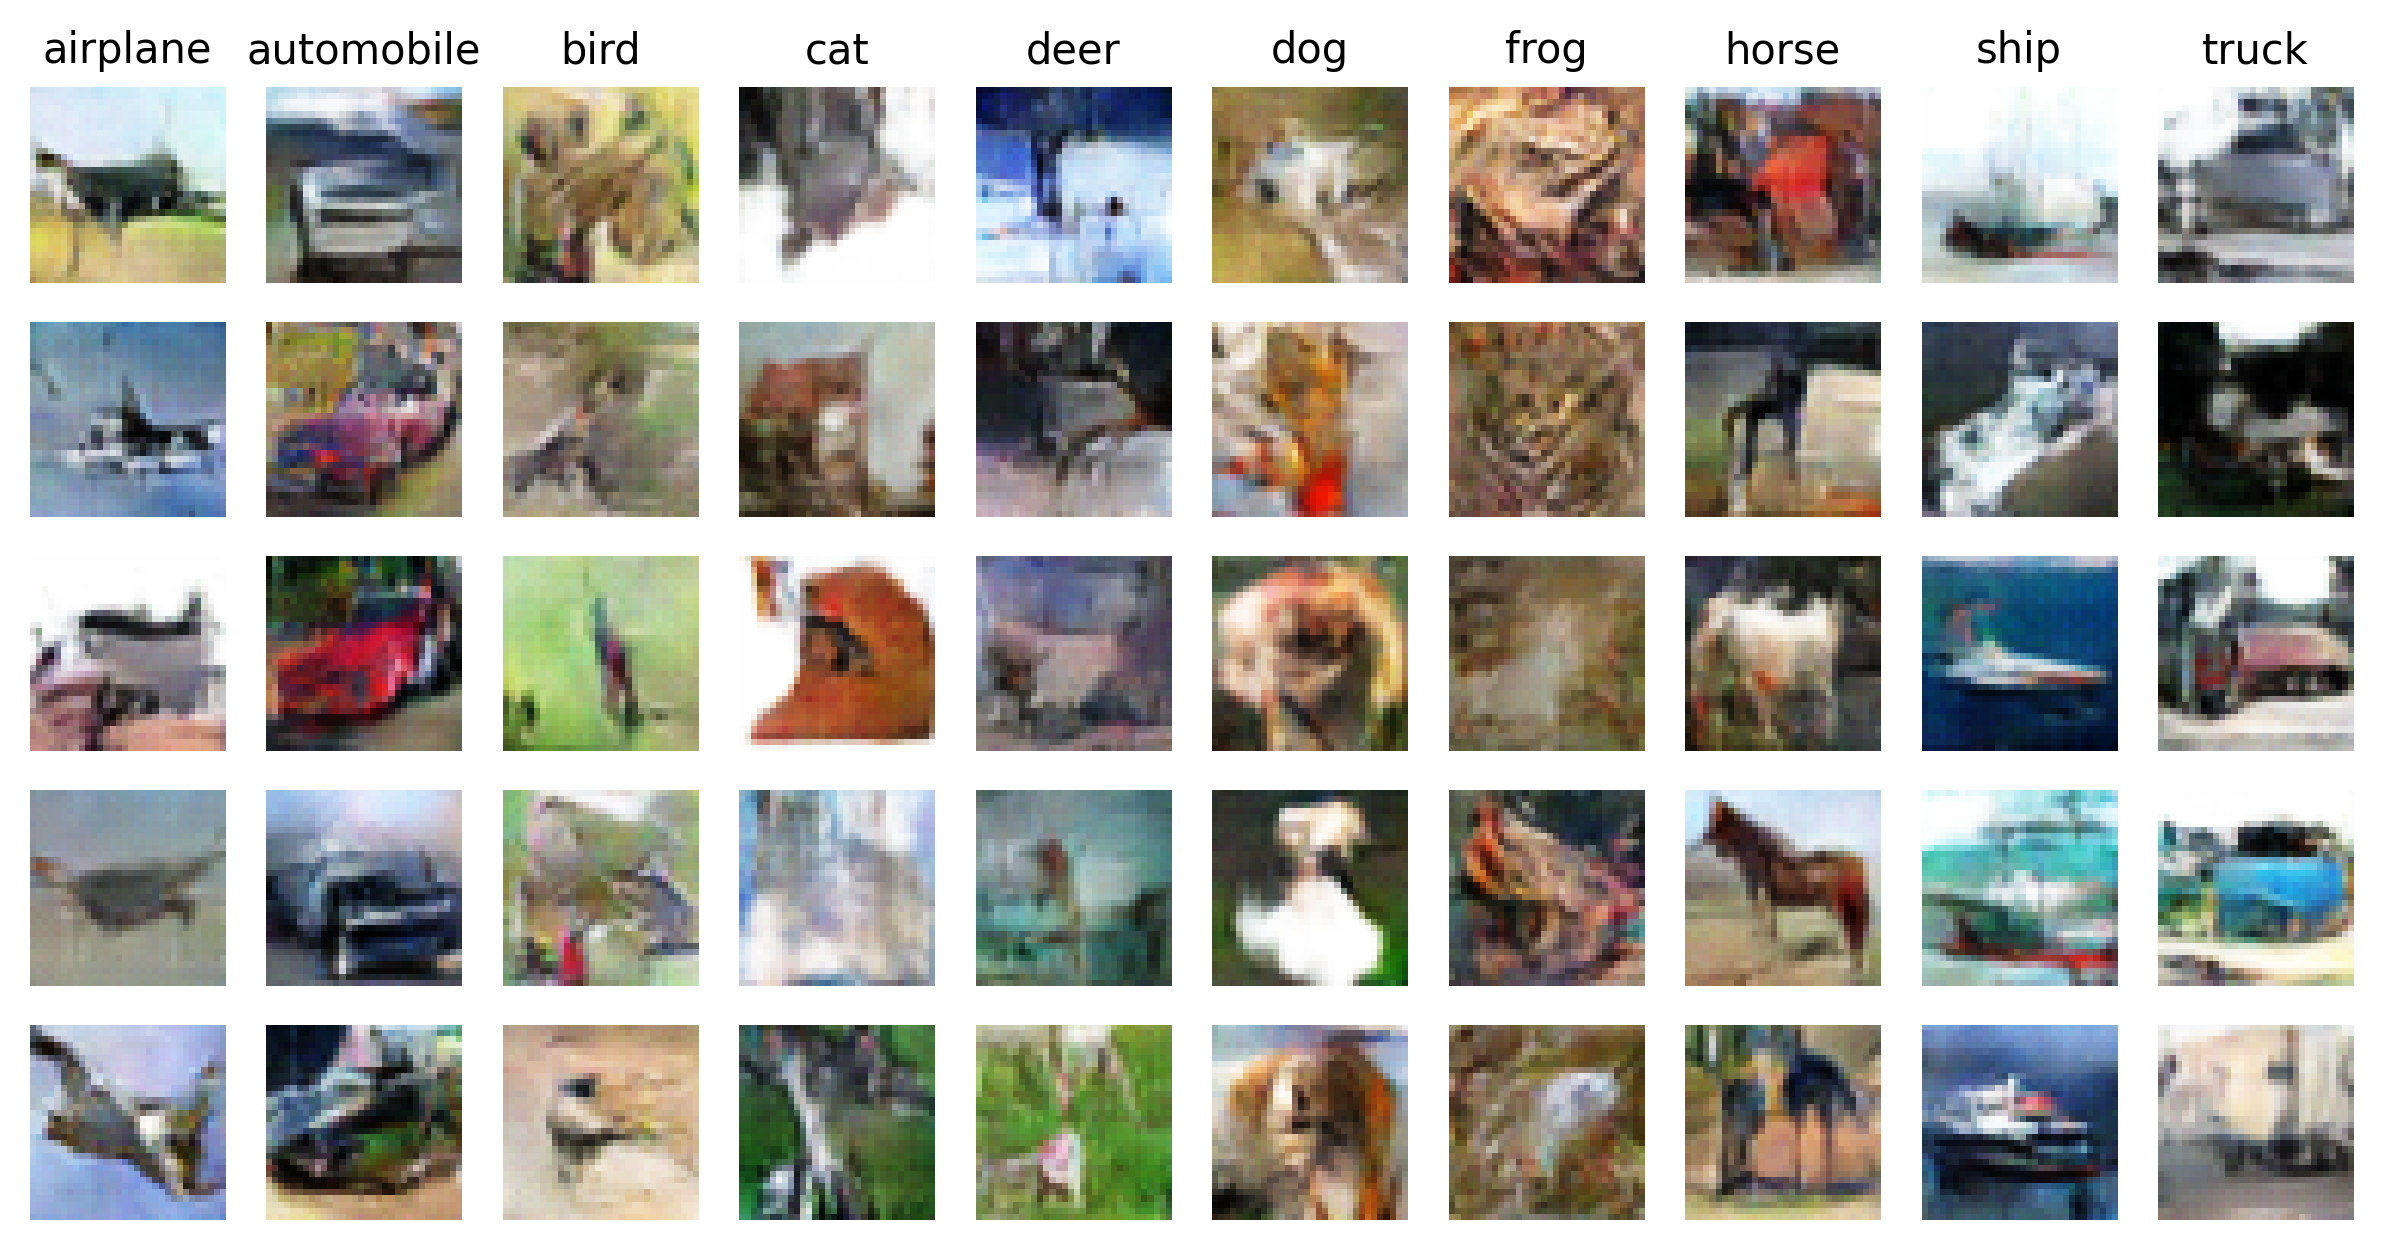
\includegraphics[width=13cm]{images/label_conditioning.png}
	\caption{Label conditioning technikával tanított Generátor kimenetei}
	\label{fig:labelconditioning}
\end{figure}

\SubSection{Multi-Scale Gradient architektúra}

Egy másik kiegészítésként a \textit{Multi-Scale Gradient} (MSG) alapján több ki- és bemenettel láttam el a Generátort és a Diszkriminátort \cite{karnewar2020msg}. Igyekeztem az eredeti modellemet kiegészíteni és alkalmazni az MSG-ben látottakat, vagyis az U-net szerű kapcsolatokat. Ugyan a \textit{Multi-Scale Gradient} architektúra implementálása nem hozta el az architektúrához publikált eredményeket, viszont a kigenerált képek minőségét valamelyest javította. Az eredeti és ezen modell eredményeinek összehasonlítására az alfejezet végén láthatunk majd összehasonlítást.

A kibővített modell Generátora összességében megegyezik az eredeti modellel, csupán több kimenettel rendelkezik. A belső rétegekben található reprezentációkból egy-egy konvolúciós réteg segítségével állítja elő a modell a kimeneteket. A korábban említett \textit{toRGB} rétegnek felelnek meg ezek a rétegek. Az aktivációs függvénye ezen rétegeknek a tangens hiperbolikusz, hasonlóan az eredeti modell utolsó rétegéhez.
A Generátorba került még minden dekonvolúciós réteg után egy-egy \textit{BatchNormalization} réteg is, továbbá alkalmazásra került a He-féle inicializálási stratégia is.
A saját implementációmban a \textit{toRGB} konvolúciós réteg a következő táblázatban megfigyelhető paraméterekkel lett ellátva:

\small{
\begin{center}
\begin{tabular}{@{\extracolsep{6pt}} c c c c c }
	\hline
	\multicolumn{5}{l}{\textbf{\textit{toRGB} konvolúciós réteg}} \\
	\hline
	Filterek száma & Kernelméret & Strides & Padding & Aktivációs függvény\\
	\cline{1-1} \cline{2-2} \cline{3-3} \cline{4-4} \cline{5-5}
	3 db & $4 \times 4$ & $1 \times 1$ & "same" & tangens hiperbolikusz\\
	\hline
\end{tabular}
\end{center}
}

A 4 darab \textit{toRGB} réteg további 46092 darab hiper-paramétert jelent, amelyek a tanítás során kerülnek finomhangolásra. Az eredeti modell milliós hiper-paraméter nagysága mellett nem tűnik olyan nagy kiegészítésnek. Viszont ezen rétegeknek is meg kell tanulnia a belső reprezentációk megfelelő leképzését a három színcsatornára.

\Aref{fig:msgGenerator}. ábrán egy olyan Generátor figyelhető meg, amely 4 kimenettel rendelkezik és rendre: $4 \times 4$, $8 \times 8$, $16 \times 16$ és $32 \times 32$ felbontású képeket generál egyszerre. A kép nagysága miatt csupán $32 \times 32$ maximális felbontásig felépített modell került ábrázolásra.

\begin{figure}[h]
	\centering
	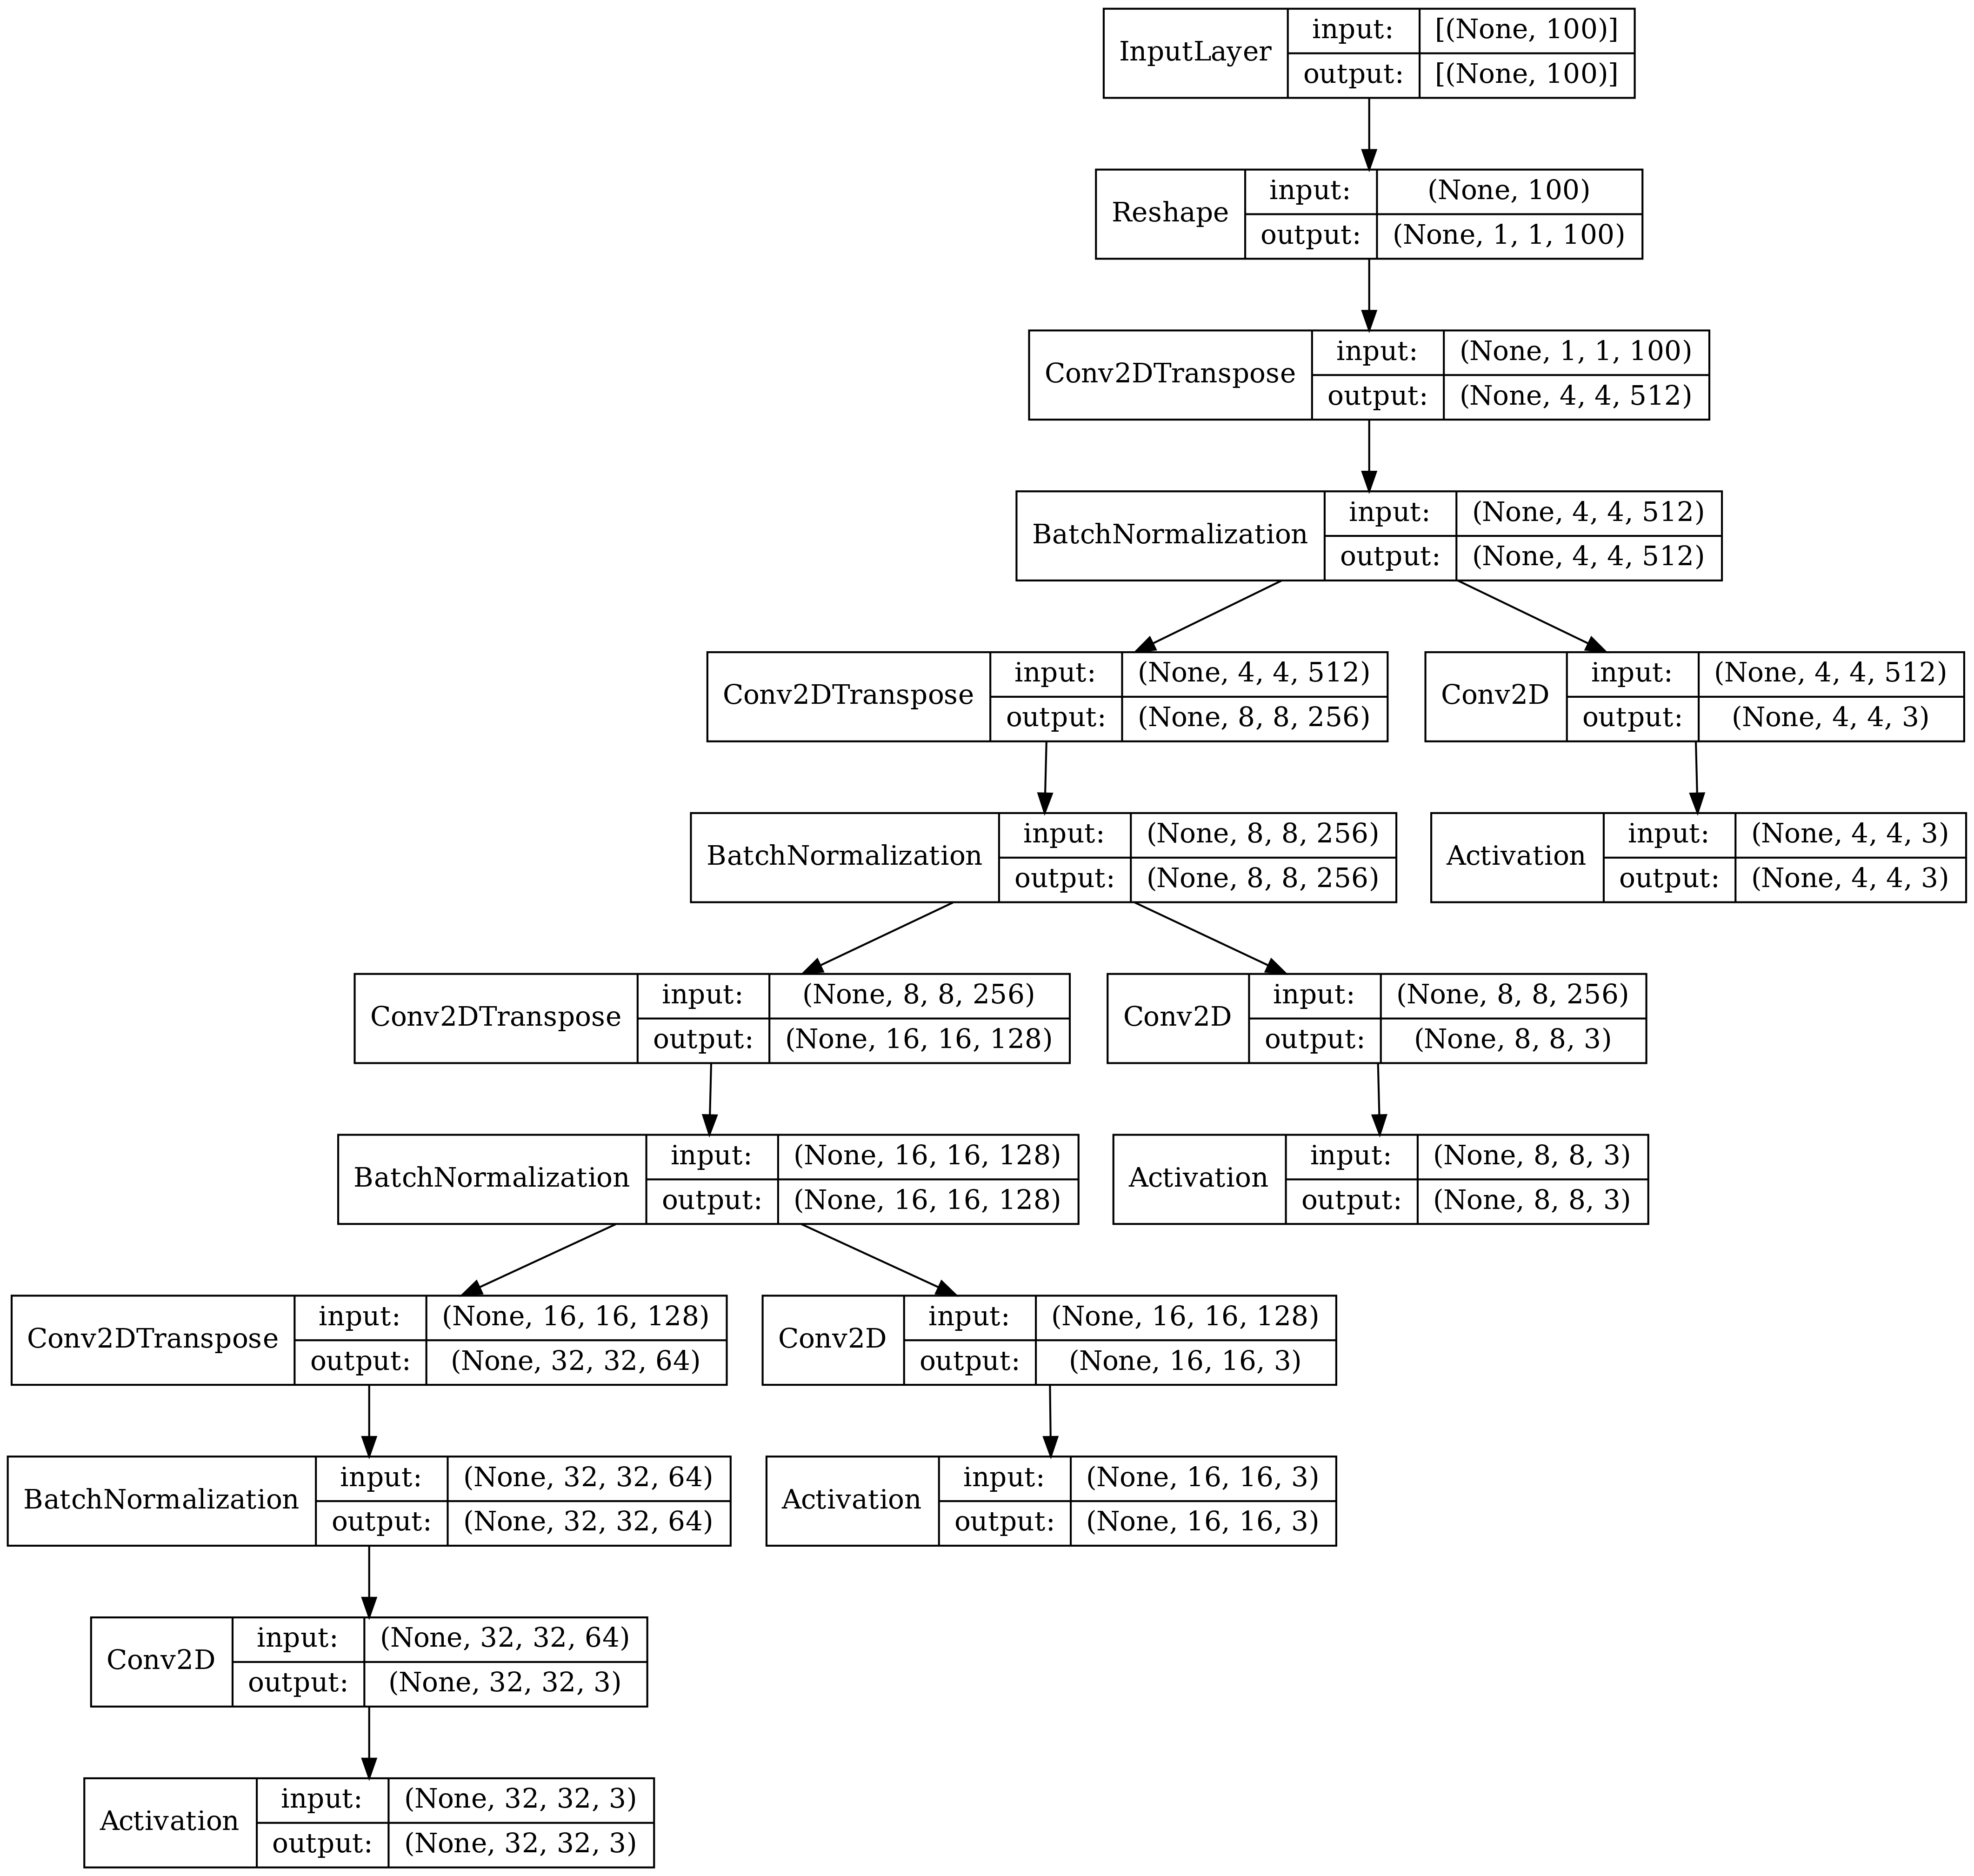
\includegraphics[width=15cm]{images/msgGenerator.png}
	\caption{Generátor több kimenettel, $32 \times 32$ maximális felbontással}
	\label{fig:msgGenerator}
\end{figure}

A Diszkriminátor modell architektúrája további módosításokat igényel. A bemeneteinek száma meg fog egyezni a Generátor kimeneteinek számával, a kapott képeket pedig a megfelelő helyre, a belső reprezentációihoz fűzi hozzá. A bemenetekből \textit{fromRGB} réteggel nyeri ki a feature-öket az összefűzéshez. Ezen konvolúciós rétegek feladata, hogy a három színcsatornával rendelkező képeket olyan reprezentációvá alakítsa át, amely az adott szint csatornaszámával megegyező csatornákat tartalmaz. Ezt úgy éri el, hogy a filterek számát a kívánt csatornaszámra állítjuk és "same" padding-et alkalmazunk $ 1 \times 1 $ stride értékek mellett. A kernelméret jelen esetben $ 3 \times 3 $-as, mivel ezen új rétegek a megnövekedett filterszámokkal igen sok további hiperparamétert adnak az eredeti modellhez.
Az egyértelműség érdekében a \textit{fromRGB} rétegek paraméterei a következő táblázatban is összefoglalásra került:

\small{
	\begin{center}
		\begin{tabular}{@{\extracolsep{6pt}} c c c c c }
			\hline
			\multicolumn{5}{l}{\textbf{\textit{fromRGB} konvolúciós réteg}} \\
			\hline
			Filterek száma & Kernelméret & Strides & Padding & Aktivációs függvény\\
			\cline{1-1} \cline{2-2} \cline{3-3} \cline{4-4} \cline{5-5}
			Az adott szinttel megegyező & $3 \times 3$ & $1 \times 1$ & "same" & nincsen\\
			\hline
		\end{tabular}
	\end{center}
}

\begin{figure}[h]
	\centering
	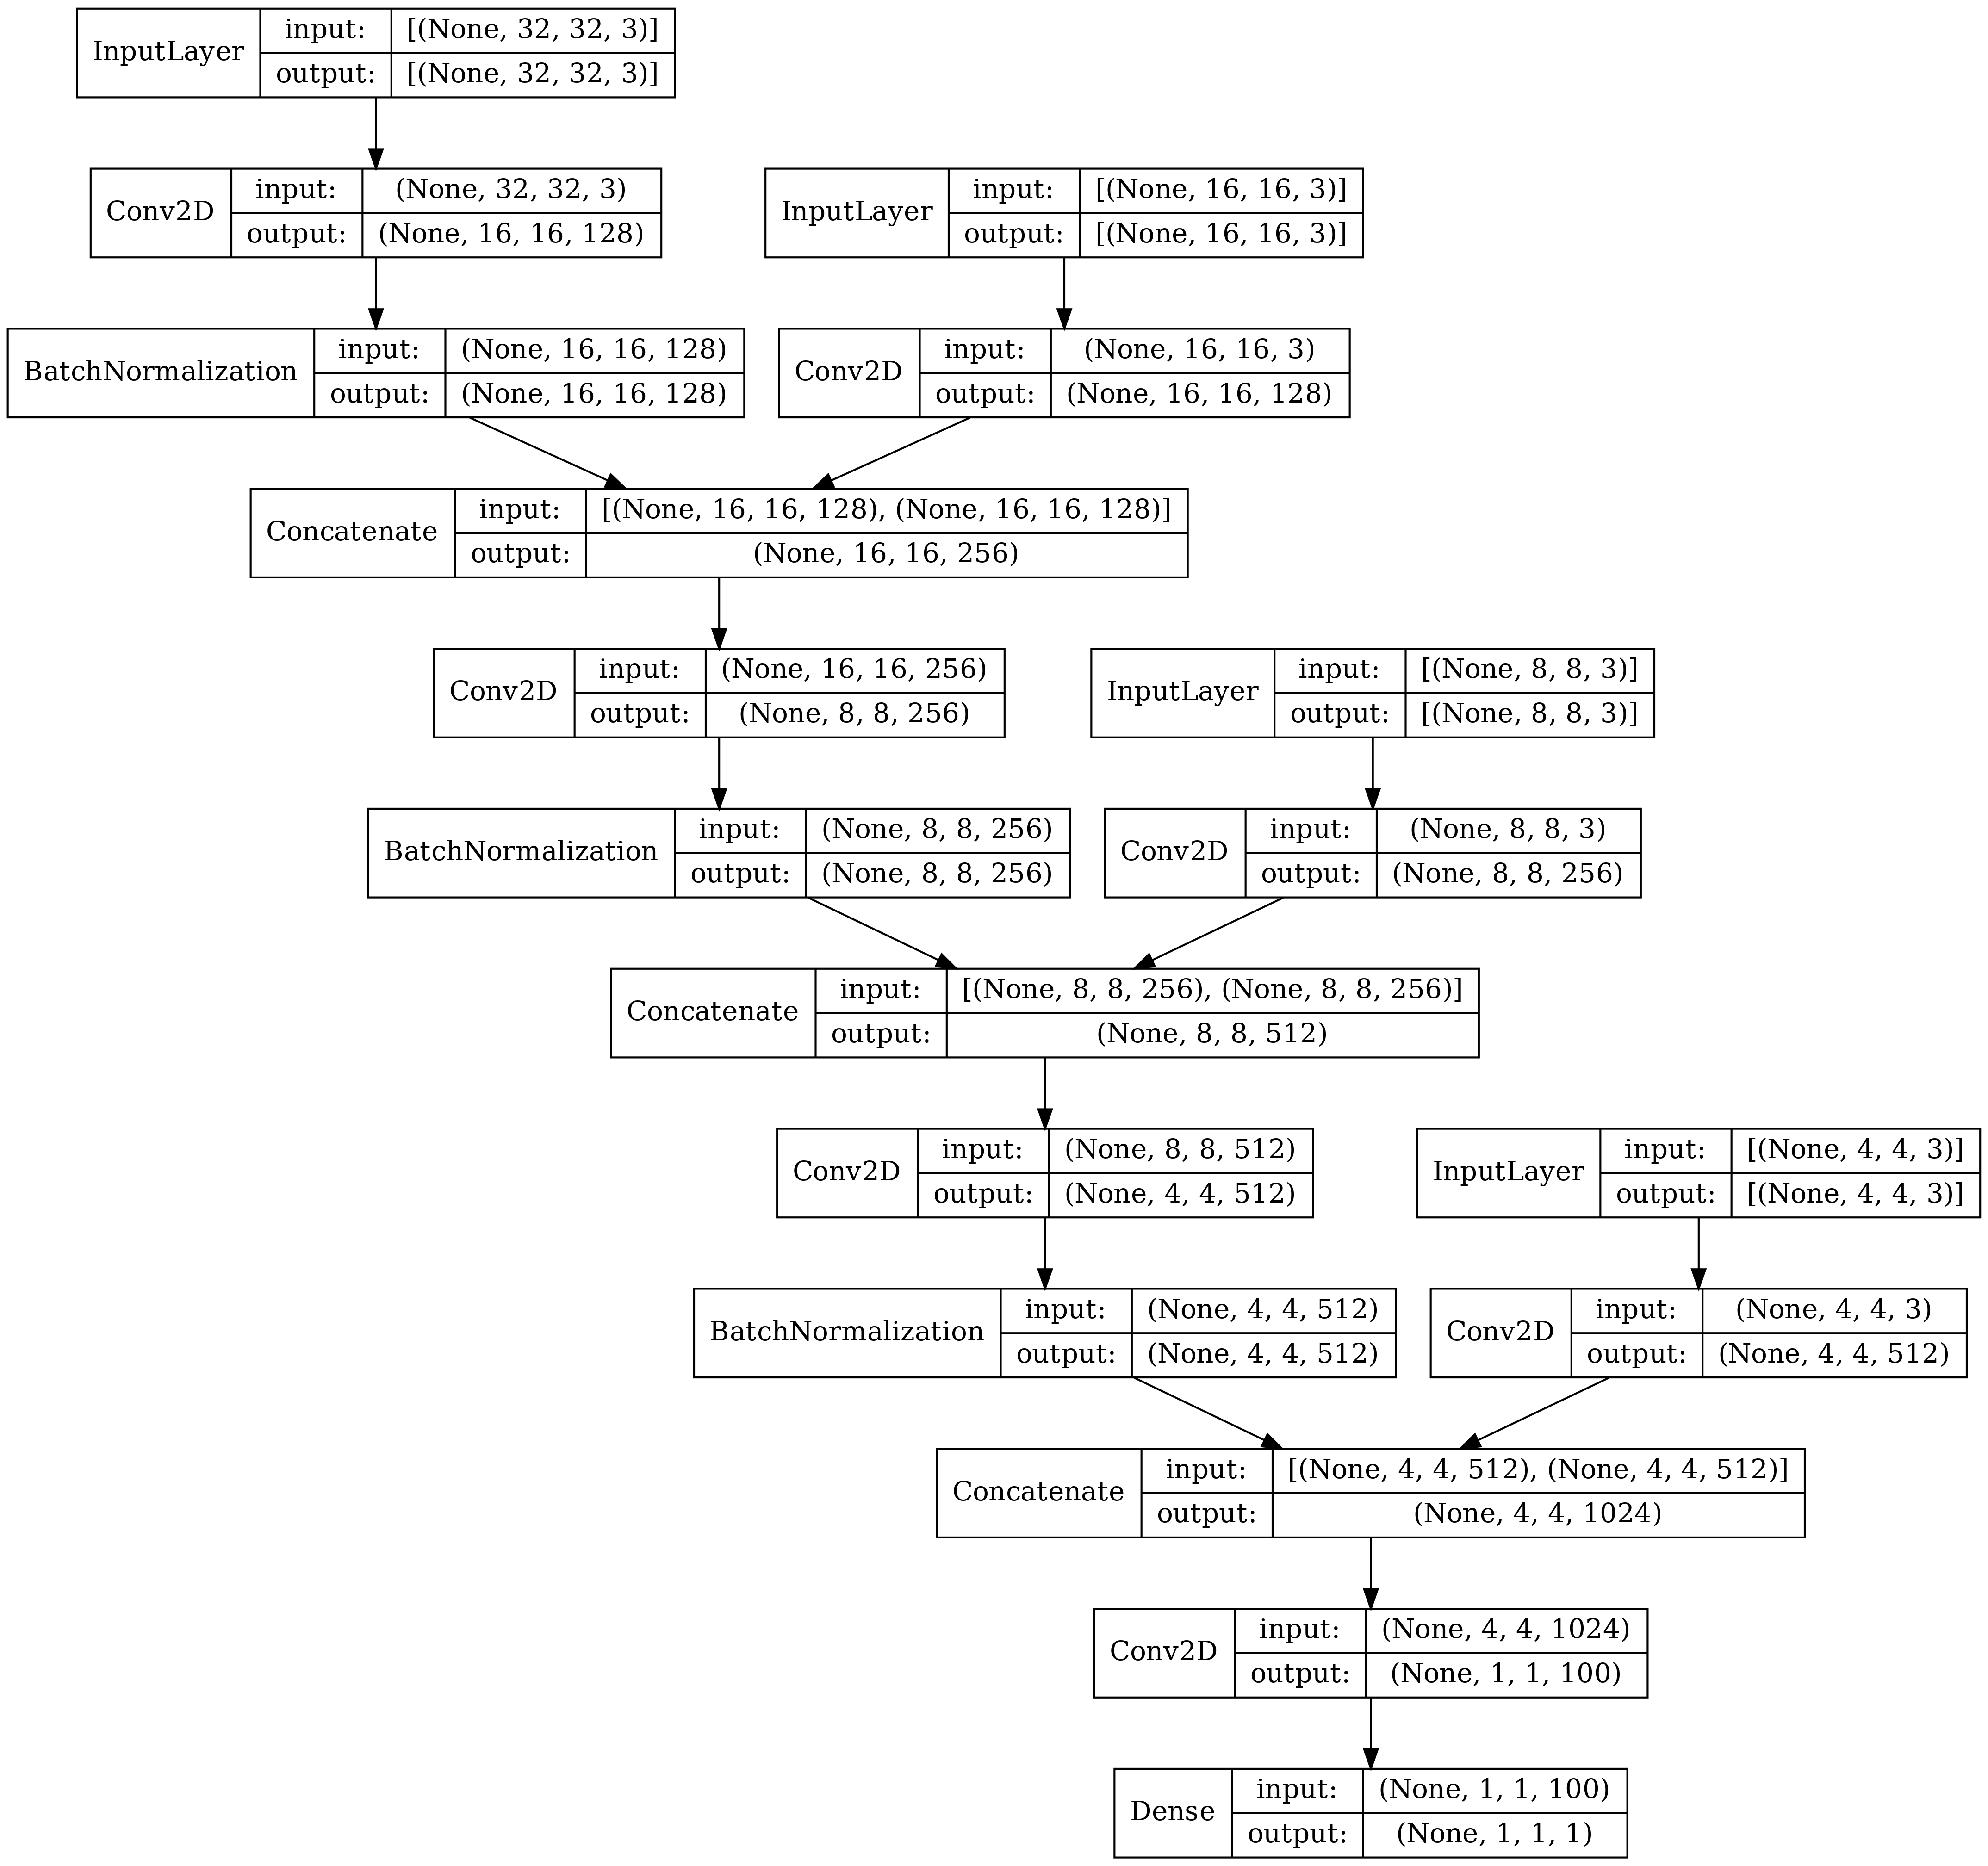
\includegraphics[width=15cm]{images/msgDiscriminator.png}
	\caption{Diszkriminátor több kimenettel $32 \times 32$ maximális felbontással}
	\label{fig:msgDiscriminator}
\end{figure}

A Diszkriminátor is megőrizte az eredeti felépítését (\ref{fig:msgDiscriminator}. ábra), viszont a \textit{fromRGB} rétegek igen sok további hiper-paramétert adnak hozzá a modellhez. Itt már milliós nagyságrendű új paraméter kerül a modellbe, és ezen kiegészítés hatására az eredetileg 3,5 millió paraméterrel rendelkező modell máris 7,1 millió paraméterrel rendelkezik. Így nem érvényesül a korábban felállított tükörkép-szerkezet, vagyis amikor a Diszkriminátor a Generátor fordítottja. A \textit{fromRGB} rétegek filtereinek számának hatására nő meg a paraméterek száma ilyen nagy mértékben. A módszert bemutató cikkben többféle módon is vizsgálták a bemenet összefűzés előtti feldolgozását. A nyers bemeneti képeken nem alkalmaztak végül transzformációt, és a cikkben felvázolt architektúrához az nyújtotta a legjobb megoldást. A saját implementációmat is ilyen módon készítettem el kezdetben. Viszont azt figyeltem meg, hogy csupán a nyers képek hozzáfűzése mellett a modell először a legnagyobb felbontású képeket tanulja meg megfelelően kigenerálni és a tanítás során igen lassan kerülnek a súlyok olyan állapotban, hogy az alsóbb rétegek is megfelelően megtanulják a kimenet elkészítését. A legkisebb felbontású kimeneten látszólag nem is tanult a modell, csupán random zaj jelent meg. Az architektúrámra alkalmazva a \textit{fromRGB} rétegeket megoldotta a legalsó rétegek tanulási problémáját.

\begin{figure}[h]
	\centering
	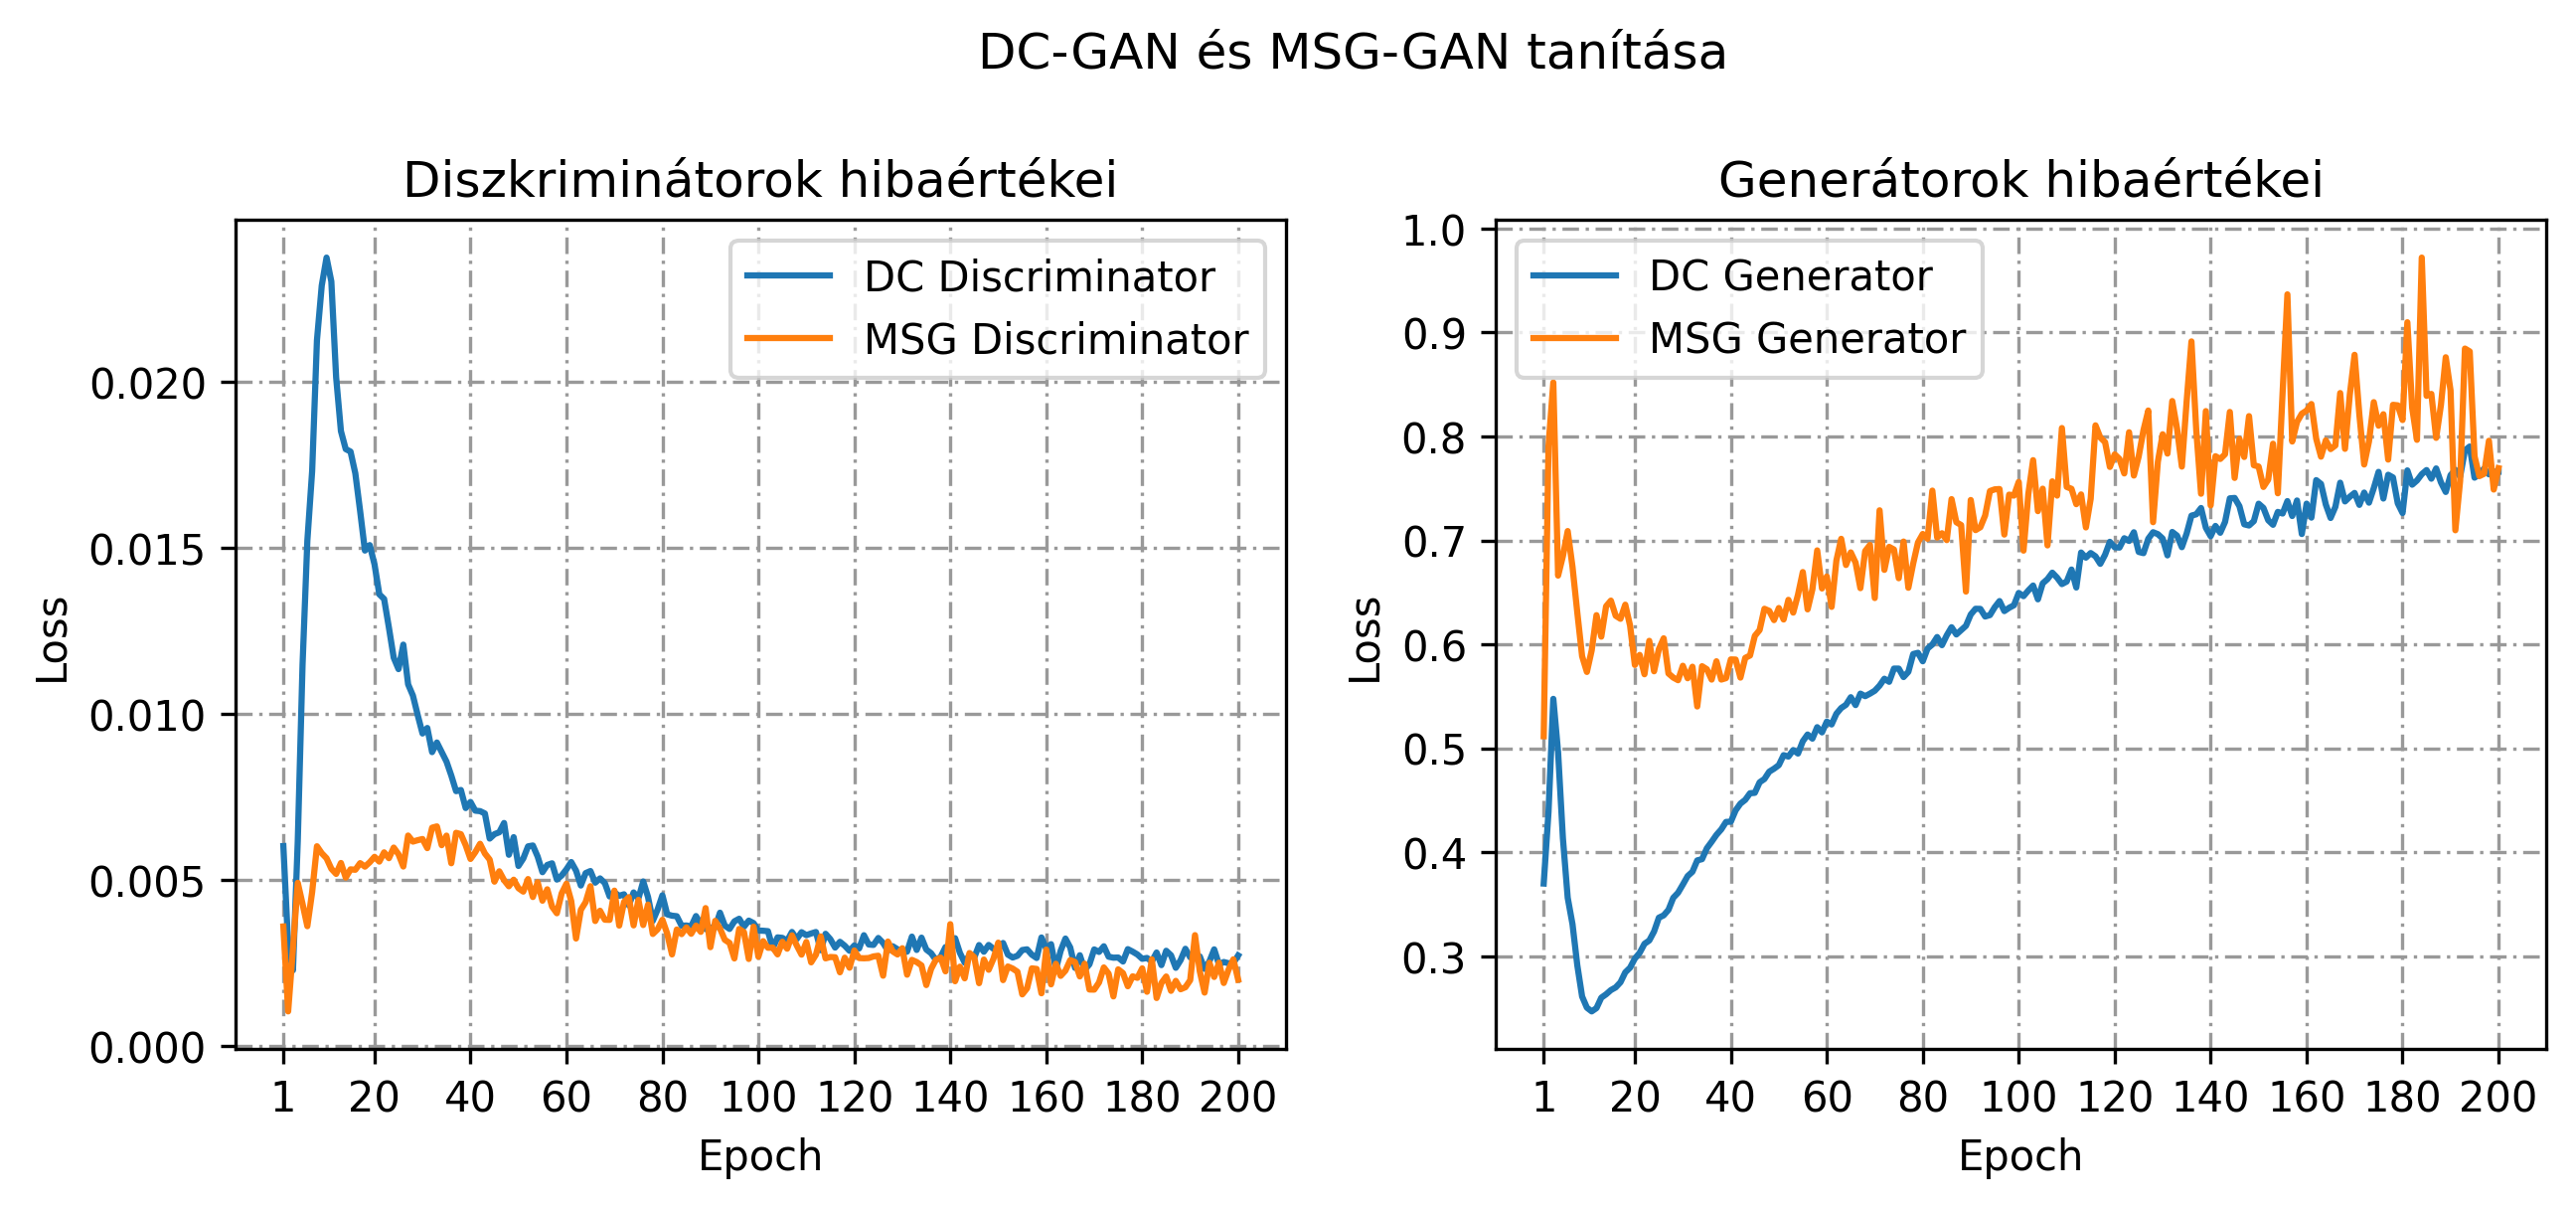
\includegraphics[width=15cm]{images/dc_vs_msg.png}
	\caption{A mély konvolúciós GAN és az MSG GAN tanítása során mért hibaértékek az AFHQ adathalmazon tanítva}
	\label{fig:dcvsmsg}
\end{figure}

\Aref{fig:dcvsmsg}. ábrán megfigyelhetők az eredeti és a kibővített modell Generátorainak és Diszkriminátorainak hibafüggvényei. Narancssárga színnel figyelhetjük meg az újonnan bemutatott modell hibaértékeit a tanulás alatt. A tanítás előrehaladtával hajlamosabb az oszcillációra a modell, viszont ami az ábrán még megfigyelhető, hogy a hibák értéktartománya sokkal szűkebb a Diszkriminátor és a Generátor esetében is.

\begin{figure}[h]
	\centering
	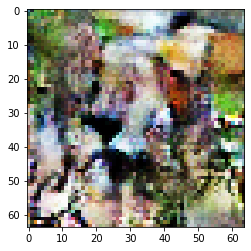
\includegraphics[width=5cm]{images/collapsed_mode.png}
	\caption{Egy "összeomlott-mode" a generátorban}
	\label{fig:collapsed_mode}
\end{figure}

Ezen kibővítés sem tökéletes. Az egyik, AFHQ adathalmazon betanított modell esetében a képek generálása során felfigyeltem egy visszatérő képre, amelyen érdekes mintázatok jelentek meg, viszont nem hasonlít az adathalmaz egyik elemére sem. A jelenségre, a mode-collapse fejezetben is említett, \textit{lokális mode} vagy \textit{összeomlott-mode}-ként is hivatkozhatunk. A látens tér bizonyos tartományában mintavételezett pontokra ugyanazt a képet generálja ki a modell, viszont a további pontokat nézve nem figyelhető meg semmiféle ismétlődő mintázat vagy egyéb mode-collapse-re utaló anomália. \Aref{fig:collapsed_mode}. ábrán látható egy példa az összeomlott-mode-ra. 

\Aref{fig:msg_output}. ábrán a Generátor kimeneteit figyelhetjük meg $4 \times 4$-es felbontástól egészen a $64 \times 64$ felbontásokig. Ezen ábrára tekintve érthető meg igazán a technika mögötti gondolat: a globális összefüggőségek az alacsonyabb felbontások mellett betanult jellegzetességek hatására alakul ki. A magasabb felbontásokon pedig az egyes képrészek részletességeinek növelése történik.

\begin{figure}[h]
	\centering
	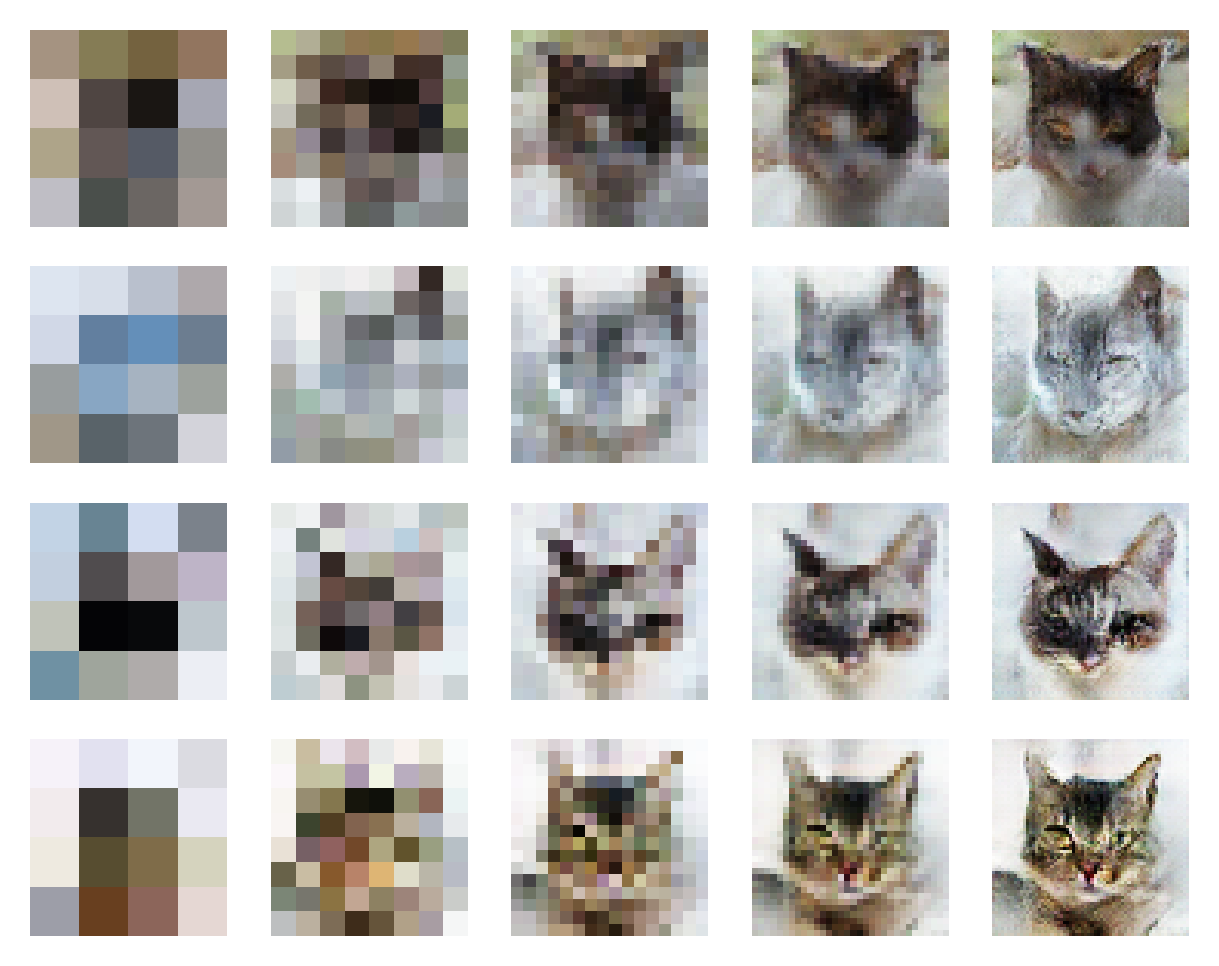
\includegraphics[width=12cm]{images/msg_output.png}
	\caption{Példa a Generátor kimeneteire $64 \times 64$ maximális felbontás mellett}
	\label{fig:msg_output}
\end{figure}

Az eredeti és ezen új modell teljesítményének méréséhez az Inception Score és a Fréchet Inception Distance metrikákat alkalmaztam. A méréshez a Cifar10 és az AFHQ adathalmaz elemein tanult mély konvolúciós (DC-GAN) és Multi Scale Gradient (MSG-GAN) generátorait használtam fel. A méréshez egységesen 10000 mintát generáltam mind a négy modellhez a tanításhoz is használt normális eloszlásból kapott látens vektorokkal. A mérés eredménye az alábbi táblázatban figyelhető meg.

%TODO FID mérés!
\begin{center}
	\begin{tabular}{@{\extracolsep{6pt}} l c c c c }
		\hline
		& \multicolumn{2}{c}{\textbf{IS}} & \multicolumn{2}{c}{\textbf{FID}}\\
		\cline{2-3} \cline{4-5}
		& Cifar10 & AFHQ & Cifar10 & AFHQ\\
		\hline
		DC-GAN & $5.4394 \pm 0.276$ & $4.9611 \pm 0.1464$ & $11.3$ & $11.3$\\
		MSG-GAN & $5.9588 \pm 0.1273$ & $6.0283 \pm 0.2169$ & $9.2$ & $9.2$\\
		\hline
	\end{tabular}
\end{center}

%dcgan cifar10
%(5.439416, 0.20759696)

%msggan cifar10
%(5.9587755, 0.12729427)

%dcgan afhq
%(4.9610844, 0.1464256)

%msggan afhq
%(6.0283036, 0.21691017)

\noindent Az IS esetében a magasabb érték jelent jobb eredményt, az FID-nál pedig az alacsonyabb eredmény jelent jobb teljesítményt. A mérés alapján az alkalmazott kiegészítés a modell javára vált, viszont nagymértékű javulás nem tapasztalható.

\Chapter{Képek közelítése a bemeneti vektorok terében}

A GAN által betanult térről nem kapunk egzakt információkat, nincs tudomásunk arról, hogy a modell hogyan helyezte el a sokdimenziós térben a tanult ismereteit. Egy betanított modell esetén csupán annyit látunk, hogy különböző, véletlenszerű bemeneti vektorokra különféle képeket kapunk a Generátor kimenetén.
Két ilyen zajvektor között ha interpolálunk, akkor minden egyes mintavételezett pontból ki tudunk generálni olyan képeket, amelyek a két kép közötti átmenetet jelentik, és amelyeken megfigyelhetőek a két kép együttes tulajdonságai. \Aref{fig:interpolation}. ábrán látható egy példa az interpolációra.

\begin{figure}[h]
\centering
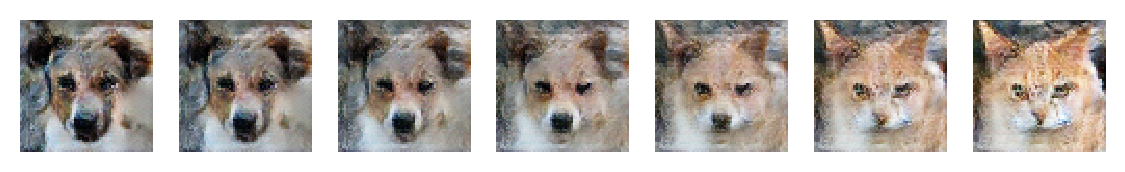
\includegraphics[width=15cm]{images/interpolation.png}
\caption{Generált képek lineáris interpolációval két zajvektor között}
\label{fig:interpolation}
\end{figure}

A bemeneti vektorok teréről feltételezhetjük, hogy folytonosan van kitöltve, mivel bármely pontra egy képet kaphatunk vissza. Viszont ezen tér feltérképezése sem egy triviális feladat, és az sem biztosított, hogy a talált pont környezetéből mintavételezve hasonló tulajdonságú képek generálhatóak ki.

A GAN tanítása során a Generátor a bemeneti vektorok terére megtanulja, hogy a tér egyes pontjaira milyen adatot képezzen le. A térből mintavételezett adatok mindegyikére egy, a tanítóhalmaz eloszlását követő adatot tud kigenerálni.
A tanítási lépések során általában normális vagy egyenletes eloszlás szerint generálunk pontokat, és azok alapján tanul a Generátor modellünk. Annak ellenére, hogy a tér egyes pontjaira igen jól betanul a modell, nem garantálható, hogy az így keletkezett tér megfelelően klaszterezhető lehet és valójában a tanítás során generált pontok eloszlását követik a klaszterek pontjai \cite{mukherjee2019clustergan}.

\Section{Képek közelítése pixel szinten}

A képek közelítésre egy megoldás lehet a \textit{synthesis-through-optimization} technika \cite{frans2021clipdraw}, amelyhez nem kell betanítani egy újabb modellt, csupán optimalizációs alapon történik meg a képek közelítése.
A technika megvalósításához szükségünk van egy olyan függvényre, amely adott bemenetre egy várt kimenetet generál, ez esetünkben a Generátor modell. Az bemenetre kapott kimenetet ezután meg kell vizsgálni, és egy célfüggvény segítségével ki kell értékelni, majd a hibaérték alapján módosítani kell a bemenetet olyan irányba, hogy a hiba csökkenjen.

A kimenet vizsgálatára általában egy osztályozót szokás alkalmazni. A következő alfejezetben ez a módszer kerül majd bemutatásra. Viszont a bemenet optimalizálási módszere egy egyszerűbb vizsgálati stratégia mellett kerül bemutatásra az egyszerűbben érthetőség kedvéért.

%TODO: A jelölések egységesítése! (nem csak erre az alfejezetre vonatkozólag!)
A GAN $G$ generátorának bemenete egy $\vec{z} \in \mathbb{R}^{z_n}$ vektor, ahol $z_n$ általában 100 szokott lenni. Vagyis a bemeneti vektor egy $z_n$ dimenziójú tér egy pontja. A 100 dimenzióban történő keresés igen nehéz lehet a hagyományos heurisztikus módszerekkel, mint például a hegymászó módszerrel. A hegymászó optimalizáló módszer során a célfüggvényt minimalizáljuk (vagy maximalizáljuk) a pont körüli tartomány mintavételezésével, majd a megfelelő szomszédos pontra való lépéssel. A bemeneti paraméter lehet a pont kiinduló pozíciója, a lépésköz és a mintavételezés sűrűsége. A megfelelő pontosság érdekében igen sok mintára lehet szükségünk, egy sokdimenziós térben pedig igen sok minta szükséges a tér feltérképezésére. A fix lépésköz és a mintavételezés pontatlanságának hatására könnyedén lokális optimumokban ragadhat az algoritmus. Több vizsgálandó pont elszórása a térben megnövelheti az esélyét annak, hogy rátalálunk a globális optimumra is, viszont ez jelentősen megnöveli a számításigényt.

A gradiens módszer vagy gradiens-süllyesztés (\textit{Gradient Descent}) egy olyan iteratív optimalizáló módszer, amely a differenciálható függvény lokális minimumának megtalására irányul. A célfüggvény elsőrendű deriváltjai igazítják el a vizsgált pontunkat a minimumhoz \cite{ruder2016overview}. A Gradiens módszer is fix lépésközökkel közelíti az optimumot, viszont ha a tér differenciálható, úgy a lépés iránya gyorsabban számolható, mint a hegymászó módszer esetében. Az optimalizálás tehát a Gradiens módszer segítségével kerül megvalósításra.

Két kép között a pixelszintű távolságot az L2 norma (vagy euklideszi norma) segítségével kaphatjuk meg, amely az
$$ \|x\|_2 = \left({\sum_{i=1}^{n}|x_i|^2}\right)^{\frac{1}{2}} $$
formában számítható.
Ezen távolságot L2- (vagy euklideszi) távolságnak is lehet nevezni. A kép egyes pixeleinek értékeit veszi csupán figyelembe. Az összehasonlításhoz a képeket ki kell nyújtani, hogy egy-egy vektort kapjunk.

Egy kiválasztott kép közelítése a bemeneti vektorok terében a következő módon történhet. Jelölje $X$ a keresendő képet, $G$ a generátort, $\vec{z} \in \mathbb{R}^{z_n}$ pedig a látens vektort.\\
A cél egy olyan $\vec{z} \in \mathbb{R}^{z_n}$ látens vektor keresése, amellyel a
$$ \sum_{i=1}^{n\times m}\sqrt{(X_i-G(\vec{z})_i)^2}$$
távolság minimalizálható.

A képeket tehát pixel szinten hasonlítjuk össze kiindulásképp.
Egyéb metrikákat is alkalmazhatunk a képek hasonlóságának mérésére, viszont az optimalizáló módszer bemutatásához ezen legegyszerűbb módszert választottam.

Legyen $l$ a lépésméret, $X \in \mathbb{R}^{n\times m \times 3}$ a keresendő kép, $G$ pedig a betanított Generátor. Jelöljük $t$-vel az időpillanatot.
\begin{enumerate}
	\item Generáljunk egy képet az aktuális $\vec{z}$ zajvektorral:
$$\hat X = G(\vec{z}).$$
	\item Számoljuk ki a generált kép és a keresendő kép távolságát:
$$ loss(\vec{z}) = \sum_{i=1}^{n\times m}\sqrt{(X_i-\hat X_i)^2}. $$
	\item Számoljuk ki a gradienseket a hibafüggvény szerint:
$$ grad(\vec{z}) = \frac{\mathrm{d}}{\mathrm{d}\vec{z}} \; loss(\vec{z}).$$
	\item Módosítsuk a $\vec{z}$ zajvektor elemeit a kapott gradiensek szerint egy $l$ hosszúságú lépéssel:
$$ \vec{z}^{\;(t)} = \vec{z}^{\;(t-1)} - l \cdot grad\left(\vec{z}^{\;(t-1)}\right).$$
	\item Ismételjük meg az algoritmust a konvergálásig.
\end{enumerate}

A kilépési feltétel nincs megadva, így az algoritmus előre meghatározott iterációszámig fut. A hibafüggvények változását esetleg nyomon követhetnénk, és ha két érték között oszcillál a hibafüggvény, akkor valószínűleg elért az algoritmus egy lokális minimumot. A példa egyszerűsítése kedvéért a lépésszám is egy bemeneti paraméter jelen esetben.

Az algoritmus Tensorflow-ban történő megvalósítása a következő:

\begin{python}
random_noise = tf.random.uniform([1, latent_dim], minval=-1, maxval=1)
noise = tf.Variable(random_noise)
step_size = 0.03
steps = 50
for i in range(steps):
    with tf.GradientTape() as g_tape:
        g_tape.watch(noise)
        generated_image = generator(noise, training=False)
        loss = tf.norm(goal_image - generated_image)
    gradients = g_tape.gradient(loss, noise)
    noise = noise - (step_size * gradients)
\end{python}

Az implementációban ügyelni kell arra, hogy a gradiensek meghatározásához szükséges változókon ne hajtsunk végre a TensorFlow-n kívüli módosításokat, hiszen olyankor a TensorFlow nem képes visszakövetni a gradiens számolást. Tehát ha például a számolás során mátrix műveleteket kell alkalmazunk a változóinkra, akkor azt egy külső csomag, például NumPy segítségével sajnos nem tehetjük meg. Viszont a TensorFlow-ban is megtalálhatóak a NumPy csomagból ismert eljárások, sokszor teljesen megegyező névvel és paraméterezéssel. Azért, hogy a bemeneti zajvektort módosítani lehessen, egy \texttt{tf.Variable} objektumot inicializálunk a zaj értékével. Ha ezt nem tennénk meg, a generált zaj konstans lenne, amelyet a módszer nem tudna megváltoztatni.

A Gradiens süllyesztés alapvető esetben fix lépésközökkel kerül végrehajtásra, viszont egy egyszerű bővítése lehet a módszernek a momentummal való kiegészítés. A momentum érték hatására a vizsgált pont nem csupán fix lépésekkel közlekedik a felületen, hanem a korábbi lépésköz figyelembe vételével változik az iterációkban elvégzett lépés távolsága.

Momentum esetén a változás a következőképpen kapható meg:
\begin{align*}
valtozas^{(t)} &= l \cdot \vec{grad} + momentum \cdot valtozas^{(t-1)}, \\
z_i^{(t)} &= z_i^{(t-1)} - valtozas^{(t)}.
\end{align*}

A momentum értékét 0 és 1 között szokás megadni. 0 momentum esetén valójában a momentum nélküli gradiens módszert kapjuk vissza.

Az alábbi kódrészletben egy olyan függvény található, amelyben a momentummal kiegészített gradiens módszer került implementálásra.
\begin{python}
def gradient_descent_momentum(goal_image, noise, step_size,
                              momentum, steps):
    change = 0
    for i in range(steps):
        with tf.GradientTape() as g_tape:
            g_tape.watch(noise)
            generated_image = generator(noise, training=False)
            loss = tf.norm(goal_image - generated_image)
        gradients = g_tape.gradient(loss, noise)
        change = (step_size * gradients) + momentum * change
        noise = noise - change
    return noise
\end{python}

A képek visszakeresésére $l=0.2$ lépésközzel és $0.9$ körüli momentum értékkel indítottam el az algoritmust. Ezen értékek megfelelőnek tűntek, viszont a paraméterek nagyban függnek a vizsgálandó Generátortól. A kép felbontásától, a látens dimenzió számától és a kiinduló zajtól is függ a paraméterek megválasztása.
A kiinduló zajt a pixelszintű visszakeresésnél az egyenletes eloszlásból generáltam ki a $[-1; 1]$ intervallumon. A bemeneti zajvektor eloszlása is egy olyan paraméter, amellyel érdemes kísérletezni.

\Aref{fig:gradlosses}. ábrán megfigyelhető a kétféle gradiens keresés során kapott hibaértékek változása, a kezdeti és a kiinduló zajvektor a keresés előtt és után, továbbá az ábra alján az egyes időpillanatokban kigenerált képek. Az ábrán megfigyelhető, hogy a momentum nélküli keresés során a konvergencia görbe sokkal simább, viszont hamar elér egy optimum pontot, amelyben megragad és nem képes ezután olyan nagy mértékben csökkenteni a hiba értéket. Ezzel szemben a momentummal történő keresés szemmel láthatóan átlépett ezen az optimumon a lendülete segítségével amikor a hibaértékei növekvő értékeket mutattak, majd egy olyan utat járt be, amely során jobban közelítette a keresendő zajvektort.

\begin{figure}[h]
\centering
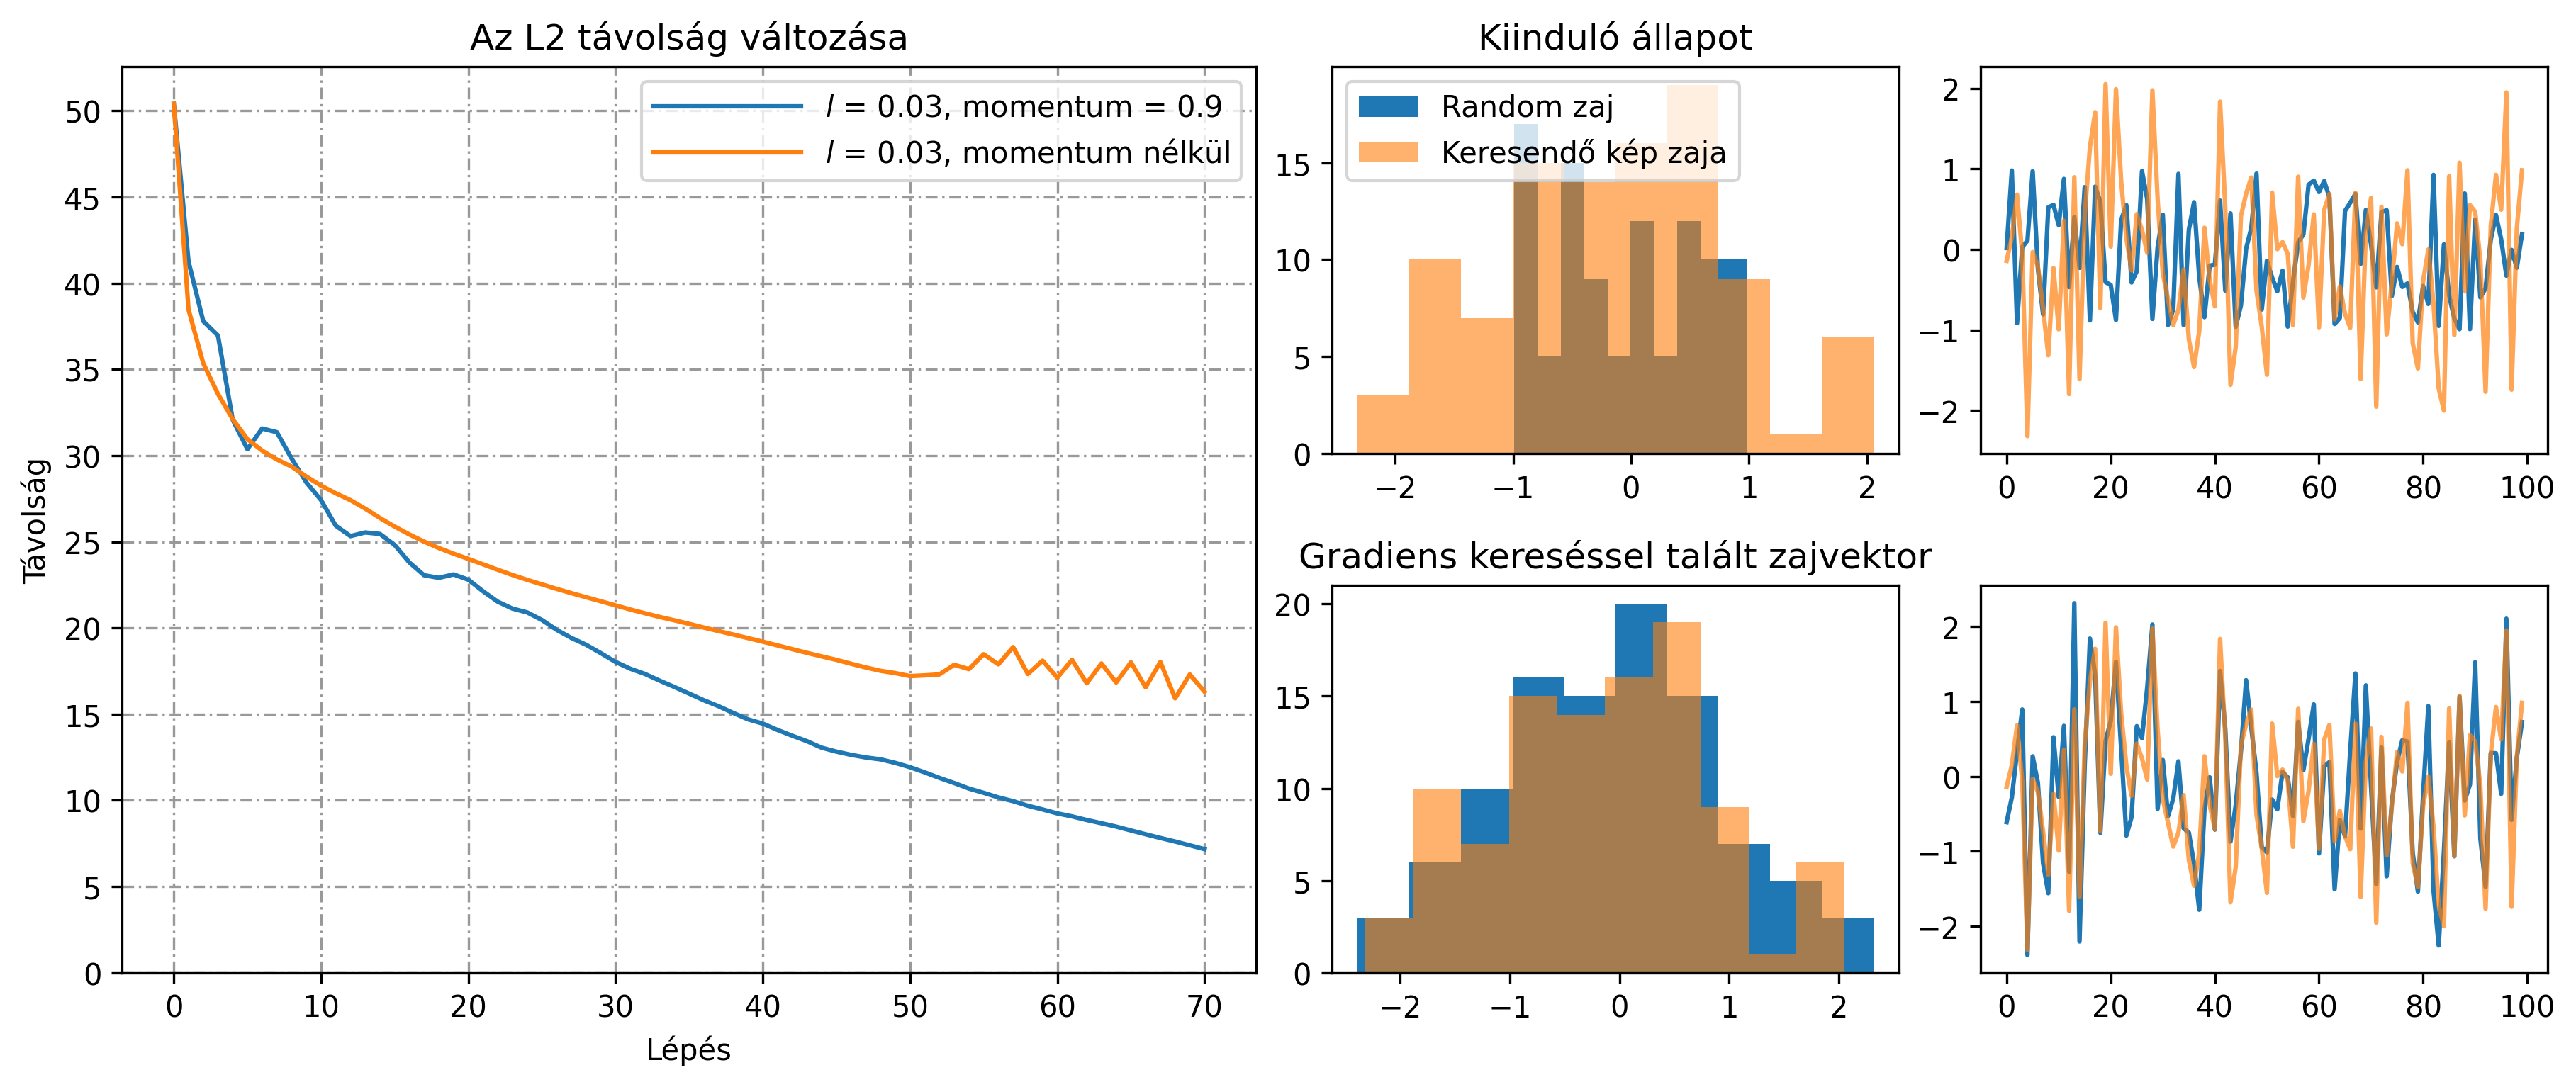
\includegraphics[width=15cm]{images/grad_losses.png}
\caption{A hibafüggvény változása a lépések során}
\label{fig:gradlosses}
\end{figure}

\Aref{fig:gradfound}. ábrán a keresendő zajvektorból generált kép, a kiinduló zaj képe és a momentum nélküli és a momentummal talált kimenet figyelhető meg. A momentummal történő keresés pontosabb találatot eredményezett, a momentum nélkül pedig igen közeli lokális optimum pontot kaptunk.

\begin{figure}[h]
\centering
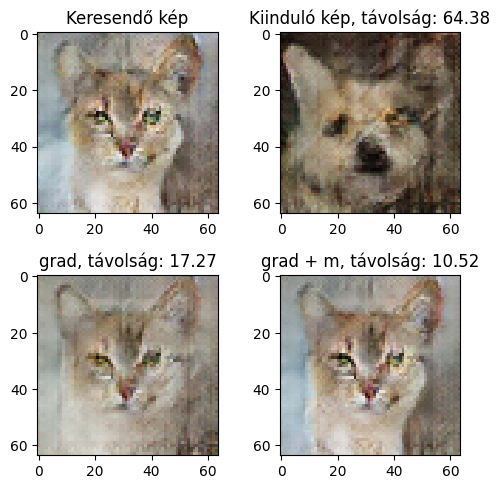
\includegraphics[width=8cm]{images/grad_found.png}
\caption{Gradiens kereséssel visszakeresett képek}
\label{fig:gradfound}
\end{figure}

\Aref{fig:gradval}. ábrán pedig egy, az adathalmaz validációs részéből kiválasztott képének visszakeresésének eredményét figyelhetjük meg. Ezen képet a GAN modell nem látta a tanulás során, viszont a kapott eredmény szemmel láthatóan egy corgi-t ábrázol, még ha nem is olyan kidolgozottan.

\begin{figure}[h]
	\centering
	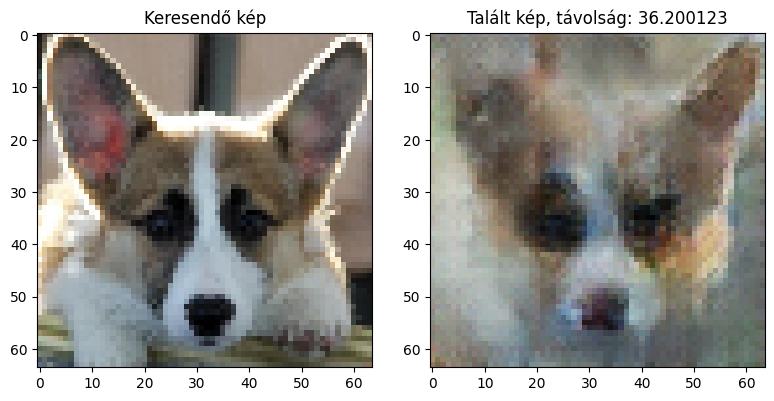
\includegraphics[width=8cm]{images/grad_search_val_image.png}
	\caption{A validációs halmaz egyik elemének visszakeresése}
	\label{fig:gradval}
\end{figure}


\Section{Képek keresése osztályozó segítségével}

A képek visszakeresése pixel szinten csupán azokban az esetekben adhat igazán jó megoldást, amikor a Generátor egy korábbi kimenetére végezzük el a keresést. Az előbbiekben erre láthattunk példát, \aref{fig:gradfound}. ábrán is az figyelhető meg, hogy a korábban kigenerált kép bemeneti vektorát hogyan sikerült a gradienslejtési módszerekkel (momentum nélkül és momentummal) visszakeresni.
Viszont ha egy külső forrásból érkező képet kívánunk így visszakeresni, akkor az eredményül kapott vektorból generált kép nem fogja olyan jól közelíteni a keresendő képet, hiába sikerült minimalizálnia a távolságot.
Ez értelemszerűen abból adódik, hogy az algoritmus a keresés során a nyers pixelértékeket veszi csupán csak figyelembe, a kép tartalmára tehát semmiféle információja nincsen. Viszont a Generátor nem képes minden pixelét egymástól függetlenül változtatni, hiszen a dekonvolúciós rétegeknek köszönhetően betanulta a tanítóhalmaz jellegzetességeit, és a kigenerált képek is a tanítóhalmaz eloszlását követik. Így nem létezhet olyan bemeneti vektor, amellyel tetszőleges pixelértékeket felvehet a kimeneti kép.

Ha az eredeti adathalmazból  kívánunk képeket visszakeresni, akkor közelítő eredményeket kaphatunk (mint ahogyan az \aref{fig:gradval}. ábrán is látszik), viszont ezek továbbra sem lesznek tökéletes találtatok, hiszen a GAN nem pixel pontosan tanulja be az adathalmaz elemeit, hanem azok jellegzetességeit tanulja meg reprezentálni, ezért is nevezik a GAN-t \textit{Representation-learning} \cite{geron2019hands} modellnek is.

Ha a hibafüggvényt kicseréljük, és az optimalizációt egy, az adathalmazon tanított osztályozóval végezzük el, úgy viszonylag jó találatot kaphatunk. Természetesen ilyenkor az osztályozó teljesítményétől is függ az eredmény jósága.

Az irodalomkutatás során egyetlen munkát találtam, amely publikálva is volt (CLIP\-DRAW \cite{frans2021clipdraw}), amely ilyen megoldást használ. A további ismertebb munkák csupán notebook-ok formájában érhetőek el. Viszont a közös bennük, hogy mind a CLIP \cite{radford2021learning} osztályozó kimenetei alapján végzik el az optimalizációt.

Egy hasonló megoldást alkalmaztam, viszont a CLIP osztályozó helyett egy saját modellt tanítottam be. A betanított osztályozó modell alapja az Inception v3, amely a témám során több helyen is feltűnt, az IS és FID pontok számítása is ezen modellen alapszik. Az ImageNet \cite{deng2009imagenet} adatbázison tanított Inception modell az adatbázis 1000 darab osztályára képes osztályozni. Ha a modellt használni kívánjuk a saját osztályozónkba, akkor az úgynevezett \textit{Transfer-learning} \cite{tensorflow} technikát kell alkalmazni a tanításhoz, amelynek lényege, hogy egy, már betanított általános modellre egy újabb modellt építünk, amely egy szűkebb, speciális feladat megoldására szánunk. Esetünkben nincs szükség 1000 darab osztályra. Az Inception modellt felhasználhatjuk a képek jellegeinek kinyerésére, és a modell utolsó rétegét pedig kicseréljük a saját osztályozónkra. A kapott modell tanítása egyszerűbbé válik, mintha az alapoktól kellene egy új modellt betanítanunk.

A tanítás során az eredeti modell súlyait "lefagyasztjuk", vagyis a háló ezen részének paramétereit taníthatatlanná tesszük, és a tanítás során csak az általunk hozzáadott rétegeket frissítjük.
A hibafüggvény számoláshoz a Kategórikus Kereszt-entrópiát (\textit{Categorical Cross-Entropy}) használjuk fel. Az osztályozó modell tanítása ezek után a teljesen megszokott módon történik.

Az alábbi kódrészletben az osztályozó modell implementációja figyelhető meg.
\begin{python}
inputs = keras.Input(shape=(64, 64, 3))
x = data_augmentation(inputs)
resized = tf.image.resize(
    x, [299, 299],
    preserve_aspect_ratio=True, method='nearest'
)
x = inception_model(resized, training=False)
x = keras.layers.GlobalAveragePooling2D()(x)
x = keras.layers.Dropout(0.2)(x)
x = keras.layers.Dense(3)(x)
outputs = keras.layers.Activation("softmax")(x)
model = keras.Model(inputs, outputs)
\end{python}

Az újonnan kialakított modell bemenete megegyezik a betanított Generátor kimenetével. Az \textit{overfitting} elkerülése érdekében, és hogy a modell ne az egyes, számára érdekes pixelértékek alapján hozza meg a döntést, a bemenetre \textit{data augmentation} technika kerül alkalmazásra, amely véletlenszerű minimális transzformációkat alkalmaz a képekre. A bemeneti képeket véletlenszerűen függőlegesen tükrözi, és szintén véletlenszerűen elforgatja. A Cifar-10 adathalmaz esetében azt figyeltem meg, hogy az augmentation technika csak megnehezíti a konvergenciát, és a modell nagyon sokat tévedett ennek hatására. A technika kihagyásával a tanítás jobb eredményt hozott, viszont ezen adathalmaz sokkal több tanítómintával rendelkezik, mint az AFHQ és a benne található képek is változatosabbak, így esetében lehetséges, hogy valóban nem indokolt a technika használata.

Az \texttt{inception\_model} a kódrészletben a már említett, csonkított változata az eredetinek. Az utolsó \texttt{Dense} rétegétől megfosztott változata, a lefagyasztott súlyokkal. Az Inception modell bemenetként $299 \times 299$ felbontású képet vár, így a képünket fel kell nagyítani a kívánt felbontásra. A nagyításhoz \textit{nearest} interpolációt alkalmaztam, hogy a felbontás növelése ne járjon homályossággal, ugyanis azt figyeltem meg, hogy olyankor a modell gyengébben teljesít.

A csonkított Inception modell kimenete egy $(8, 8, 2048)$ alakú tenzor, amely a bemeneti képekből kinyert feature-öket tartalmazza. A \texttt{GlobalAveragePooling2D} réteg az előbbi kimenetből 2048 elemű vektort készít, amelyet beadhatunk az utolsó \texttt{Dense} rétegnek, amely az osztályozást végzi el. Egy regularizációs technikaként, hogy csökkentsük az overfitting esélyét, egy \texttt{Dropout} réteg is helyet kapott a teljesen összekapcsolt réteg előtt.
A kimenetet \texttt{softmax} aktivációs függvénnyel normalizáljuk, így a modell használata során kimenetként megkapjuk az egyes osztályokhoz tartozó valószínűségi értékeket.

A kapott modellnek összesen 21 808 931 darab paramétere van, melyből csupán 6147 a tanítható. A tanítás során tehát az osztályozásért felelős rétegeket kell csupán frissítenünk.

Az optimalizálást a GAN tanításánál is használt Adam optimalizálóval végeztem, 0.0001 \textit{learning-rate} paraméterrel. A bemeneti dataset-et 32 elemű mini-batch-ekre osztottam fel. A tanítást mindösszesen 10 epoch-ig futtattam. A nagy tanítóminta és a kevés tanítható paraméter miatt azt figyeltem meg, hogy elegendő ennyi tanítás is. A konvergenciagörbe a Cifar-10 dataset-re tanítva \aref{fig:transfer_learning_loss}. ábrán látható, az osztályozás eredményeit bemutató confusion mátrix pedig \aref{fig:transfer_confusion}. ábrán.

\begin{figure}[h]
	\centering
	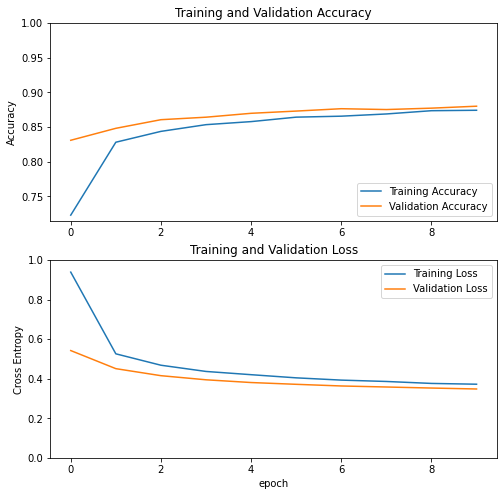
\includegraphics[width=10cm]{images/transfer_inception.png}
	\caption{Transfer-learning loss értékek (Inception modell alapú)}
	\label{fig:transfer_learning_loss}
\end{figure}

\begin{figure}[h]
	\centering
	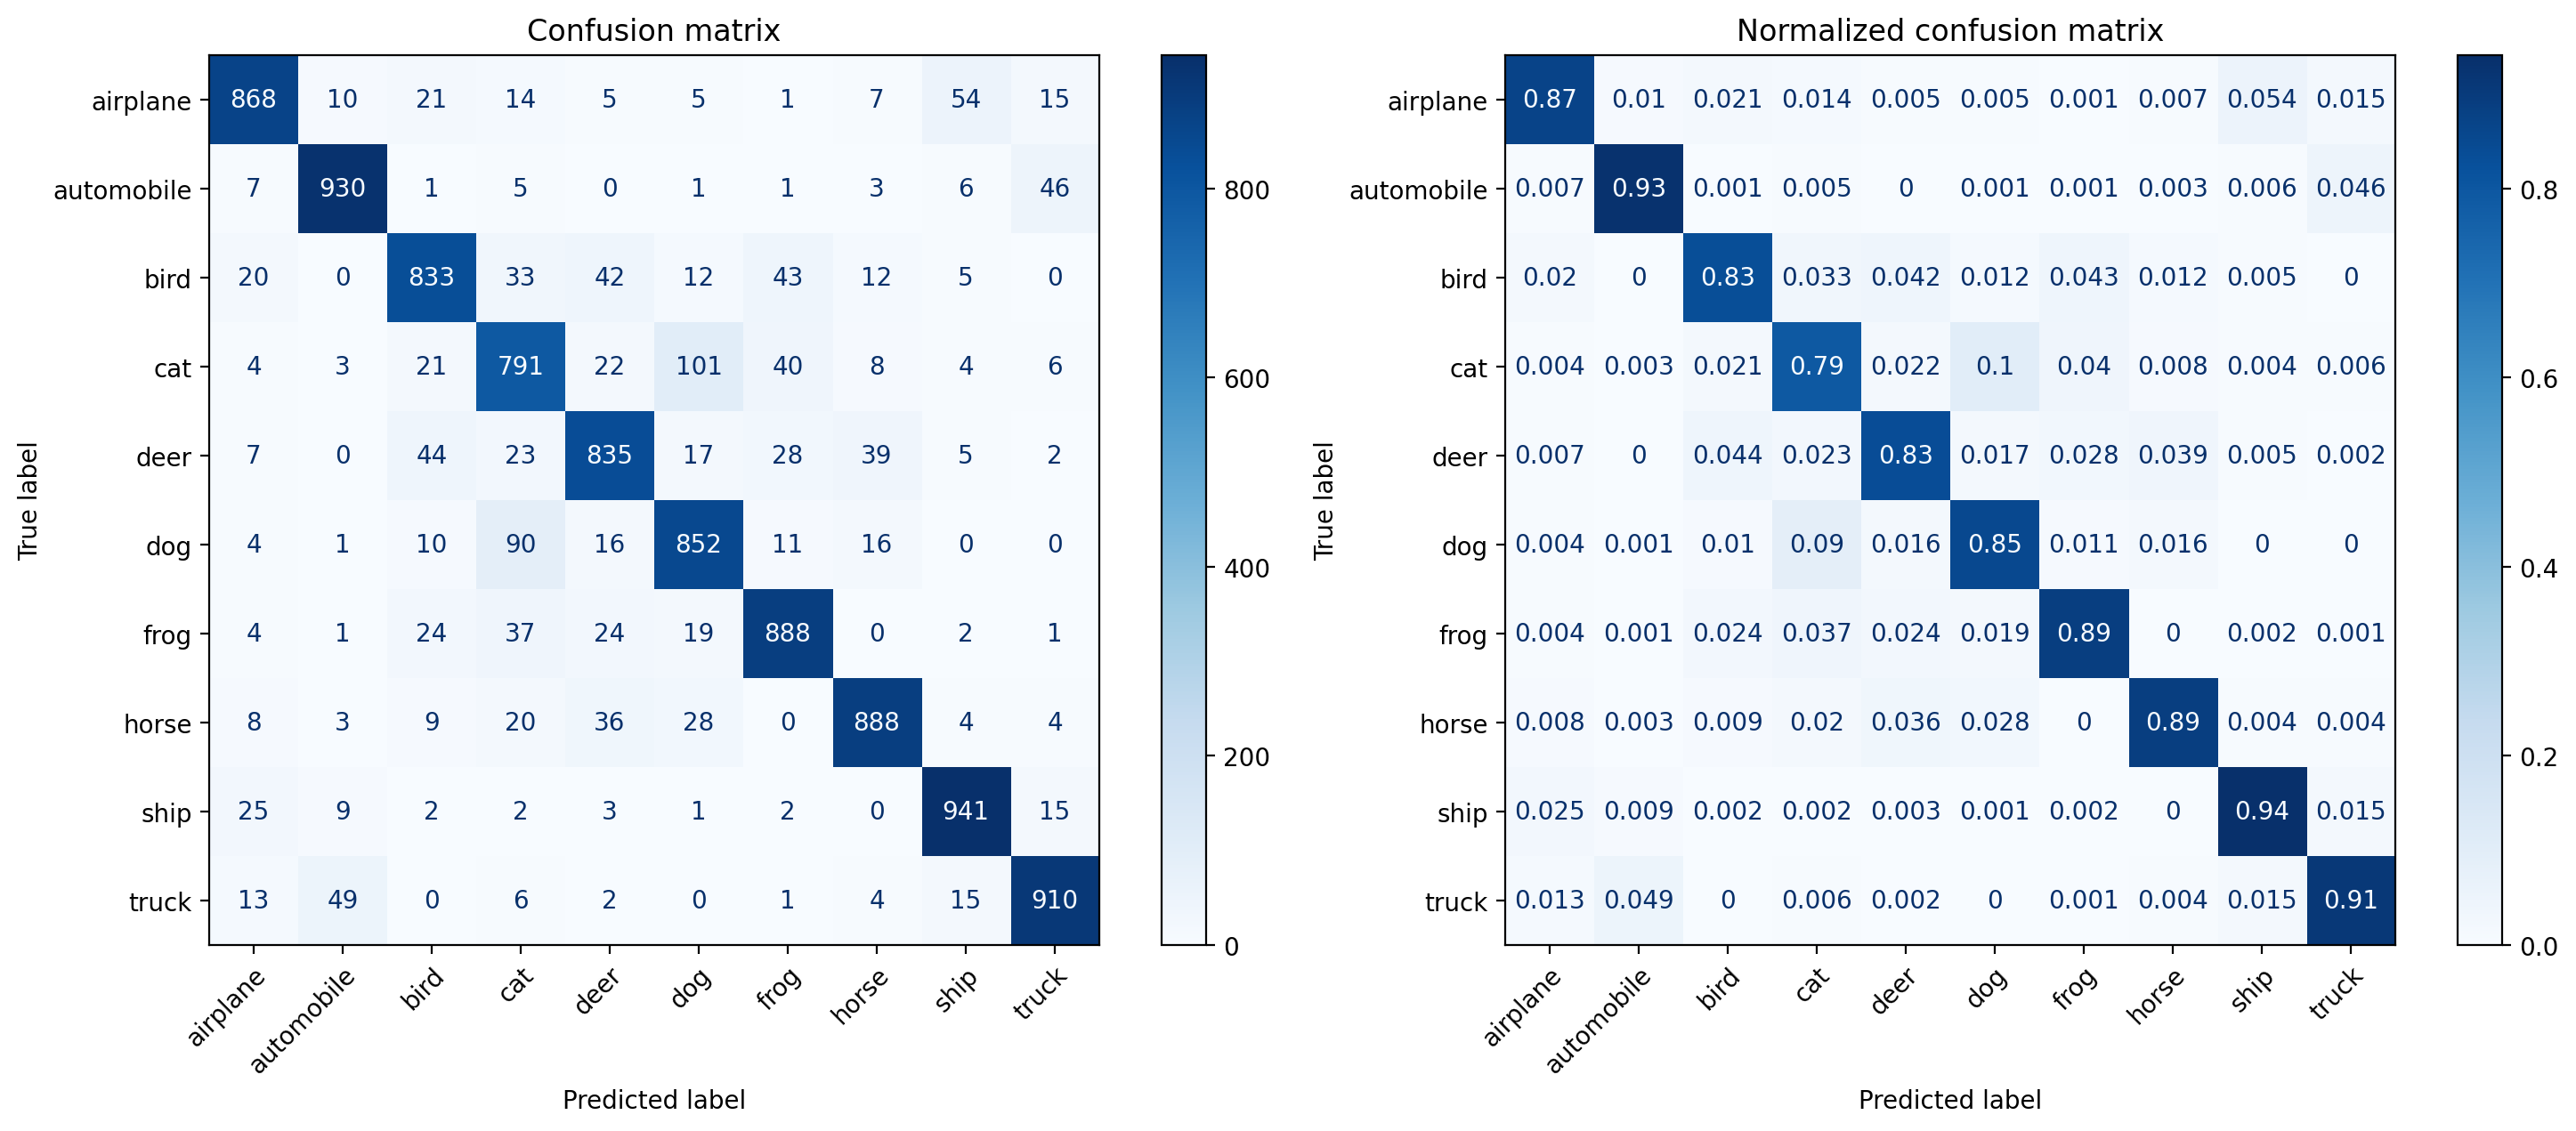
\includegraphics[width=15cm]{images/transfer_confusion.png}
	\caption{Confusion mátrix (Inception modell alapú)}
	\label{fig:transfer_confusion}
\end{figure}

Mivel a GAN tanítása után a Diszkriminátort elhagyjuk, és további szerepe nincsen, úgy gondoltam, hogy akár hasonló módon is felhasználásra kerülhet, mint az előbbiekben ismertetett Inception modell. A tanulás során természetesen nem csupán a tanítóhalmazt látta a Diszkriminátor, hanem a generált képeket is, így elég specifikus tudással rendelkezik csupán. A háló súlyai úgy lettek optimalizálva, hogy belső reprezentációt állítson elő, amellyel a bináris osztályozást megfelelően el tudja végezni. Így a háló által kinyert jellegvektorok is oly módon állnak össze, hogy el tudja az alapján dönteni, hogy a kép valódi vagy hamis. A tanítást elvégeztem, viszont az így kapott összeállított új modell teljesítménye alulmaradt az Inception-t használó másik modellel szemben. A konvergencia görbe \aref{fig:transfer_learning_loss_discriminator}. ábrán figyelhető meg, a confusion mátrix pedig \aref{fig:transfer_confusion_disc}. ábrán látható.

\begin{figure}[h!]
	\centering
	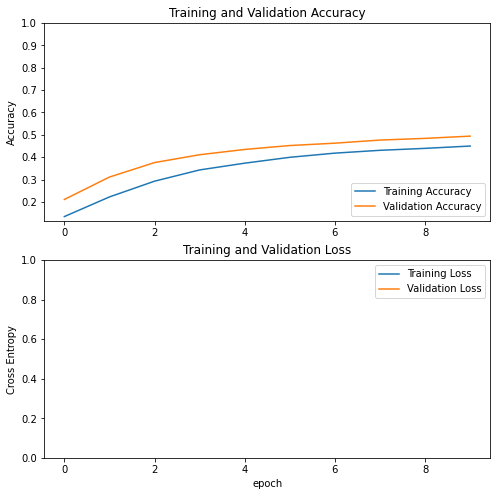
\includegraphics[width=10cm]{images/transfer_discriminator.png}
	\caption{Transfer-learning loss ábra (Diszkriminátor modell alapú)}
	\label{fig:transfer_learning_loss_discriminator}
\end{figure}

\begin{figure}[h!]
	\centering
	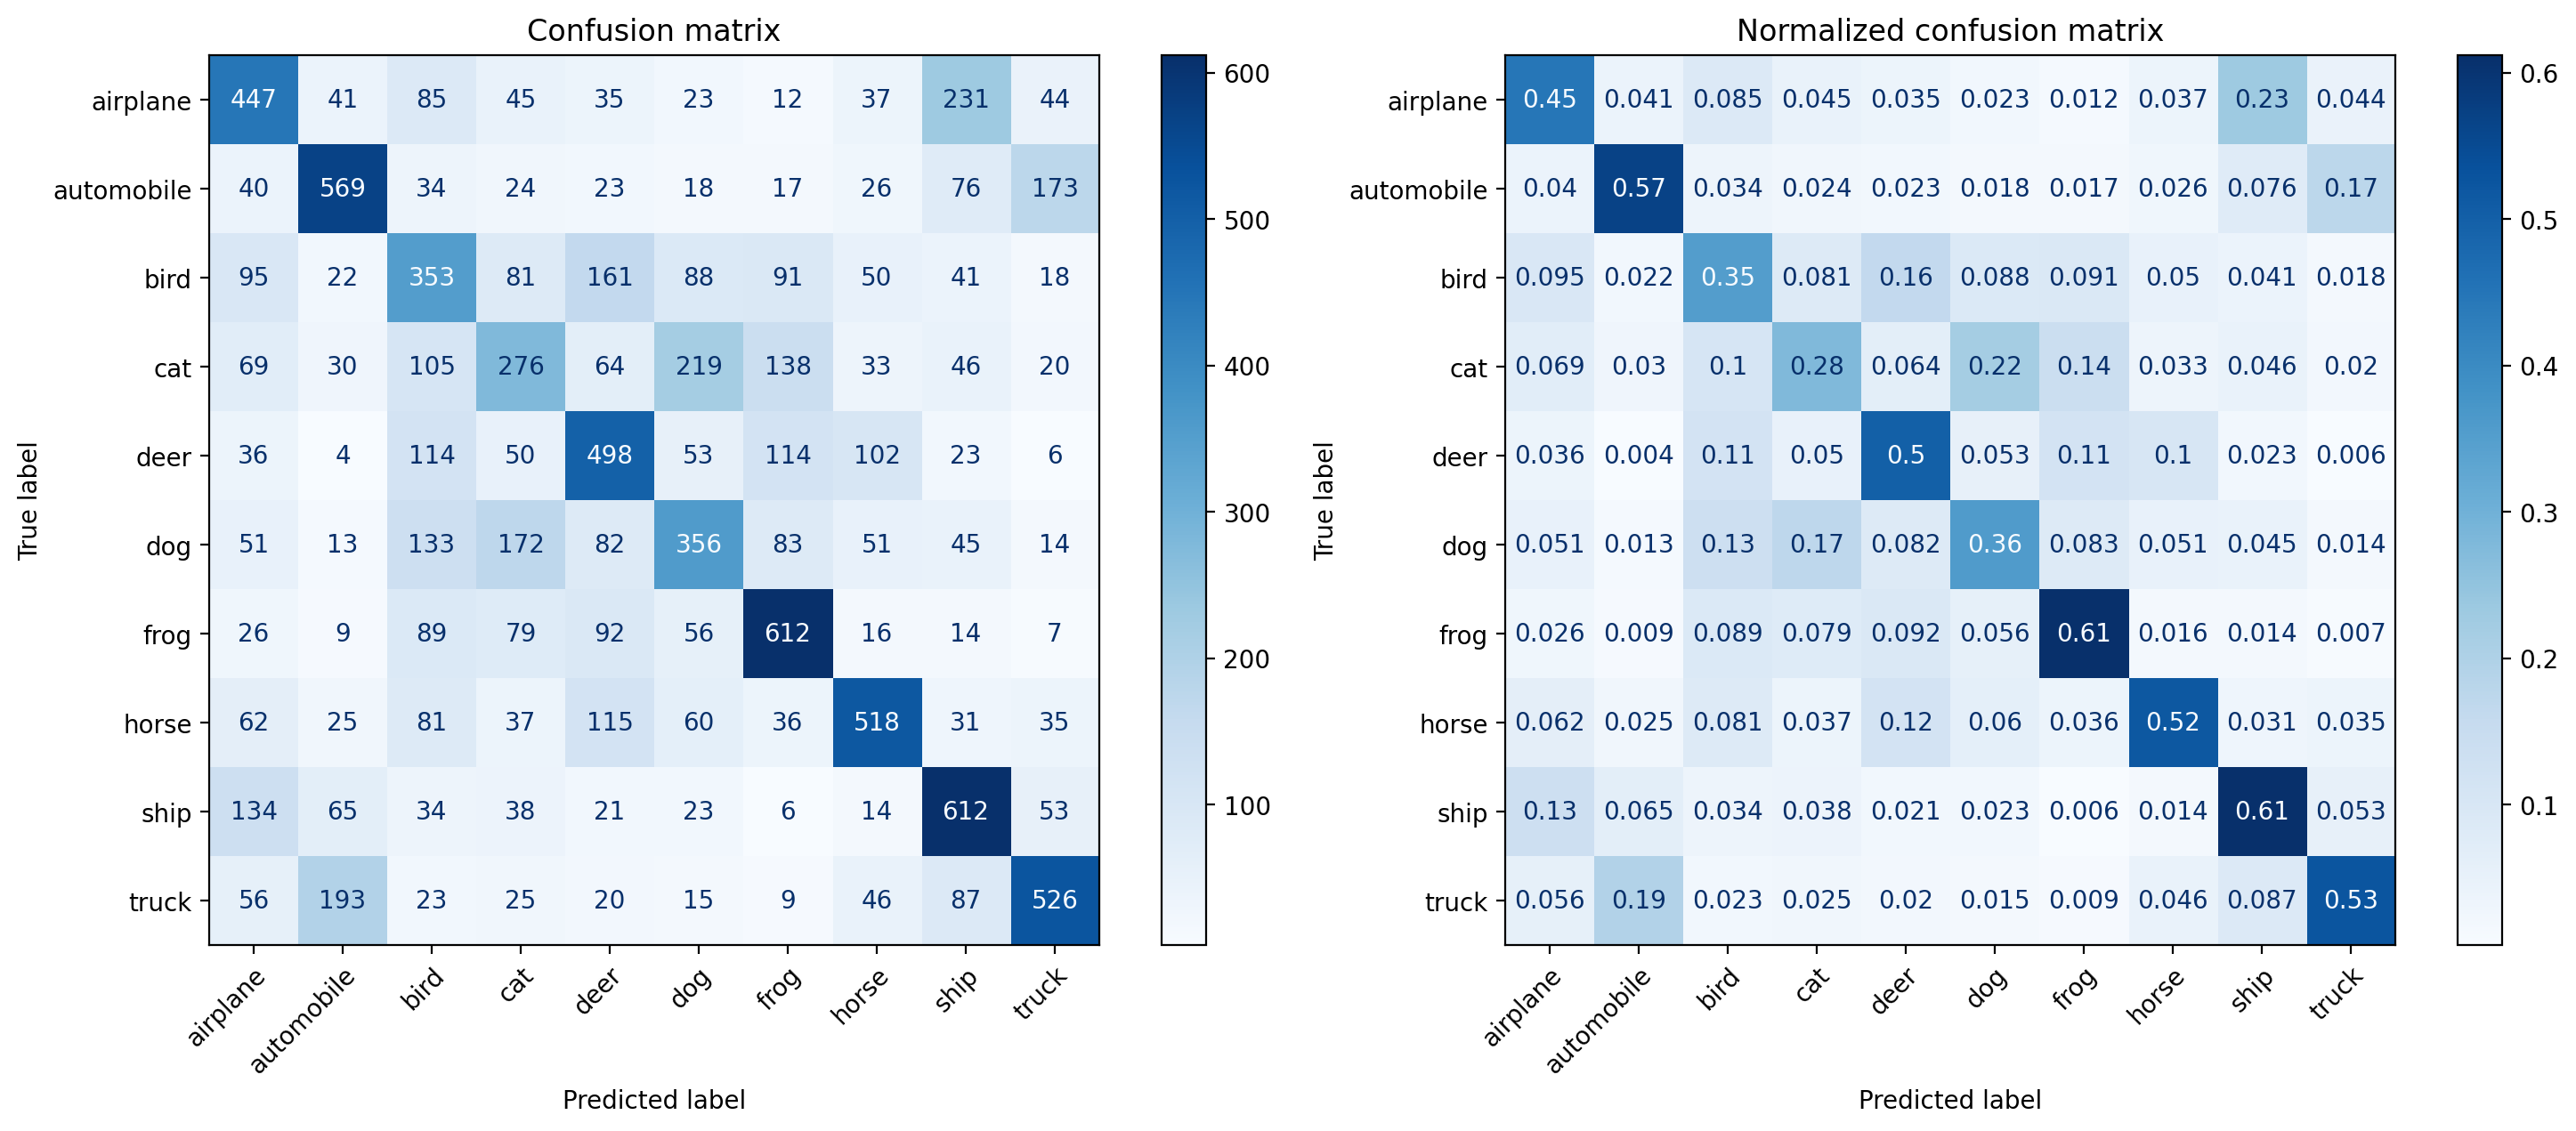
\includegraphics[width=15cm]{images/transfer_discriminator_confusion.png}
	\caption{Confusion mátrix (Diszkriminátor modell alapú)}
	\label{fig:transfer_confusion_disc}
\end{figure}


A bemeneti vektorok visszakeresése pedig a már ismertetett gradiens süllyesztés módszerrel valósul meg, viszont a hibafüggvény számolása a Kategórikus Kereszt-entrópia által kerül meghatározásra, hasonlóan, mint az osztályozó tanításánál. Az algoritmus bemenete tehát a kezdeti zajvektor, a keresendő címke és a gradiens módszer paraméterei (a lépésköz, a momentum és az iterációszám).
A bemeneti címkét \textit{One-Hot} enkódolással kell megadni a keresztentrópia számoláshoz, ugyanis az új osztályozó modell kimenete az adott osztályok valószínűségi értékei lesznek. A gradiens kereséssel pedig a keresztentrópia értéket kívánjuk csökkenteni. Tehát ha egy adott osztályra kívánunk egy olyan vektort kapni, amelyből a megfelelő osztályba tartozó képet ki tudja generálni a Generátor, akkor ebben az esetben az osztályhoz tartozó valószínűségi érték 1 lesz, a többi osztályé pedig 0.

Amennyiben kevert osztályra kívánunk képet generálni, úgy olyan keresendő one-hot enkódolást kell megadnunk, amelyben a kívánt osztályok megfelelő súlyokkal rendelkeznek. Mivel a GAN tere folytonosan van kitöltve, így feltehető, hogy létezik olyan pont a térben, amely egyszerre több osztály jellegzetességeit is magában hordozza. A \ref{fig:interpolation} ábrán is megfigyelhető, hogy az interpoláció mintavételezett pontjaiban a két végpont között milyen folytonos az átmenet és a köztes állapotokban mindkét pont tulajdonságai megjelennek.

Az eljárás optimális paraméterei ebben az esetben is több tényezőtől függnek. Az osztályozó modell teljesítménye, az osztályok száma is igen nagy befolyásoló tényező lehet a megfelelő lépésköz és momentum kiválasztására.  Megfigyeléseim szerint a megfelelő eredmények elérése érdekében a lépésközt a pixelszintű kereséstől is alacsonyabbra érdemes választani, például $l=0.005$ lépésközzel és $0.09$-es momentum értékkel az AFHQ adathalmazon tanult modellekkel értékelhető találatokat kaphatunk. A túl magas lépésköz hatására a keresés során a látens tér olyan területeire is tévedhet az algoritmus, amelyre a generátor szaturált képeket tud előállítani csupán.

\Aref{fig:searching}. és \aref{fig:searching_ship}. ábrákon láthatunk példát a macska, illetve hajó címkével történő keresésre.

A \ref{fig:collapsed_mode} ábrán is szemléltetett, a generátorban kialakuló összeomlott-mode-ok a keresési folyamat során is bosszúságot okozhatnak. Amint belépünk egy ilyen területre a keresés során, az algoritmus nem képes kilépni, hiszen az osztályozó egyszerre látja mindegyik osztály jellegzetességeit a vizsgált képen.

%TODO: Input jelzése valahogy az ábrákon.

\begin{figure}[h]
	\centering
	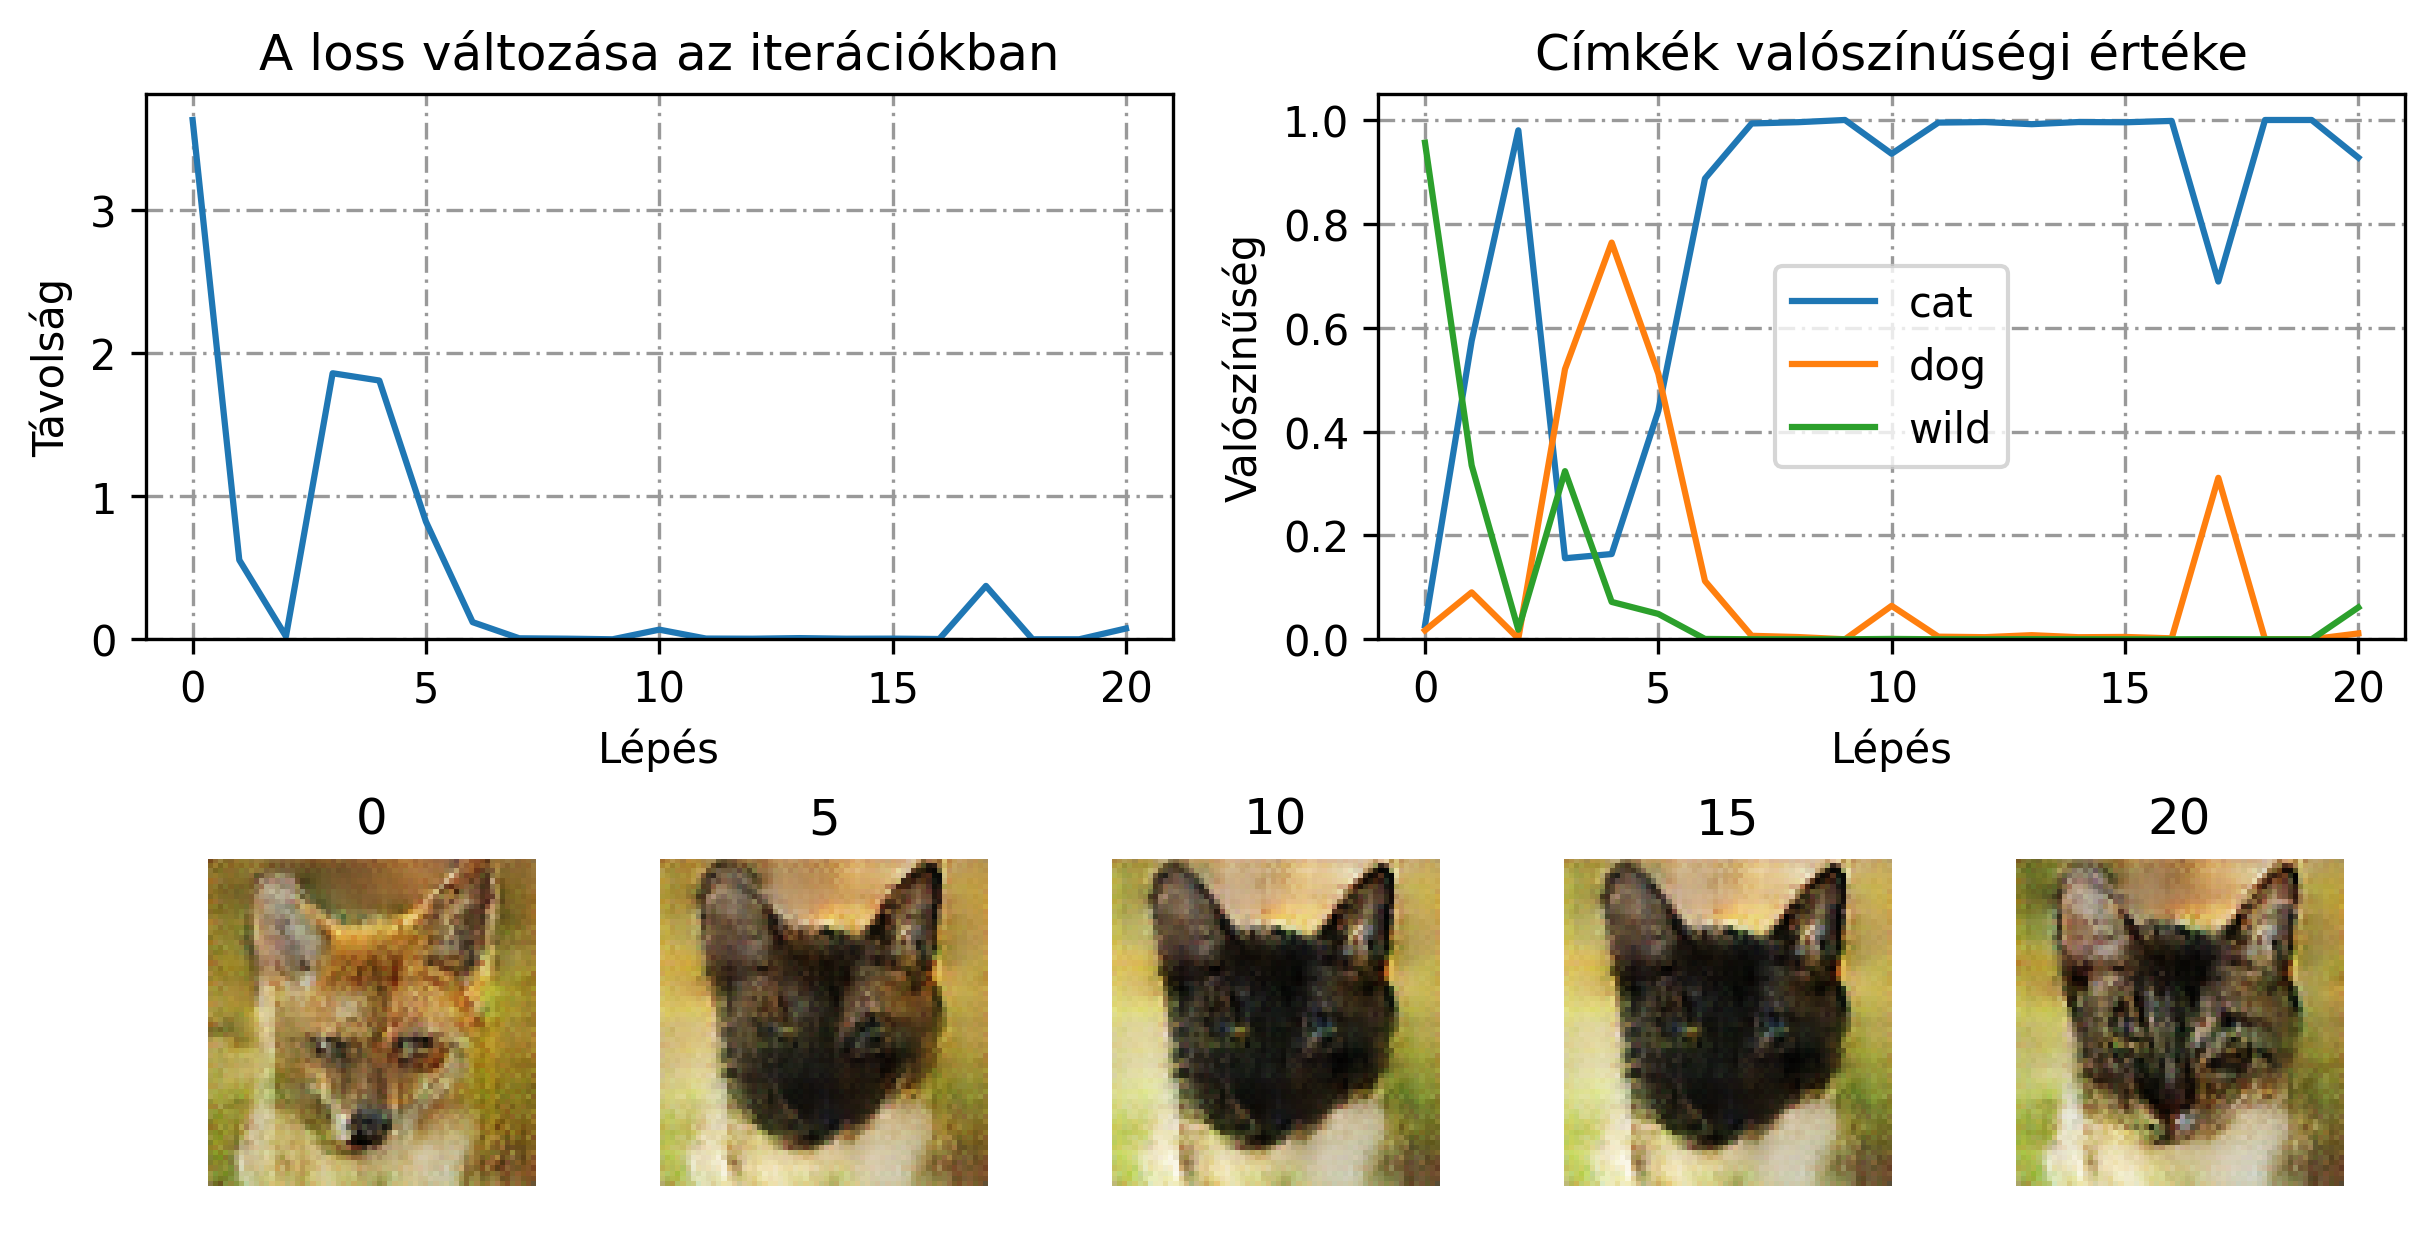
\includegraphics[width=\textwidth]{images/searching-cat.png}
	\caption{Kép generálása osztály szerint (Macska címkével)}
	\label{fig:searching}
\end{figure}

\begin{figure}[h]
	\centering
	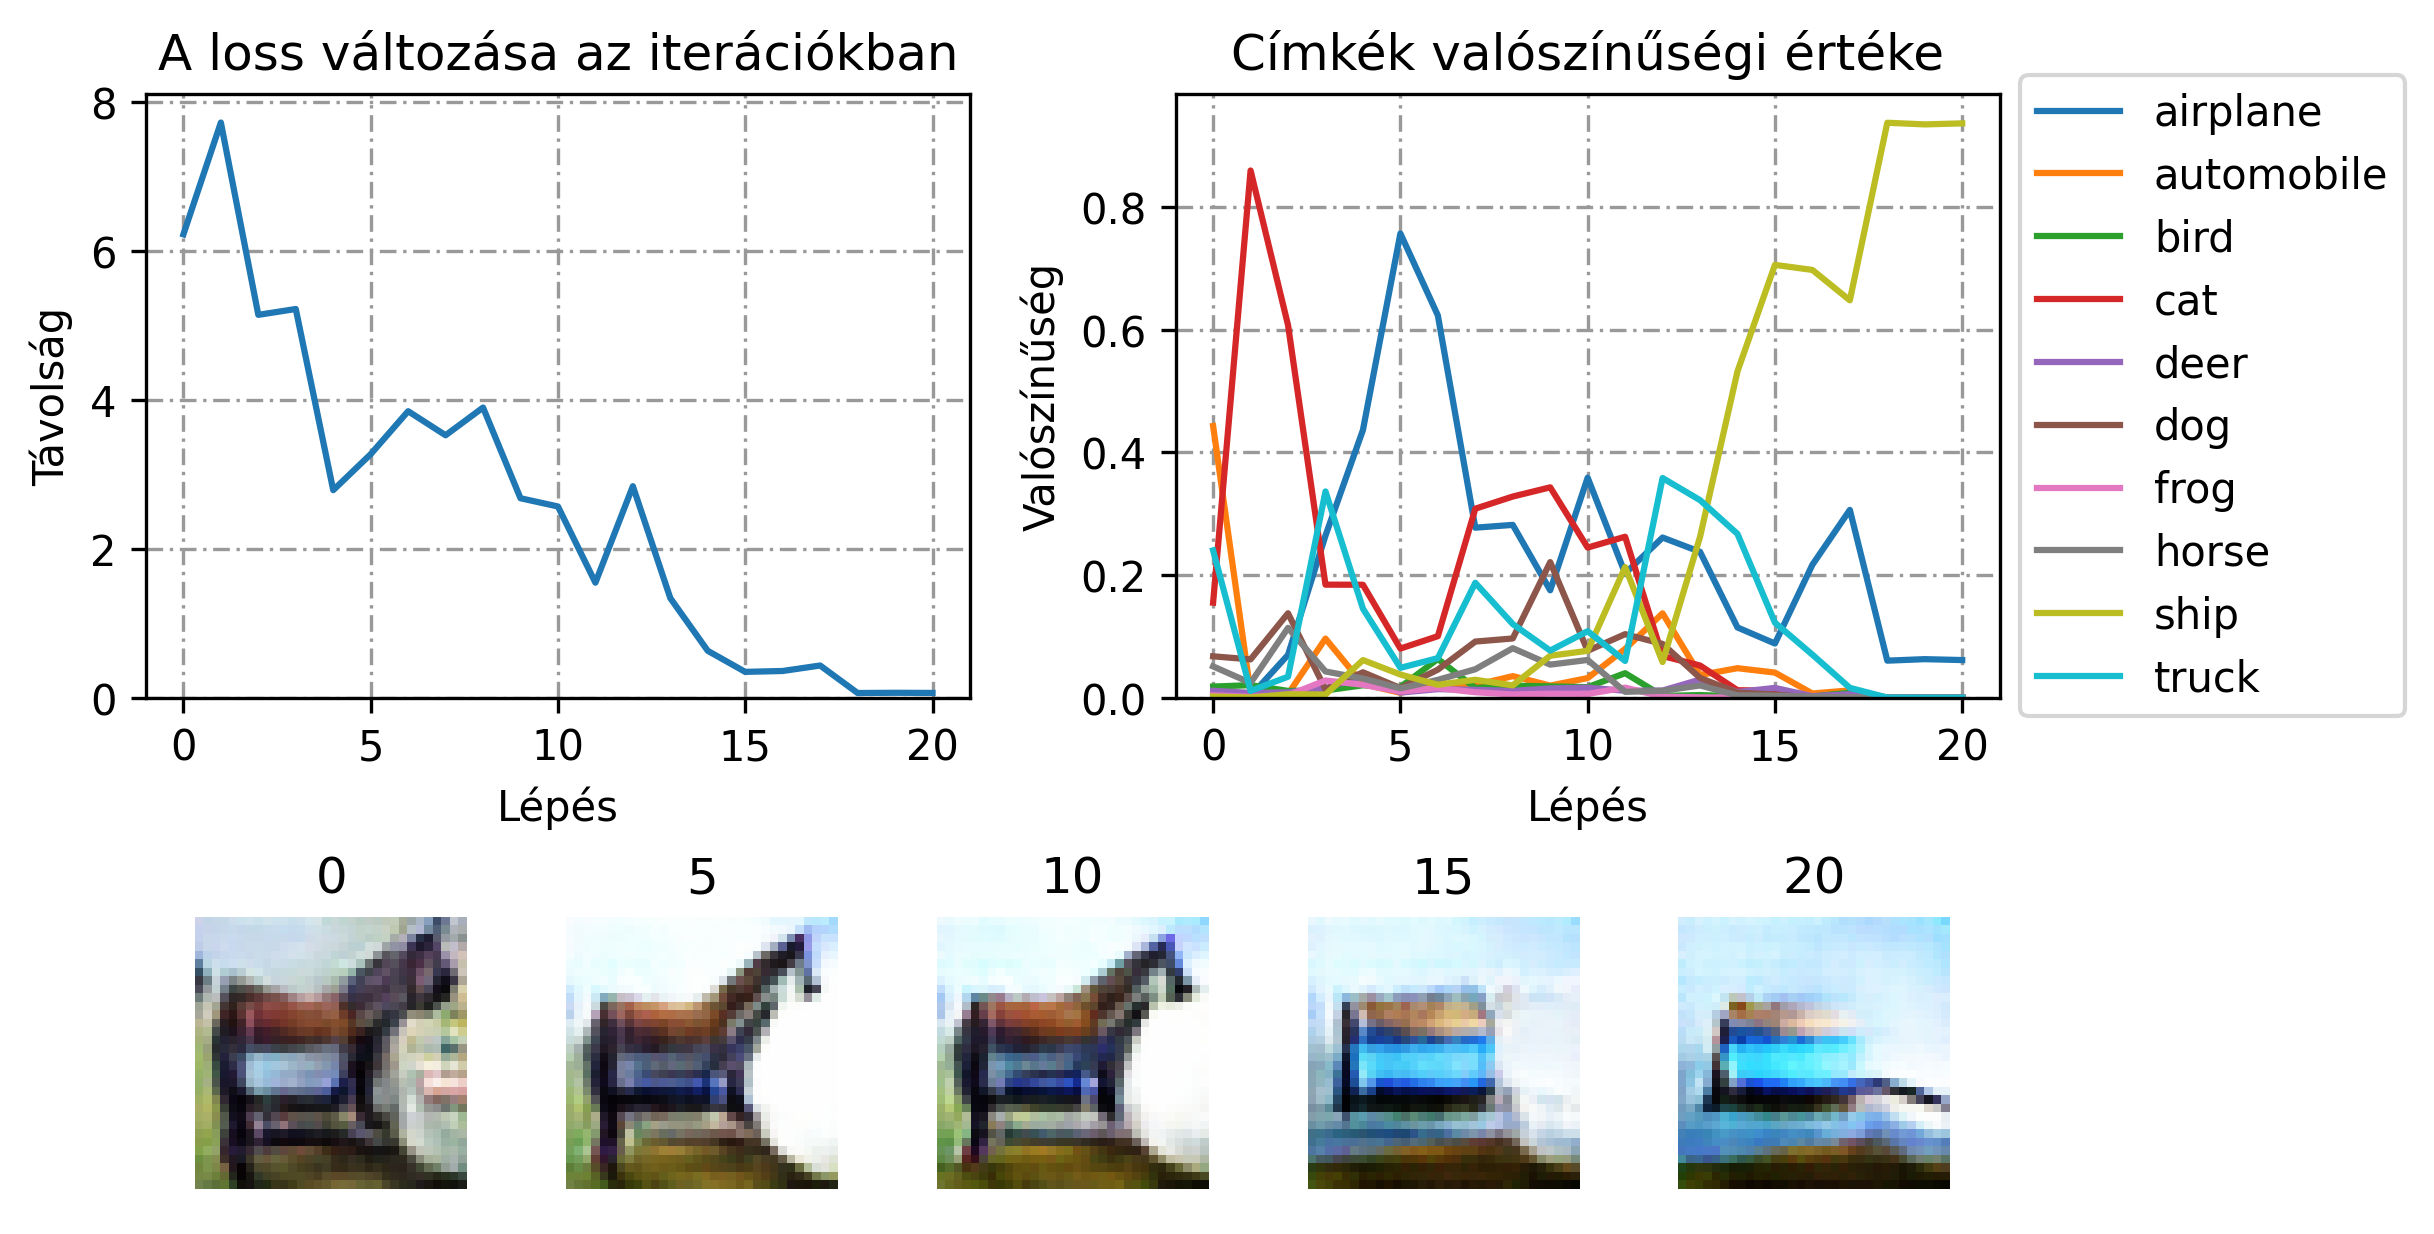
\includegraphics[width=\textwidth]{images/searching-cifar_ship.png}
	\caption{Kép generálása osztály szerint (Hajó címkével)}
	\label{fig:searching_ship}
\end{figure}



\Chapter{Demo}

%TODO Demozás! Milyen bemenetre milyen kimenetet ad? Következtetések levonása, az összeállított csomag bemutatása
\begin{figure}[h]
	\centering
	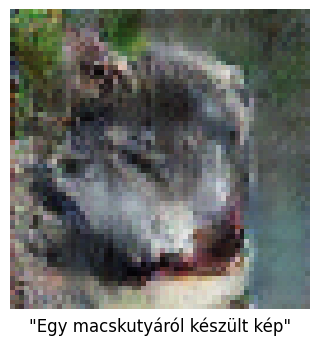
\includegraphics[width=6cm]{images/demo1.png}
	\caption{Demo kép}
	\label{fig:demo}
\end{figure}

A fejezetben be kell mutatni, hogy az elkészült alkalmazás hogyan használható.
(Az, hogy hogyan kell, hogy működjön, és hogy hogy lett elkészítve, az előző fejezetekben már megtörtént.)

Jellemzően az alábbi dolgok kerülhetnek ide.
\begin{itemize}
	\item Tesztfuttatások. Le lehet írni a futási időket, memória és tárigényt.
	\item Felhasználói kézikönyv jellegű leírás. Kifejezetten a végfelhasználó szempontjából lehet azt bemutatni, hogy mit hogy lehet majd használni.
	\item Kutatás kapcsán ide főként táblázatok, görbék és egyéb részletes összesítések kerülhetnek.
\end{itemize}
\Chapter{Összegzés}

Hasonló szerepe van, mint a bevezetésnek.
Itt már múltidőben lehet beszélni.
A szerző saját meglátása szerint kell összegezni és értékelni a dolgozat fontosabb eredményeit.
Meg lehet benne említeni, hogy mi az ami jobban, mi az ami kevésbé jobban sikerült a tervezettnél.
El lehet benne mondani, hogy milyen további tervek, fejlesztési lehetőségek vannak még a témával kapcsolatban.

\Chapter{Summary}

The content of the previous chapter in english.

\clearpage

\addcontentsline{toc}{chapter}{Irodalomjegyzék}
\bibliographystyle{unsrt}
\bibliography{dolgozat.bib}

\noindent \textit{Az internetes források utolsó ellenőrzése: 2022.04.29.}

\pagestyle{empty}

\newpage

\pagestyle{empty}

\noindent \textbf{\Large CD melléklet tartalma}

\vskip 1cm

\noindent A dolgozathoz mellékelt lemezen egy \texttt{Dolgozat} nevű jegyzékben a következő fájlok találhatóak.

\begin{itemize}
\item A dolgozat \LaTeX\ forráskódja.
\item A dolgozat PDF formátumban (\texttt{dolgozat.pdf}).
\item A magyar és angol nyelvű összefoglaló \LaTeX\ és PDF formátumban \\ (\texttt{osszegzes.tex}, \texttt{osszegzes.pdf}, \texttt{summary.tex}, \texttt{summary.pdf}).
\end{itemize}

A \texttt{Program} nevű jegyzékben található a dolgozathoz elkészített program forráskódja és futtatható változata.

\begin{itemize}
\item \textit{Feladattól, technológiától függően ez változhat.}
\item \textit{Konkretizálni kell, hogy pontosan mit tartalmaz a jegyzék!}
\end{itemize}


\end{document}
